\documentclass[polish,]{book}
\usepackage[]{mathpazo}
\usepackage{amssymb,amsmath}
\usepackage{ifxetex,ifluatex}
\usepackage{fixltx2e} % provides \textsubscript
\ifnum 0\ifxetex 1\fi\ifluatex 1\fi=0 % if pdftex
  \usepackage[T1]{fontenc}
  \usepackage[utf8]{inputenc}
\else % if luatex or xelatex
  \ifxetex
    \usepackage{mathspec}
  \else
    \usepackage{fontspec}
  \fi
  \defaultfontfeatures{Ligatures=TeX,Scale=MatchLowercase}
\fi
% use upquote if available, for straight quotes in verbatim environments
\IfFileExists{upquote.sty}{\usepackage{upquote}}{}
% use microtype if available
\IfFileExists{microtype.sty}{%
\usepackage{microtype}
\UseMicrotypeSet[protrusion]{basicmath} % disable protrusion for tt fonts
}{}
\usepackage[margin=1in]{geometry}
\usepackage{hyperref}
\PassOptionsToPackage{usenames,dvipsnames}{color} % color is loaded by hyperref
\hypersetup{unicode=true,
            pdftitle={Statystyka w języku Python},
            pdfauthor={Krzysztof Trajkowski},
            colorlinks=true,
            linkcolor=red,
            citecolor=red,
            urlcolor=blue,
            breaklinks=true}
\urlstyle{same}  % don't use monospace font for urls
\ifnum 0\ifxetex 1\fi\ifluatex 1\fi=0 % if pdftex
  \usepackage[shorthands=off,main=polish]{babel}
\else
  \usepackage{polyglossia}
  \setmainlanguage[]{polish}
\fi
\usepackage{natbib}
\bibliographystyle{apalike}
\usepackage{color}
\usepackage{fancyvrb}
\newcommand{\VerbBar}{|}
\newcommand{\VERB}{\Verb[commandchars=\\\{\}]}
\DefineVerbatimEnvironment{Highlighting}{Verbatim}{commandchars=\\\{\}}
% Add ',fontsize=\small' for more characters per line
\usepackage{framed}
\definecolor{shadecolor}{RGB}{248,248,248}
\newenvironment{Shaded}{\begin{snugshade}}{\end{snugshade}}
\newcommand{\AlertTok}[1]{\textcolor[rgb]{0.94,0.16,0.16}{#1}}
\newcommand{\AnnotationTok}[1]{\textcolor[rgb]{0.56,0.35,0.01}{\textbf{\textit{#1}}}}
\newcommand{\AttributeTok}[1]{\textcolor[rgb]{0.77,0.63,0.00}{#1}}
\newcommand{\BaseNTok}[1]{\textcolor[rgb]{0.00,0.00,0.81}{#1}}
\newcommand{\BuiltInTok}[1]{#1}
\newcommand{\CharTok}[1]{\textcolor[rgb]{0.31,0.60,0.02}{#1}}
\newcommand{\CommentTok}[1]{\textcolor[rgb]{0.56,0.35,0.01}{\textit{#1}}}
\newcommand{\CommentVarTok}[1]{\textcolor[rgb]{0.56,0.35,0.01}{\textbf{\textit{#1}}}}
\newcommand{\ConstantTok}[1]{\textcolor[rgb]{0.00,0.00,0.00}{#1}}
\newcommand{\ControlFlowTok}[1]{\textcolor[rgb]{0.13,0.29,0.53}{\textbf{#1}}}
\newcommand{\DataTypeTok}[1]{\textcolor[rgb]{0.13,0.29,0.53}{#1}}
\newcommand{\DecValTok}[1]{\textcolor[rgb]{0.00,0.00,0.81}{#1}}
\newcommand{\DocumentationTok}[1]{\textcolor[rgb]{0.56,0.35,0.01}{\textbf{\textit{#1}}}}
\newcommand{\ErrorTok}[1]{\textcolor[rgb]{0.64,0.00,0.00}{\textbf{#1}}}
\newcommand{\ExtensionTok}[1]{#1}
\newcommand{\FloatTok}[1]{\textcolor[rgb]{0.00,0.00,0.81}{#1}}
\newcommand{\FunctionTok}[1]{\textcolor[rgb]{0.00,0.00,0.00}{#1}}
\newcommand{\ImportTok}[1]{#1}
\newcommand{\InformationTok}[1]{\textcolor[rgb]{0.56,0.35,0.01}{\textbf{\textit{#1}}}}
\newcommand{\KeywordTok}[1]{\textcolor[rgb]{0.13,0.29,0.53}{\textbf{#1}}}
\newcommand{\NormalTok}[1]{#1}
\newcommand{\OperatorTok}[1]{\textcolor[rgb]{0.81,0.36,0.00}{\textbf{#1}}}
\newcommand{\OtherTok}[1]{\textcolor[rgb]{0.56,0.35,0.01}{#1}}
\newcommand{\PreprocessorTok}[1]{\textcolor[rgb]{0.56,0.35,0.01}{\textit{#1}}}
\newcommand{\RegionMarkerTok}[1]{#1}
\newcommand{\SpecialCharTok}[1]{\textcolor[rgb]{0.00,0.00,0.00}{#1}}
\newcommand{\SpecialStringTok}[1]{\textcolor[rgb]{0.31,0.60,0.02}{#1}}
\newcommand{\StringTok}[1]{\textcolor[rgb]{0.31,0.60,0.02}{#1}}
\newcommand{\VariableTok}[1]{\textcolor[rgb]{0.00,0.00,0.00}{#1}}
\newcommand{\VerbatimStringTok}[1]{\textcolor[rgb]{0.31,0.60,0.02}{#1}}
\newcommand{\WarningTok}[1]{\textcolor[rgb]{0.56,0.35,0.01}{\textbf{\textit{#1}}}}
\usepackage{longtable,booktabs}
\usepackage{graphicx,grffile}
\makeatletter
\def\maxwidth{\ifdim\Gin@nat@width>\linewidth\linewidth\else\Gin@nat@width\fi}
\def\maxheight{\ifdim\Gin@nat@height>\textheight\textheight\else\Gin@nat@height\fi}
\makeatother
% Scale images if necessary, so that they will not overflow the page
% margins by default, and it is still possible to overwrite the defaults
% using explicit options in \includegraphics[width, height, ...]{}
\setkeys{Gin}{width=\maxwidth,height=\maxheight,keepaspectratio}
\setlength{\emergencystretch}{3em}  % prevent overfull lines
\providecommand{\tightlist}{%
  \setlength{\itemsep}{0pt}\setlength{\parskip}{0pt}}
\setcounter{secnumdepth}{5}
% Redefines (sub)paragraphs to behave more like sections
\ifx\paragraph\undefined\else
\let\oldparagraph\paragraph
\renewcommand{\paragraph}[1]{\oldparagraph{#1}\mbox{}}
\fi
\ifx\subparagraph\undefined\else
\let\oldsubparagraph\subparagraph
\renewcommand{\subparagraph}[1]{\oldsubparagraph{#1}\mbox{}}
\fi

%%% Use protect on footnotes to avoid problems with footnotes in titles
\let\rmarkdownfootnote\footnote%
\def\footnote{\protect\rmarkdownfootnote}

%%% Change title format to be more compact
\usepackage{titling}

% Create subtitle command for use in maketitle
\providecommand{\subtitle}[1]{
  \posttitle{
    \begin{center}\large#1\end{center}
    }
}

\setlength{\droptitle}{-2em}

  \title{Statystyka w języku Python}
    \pretitle{\vspace{\droptitle}\centering\huge}
  \posttitle{\par}
    \author{Krzysztof Trajkowski}
    \preauthor{\centering\large\emph}
  \postauthor{\par}
      \predate{\centering\large\emph}
  \postdate{\par}
    \date{2019-08-19}

\usepackage{booktabs}

\begin{document}
\maketitle

{
\hypersetup{linkcolor=black}
\setcounter{tocdepth}{2}
\tableofcontents
}
\hypertarget{R1}{%
\chapter{Statystyki rozkładu}\label{R1}}

\begin{center}\rule{0.5\linewidth}{\linethickness}\end{center}

\hypertarget{R11}{%
\section{Rozkład dyskretny}\label{R11}}

Funkcja rozkładu prawdopodobieństwa \(f(x)\) przedstawia dowolny rozkład dyskretny gdy:
\begin{equation}
0\leq f(x_i)\leq1\quad\textrm{oraz}\quad \sum_{i=1}^{n}f(x_i)=1\quad\textrm{dla}\quad i=1,2,3,\dots,n
\label{eq:prob01}
\end{equation}

Statystyki dla tego rodzaju rozkładów można obliczyć za pomocą wzorów:

\begin{align}
E(x)=\sum_{i=1}^{n}x_i\cdot f(x_i) \quad\longrightarrow\quad
&
\textrm{średnia} \label{eq:Ed}\\[2.5pt]
V(x)=\sum_{i=1}^{n}f(x_i)\cdot \big[x_i-E(x)\big]^2 \quad\longrightarrow\quad
&
\textrm{wariancja} \label{eq:Vd}\\[2.5pt]
SK(x)=\frac{1}{D(x)^3}\sum_{i=1}^{n}f(x_i)\cdot \big[x_i-E(x)\big]^3 \quad\longrightarrow\quad
&
\textrm{skośność} \label{eq:Sd}\\[2.5pt]
KU(x)=\frac{1}{D(x)^4}\sum_{i=1}^{n}f(x_i)\cdot \big[x_i-E(x)\big]^4-3 \quad\longrightarrow\quad
&
\textrm{kurtoza} \label{eq:Kd}
\end{align}

Przykładowo, dla rozkładu prawdopodobieństwa (rozkład Poissona) danego wzorem \(f(x)=\frac{\lambda^x\exp(-\lambda)}{x!}\) gdzie \(x!=\Gamma(x+1)\) można wyprowadzić następujące wzory: \(E(x)= \lambda\), \(V(x)=\lambda\), \(SK(x)=\lambda^{-1/2}\), \(KU(x)=\lambda^{-1}\).

\begin{Shaded}
\begin{Highlighting}[]
\ImportTok{import}\NormalTok{ scipy.stats }\ImportTok{as}\NormalTok{ stats}
\ImportTok{import}\NormalTok{ pandas }\ImportTok{as}\NormalTok{ pd}

\NormalTok{mu, var, sk, ku }\OperatorTok{=}\NormalTok{ stats.poisson.stats(mu}\OperatorTok{=}\DecValTok{3}\NormalTok{,loc}\OperatorTok{=}\DecValTok{0}\NormalTok{, moments}\OperatorTok{=}\StringTok{'mvsk'}\NormalTok{)}
\NormalTok{df }\OperatorTok{=}\NormalTok{ pd.DataFrame(\{}\StringTok{'średnia'}\NormalTok{ :[mu], }\StringTok{'wariancja'}\NormalTok{ :[var],}\OperatorTok{\textbackslash{}}
                   \StringTok{'skośność'}\NormalTok{:[sk.}\BuiltInTok{round}\NormalTok{(}\DecValTok{4}\NormalTok{)], }\StringTok{'kurtoza'}\NormalTok{:[ku.}\BuiltInTok{round}\NormalTok{(}\DecValTok{4}\NormalTok{)]\})}
\BuiltInTok{print}\NormalTok{(df)}
\end{Highlighting}
\end{Shaded}

\begin{verbatim}
##   średnia wariancja  skośność  kurtoza
## 0     3.0       3.0    0.5774   0.3333
\end{verbatim}

\hypertarget{R12}{%
\section{Rozkład ciągły}\label{R12}}

Funkcja rozkładu prawdopodobieństwa \(f(x)\) przedstawia dowolny rozkład ciągły gdy:
\begin{equation}
0\leq f(x_i)\leq1\quad\textrm{oraz}\quad \int_{-\infty}^{+\infty}f(x)\;dx=1
\label{eq:prob02}
\end{equation}

Statystyki dla tego rodzaju rozkładów można obliczyć za pomocą wzorów:

\begin{align}
E(x)=\int_{-\infty}^{\infty}x\cdot f(x)\; dx \quad\longrightarrow\quad
&
\textrm{średnia} \label{eq:Ec}\\[2.5pt]
V(x)=\int_{-\infty}^{\infty} f(x)\cdot\big[x-E(x)\big]^2\; dx \quad\longrightarrow\quad
&
\textrm{wariancja} \label{eq:Vc}\\[2.5pt]
SK(x)=\frac{1}{D(x)^3}\int_{-\infty}^{\infty} f(x)\cdot\big[x-E(x)\big]^3\; dx \quad\longrightarrow\quad
&
\textrm{skośność} \label{eq:Sc}\\[2.5pt]
KU(x)=\frac{1}{D(x)^4}\int_{-\infty}^{\infty}  f(x)\cdot\big[x-E(x)\big]^4\; dx-3 \quad\longrightarrow\quad
&
\textrm{kurtoza} \label{eq:Kc}
\end{align}

Warto zauważyć, że parametry danego rozkładu mogą odpowiadać pewnej kombinacji średniej i wariancj. W przypadku rozkładu gamma (patrz rozdział \ref{R3}) będziemy mieli: \(E(x)=a\cdot s\), \(V(x)=a\cdot s^2\), \(SK(x)=\sqrt{4/a}\), \(KU(x)=6/a\). Wynika z tego, że \(a=E(x)^2/V(x)\) oraz \(s=V(x)/E(x)\) to odpowiednio parametr kształtu oraz skali.

\begin{Shaded}
\begin{Highlighting}[]
\ImportTok{import}\NormalTok{ scipy.stats }\ImportTok{as}\NormalTok{ stats}

\NormalTok{v }\OperatorTok{=}\NormalTok{ stats.gamma.rvs(a}\OperatorTok{=}\FloatTok{1.3}\NormalTok{,loc}\OperatorTok{=}\DecValTok{0}\NormalTok{,scale}\OperatorTok{=}\FloatTok{1.36}\NormalTok{,size}\OperatorTok{=}\DecValTok{150}\NormalTok{,random_state}\OperatorTok{=}\DecValTok{2305}\NormalTok{)}
\NormalTok{fit }\OperatorTok{=}\NormalTok{ stats.gamma.fit(v,floc}\OperatorTok{=}\DecValTok{0}\NormalTok{)}
\NormalTok{mu,var,sk,ku }\OperatorTok{=}\NormalTok{ stats.gamma.stats(a}\OperatorTok{=}\NormalTok{fit[}\DecValTok{0}\NormalTok{],loc}\OperatorTok{=}\NormalTok{fit[}\DecValTok{1}\NormalTok{],scale}\OperatorTok{=}\NormalTok{fit[}\DecValTok{2}\NormalTok{], moments}\OperatorTok{=}\StringTok{'mvsk'}\NormalTok{)}

\BuiltInTok{print}\NormalTok{(}\StringTok{"MLE:}\CharTok{\textbackslash{}n}\StringTok{a= }\SpecialCharTok{%.4f}\StringTok{, loc= }\SpecialCharTok{%.4f}\StringTok{, s= }\SpecialCharTok\NormalTok{ (fit[}\DecValTok{0}\NormalTok{],fit[}\DecValTok{1}\NormalTok{],fit[}\DecValTok{2}\NormalTok{]))}
\BuiltInTok{print}\NormalTok{(}\StringTok{"}\CharTok{\textbackslash{}n}\StringTok{średnia= }\SpecialCharTok{%.2f}\StringTok{, wariancja= }\SpecialCharTok{%.2f}\StringTok{, skośność= }\SpecialCharTok{%.2f}\StringTok{, kurtoza= }\SpecialCharTok\NormalTok{ (mu,var,sk,ku))}
\BuiltInTok{print}\NormalTok{(}\StringTok{"}\CharTok{\textbackslash{}n}\StringTok{MOM:}\CharTok{\textbackslash{}n}\StringTok{średnia^2/wariancja: a= }\SpecialCharTok{%.2f}\StringTok{, wariancja/średnia: s= }\SpecialCharTok\NormalTok{ (mu}\OperatorTok{**}\DecValTok{2}\OperatorTok{/}\NormalTok{var, var}\OperatorTok{/}\NormalTok{mu))}
\end{Highlighting}
\end{Shaded}

\begin{verbatim}
## MLE:
## a= 1.1907, loc= 0.0000, s= 1.3814
## 
## średnia= 1.64, wariancja= 2.27, skośność= 1.83, kurtoza= 5.04
## 
## MOM:
## średnia^2/wariancja: a= 1.19, wariancja/średnia: s= 1.38
\end{verbatim}

Ciekawym przypadkiem jest rozkład normalny (patrz rozdział \ref{R2}) ponieważ średnia oraz odchylenie standardowe czyli pierwiastek kwadratowy z wariancji są jednocześnie parametrami tego rozkładu.
Dodajmy, że nie każdy rozkład prawdopodobieństwa musi mieć te statystyki określone.
Przykładem może być rozkład Cauchy'ego który nie ma zdefiniowanej średniej, wariancji, skośności oraz kurtozy.

\hypertarget{R2}{%
\chapter{Rozkład normalny}\label{R2}}

\begin{center}\rule{0.5\linewidth}{\linethickness}\end{center}

\hypertarget{R21}{%
\section{Funkcja gęstości}\label{R21}}

Do funkcji \href{https://docs.scipy.org/doc/scipy/reference/generated/scipy.stats.gennorm.html}{\texttt{scipy.stats.gennorm.pdf}} został zaimplementowany uogólniony rozkład normalny \(GN(x\;|\;\beta,m,s)\) który można przedstawić za pomocą wzoru:
\begin{equation}
f(x\;|\;\beta,m,s)=\frac{\beta}{2\,s\,\Gamma(1/\beta)}\exp\left(-\left|\frac{x-m}{s}\right|^\beta\right)
\label{eq:n01}
\end{equation}
gdzie \(\beta\) to parametr kształtu (shape), \(s>0\) to parametr skali (scale) oraz \(m\) to parametr przesunięcia. Przypadek dla \(\beta=2\) został zaimplementowany do funkcji \href{https://docs.scipy.org/doc/scipy/reference/generated/scipy.stats.norm.html\#scipy.stats.norm}{\texttt{scipy.stats.norm.pdf}} czyli klasycznej wersji rozkładu normalnego \(N(x\;|\;m,s)\) i jest dana wzorem:
\begin{equation}
f(x\;|\;m,s)=\frac{1}{s\sqrt{2\pi}}\exp{\left(-\frac{(x-m)^2}{2s^2}\right)}
\label{eq:n02}
\end{equation}

Do oszacowania parametrów rozkładu normalnego można wykorzystać funkcje \href{https://docs.scipy.org/doc/scipy/reference/generated/scipy.stats.norm.html\#scipy.stats.norm}{\texttt{scipy.stats.norm.fit}} która wykorzystuje metodę największej wiarygodności. Inaczej mówiąc, oszacowanie parametrów w rozkładzie normalnym sprowadza się do wyznaczenia estymatora średniej oraz obciążonego estymatora odchylenia standardowego na podstawie wzorów:
\[\hat{m}=\;E(X)=\;\sum_{i=1}^{n}x_i/n,
\quad\mbox{oraz}\quad \hat{s}_{\textrm{ML}}=\;\sqrt{V(X)}\quad=\sqrt{\sum_{i=1}^{n}(x_i-\hat{\mu})^2/n}
\]
Dodajmy, że dla małych próbek zalecane jest stosowanie nieobciążonego estymatora odchylenia standardowego \(\hat{s}=\sqrt{\sum_{i=1}^{n}(x_i-\hat{m})^2/(n-1)}\)
ale wraz ze wzrostem liczebności próby różnice między estymatorem obciążonym \(\hat{s}_\textrm{ML}\) a nieobciążonym \(\hat{s}\) zanikają. Warto zaznaczyć, że estymator parametru skali w uogólnionym rozkładzie normalnym dla \(\beta=2\) będzie równy \(\hat{s}\sqrt{2}\).

Gdy założymy, że parametr średniej (przesunięcie funkcji) \(m=0\) i parametr odchylenia standardowego (skalowanie funkcji) \(s=1\) to ogólny wzór funkcji \(f(x\;|\;m,s)\) uprości się do postaci standardowej:
\begin{equation}
f(x)=\frac{1}{\sqrt{2\pi}}\exp{\left(-\frac{x^2}{2}\right)}
\label{eq:n03}
\end{equation}
Warto zauważyć, że dokonując prostych przekształceń standardowej funkcji prawdopodobieństwa \(f(x)\) np. rozkładu normalnego otrzymamy wyniki które będą tożsame z uzyskanymi na podstawie funkcji \(g(x\;|\;m,s)\).

\begin{align}
g(x\,|\,m, s)=\;f\big((x-m)/s\big)/s \quad\longrightarrow\quad
&
\textrm{funkcja gęstości} \label{eq:G01}\\[2.5pt]
\int_{-\infty}^{a}g(x\,|\,m,s)\;dx=\;\int_{-\infty}^{a}f\big((x-m)/s\big)\;dx \quad\longrightarrow\quad
&
\textrm{dystrybuanta} \label{eq:I01}\\[2.5pt]
q_{\alpha\,|\,m,s}=\;z_{\alpha\,|\,0,1}\cdot s+m \quad\longrightarrow\quad
&
\textrm{kwantyle} \label{eq:Q01}\\[2.5pt]
rv_{i\,|\,m,s}=\;rv_{i\,|\,0,1}\cdot s+m \quad\longrightarrow\quad
&
\textrm{liczby losowe} \label{eq:RV01}
\end{align}

Dla dużych prób rozkłady ciągłe oraz dykretne można przybliżać rozkładem normalnym.
W przypadku rozkładu chi-kwadrat będziemy mieli \(N(df,\sqrt{2\;df})\) gdzie \(df=n-1\) to stopnie swobody. Natomiast dla rozkładu dwumianowego \(N(np,\sqrt{np(1-p)})\).

\begin{Shaded}
\begin{Highlighting}[]
\ImportTok{import}\NormalTok{ numpy }\ImportTok{as}\NormalTok{ np}
\ImportTok{import}\NormalTok{ scipy.stats }\ImportTok{as}\NormalTok{ stats}
\ImportTok{import}\NormalTok{ matplotlib.pyplot }\ImportTok{as}\NormalTok{ plt}
  
\NormalTok{xc }\OperatorTok{=}\NormalTok{ np.arange(}\DecValTok{20}\NormalTok{,}\DecValTok{90}\NormalTok{,}\FloatTok{0.01}\NormalTok{)}\OperatorTok{;}\NormalTok{ xd }\OperatorTok{=}\NormalTok{ np.arange(}\DecValTok{5}\NormalTok{,}\DecValTok{25}\OperatorTok{+}\DecValTok{1}\NormalTok{,}\DecValTok{1}\NormalTok{)}

\NormalTok{fig }\OperatorTok{=}\NormalTok{ plt.figure(figsize}\OperatorTok{=}\NormalTok{(}\DecValTok{14}\NormalTok{,}\DecValTok{6}\NormalTok{))}
\NormalTok{ax1 }\OperatorTok{=}\NormalTok{ fig.add_subplot(}\DecValTok{1}\NormalTok{,}\DecValTok{2}\NormalTok{,}\DecValTok{1}\NormalTok{)}
\NormalTok{ax2 }\OperatorTok{=}\NormalTok{ fig.add_subplot(}\DecValTok{1}\NormalTok{,}\DecValTok{2}\NormalTok{,}\DecValTok{2}\NormalTok{)}

\NormalTok{ax1.plot(xc,stats.chi2.pdf(xc,df}\OperatorTok{=}\DecValTok{50}\NormalTok{))}
\NormalTok{ax1.plot(xc,stats.norm.pdf(xc,loc}\OperatorTok{=}\DecValTok{50}\NormalTok{,scale}\OperatorTok{=}\NormalTok{(}\DecValTok{2}\OperatorTok{*}\DecValTok{50}\NormalTok{)}\OperatorTok{**}\FloatTok{0.5}\NormalTok{))}
\NormalTok{ax2.vlines(xd, [}\DecValTok{0}\NormalTok{], stats.binom.pmf(xd, n}\OperatorTok{=} \DecValTok{50}\NormalTok{, p}\OperatorTok{=} \FloatTok{0.3}\NormalTok{),lw}\OperatorTok{=}\DecValTok{2}\NormalTok{,color}\OperatorTok{=}\StringTok{'C0'}\NormalTok{)}
\NormalTok{ax2.plot(xd,stats.norm.pdf(xd,loc}\OperatorTok{=}\DecValTok{50}\OperatorTok{*}\FloatTok{0.3}\NormalTok{,scale}\OperatorTok{=}\NormalTok{(}\DecValTok{50}\OperatorTok{*}\FloatTok{0.3}\OperatorTok{*}\FloatTok{0.7}\NormalTok{)}\OperatorTok{**}\FloatTok{0.5}\NormalTok{),color}\OperatorTok{=}\StringTok{'C1'}\NormalTok{)}
\NormalTok{ax1.set_title(}\StringTok{"Przybliżanie rozkładu chi-kwadrat"}\NormalTok{)}
\NormalTok{ax2.set_title(}\StringTok{"Przybliżanie rozkładu dwumianowego"}\NormalTok{)}
\NormalTok{fig.tight_layout()}
\NormalTok{plt.savefig(}\StringTok{'plt01.png'}\NormalTok{)}
\end{Highlighting}
\end{Shaded}

\begin{figure}[h]

{\centering 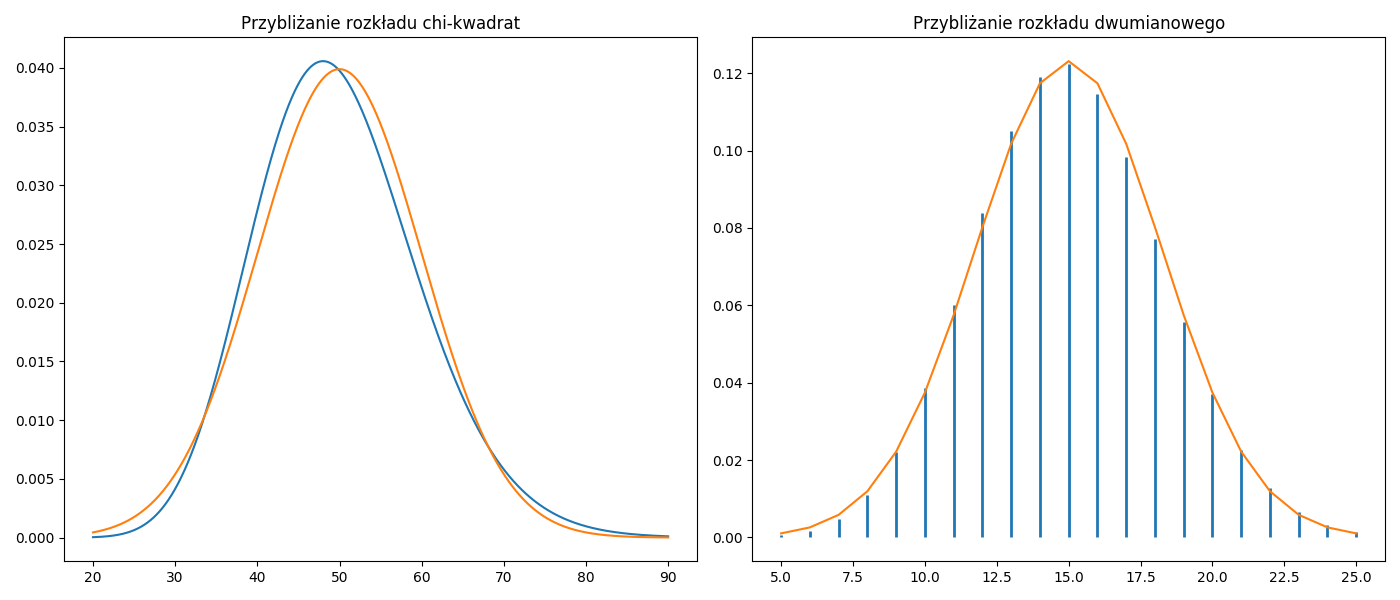
\includegraphics[width=1\linewidth]{plt01} 

}

\caption{Przybliżanie rozkładów.}\label{fig:plt01}
\end{figure}

\hypertarget{R22}{%
\section{Liniowy model regresji}\label{R22}}

Współczynniki modelu liniowego \(Y=\hat{\beta} X+\epsilon\) można znaleźć w stosunkowo prosty sposób wykonując działania na macierzach:
\begin{equation}
\hat{\beta}=(X^{T}X)^{-1}X^{T}Y
\label{eq:n04}
\end{equation}
gdzie \(Y\) to wektor zmiennej zależnej pochodzącej z rozkładu normalnego natomiast \(X\) to macierz zmiennych niezależnych.

Błędy standardowe oszacowanych parametrów to pierwiastki kwadratowe elementów na głównej przekątnej macierzy wariancji i kowariancji:
\begin{equation}
D^2(\hat{\beta})=(X^TX)^{-1}S^2_{e}
\label{eq:n05}
\end{equation}
gdzie \(S^2_e=e^Te/(n-k-1)\) to wariancja reszt i \(e=Y-\hat{\beta}X\) to wektor reszt.

Stopień wyjaśnienia przez model zmiennej zależnej można ocenić za pomocą współczynnika determinacji:
\begin{equation}
R^2=\frac{\sum_{i=1}^{n}(\hat{y}-\bar{y})^2}{\sum_{i=1}^{n}(y-\bar{y})^2}
\label{eq:det}
\end{equation}

Siłę związku dwóch zmiennych można ocenić na podstawie współczynnika korelacji liniowej Pearsona który może być równy pierwiastkowi kwadratowemu współczynnika determinacji ponieważ \(|r|=R\).
\begin{equation}
r=\mathrm{cov}(X,Y)/S_XS_Y
\label{eq:cor}
\end{equation}
gdzie: \(\mathrm{cov}(X,Y)\) to kowariancja dwóch zmiennych natomiast \(S_X\) i \(S_Y\) to odchylenia standardowe zmiennych.

Błąd standardowy korelacji Pearsona dla dużej próby wyznaczamy według wzoru:
\begin{equation}
SE_{r}=\sqrt{(1-r^2)/n}
\label{eq:SEcor}
\end{equation}

Wszystkie wyniki można uzyskać za pomocą funkcji \href{https://docs.scipy.org/doc/scipy/reference/generated/scipy.stats.linregress.html\#scipy.stats.linregress}{\texttt{scipy.stats.linregress}} ale tylko dla jednej zmiennej objaśniającej.

\begin{Shaded}
\begin{Highlighting}[]
\ImportTok{from}\NormalTok{ scipy }\ImportTok{import}\NormalTok{ stats}
\ImportTok{import}\NormalTok{ numpy }\ImportTok{as}\NormalTok{ np}

\NormalTok{x }\OperatorTok{=}\NormalTok{ np.sort(stats.norm.rvs(size}\OperatorTok{=}\DecValTok{300}\NormalTok{,loc}\OperatorTok{=}\DecValTok{3}\NormalTok{,random_state}\OperatorTok{=}\DecValTok{2305}\NormalTok{))}
\NormalTok{y }\OperatorTok{=}\NormalTok{ np.sort(stats.norm.rvs(size}\OperatorTok{=}\DecValTok{300}\NormalTok{,scale}\OperatorTok{=}\DecValTok{3}\NormalTok{,random_state}\OperatorTok{=}\DecValTok{4101}\NormalTok{))}

\NormalTok{beta, const, r_value, p_value, SE_beta }\OperatorTok{=}\NormalTok{ stats.linregress(x, y)}
\NormalTok{SE_r }\OperatorTok{=}\NormalTok{ ((}\DecValTok{1}\OperatorTok{-}\NormalTok{r_value}\OperatorTok{**}\DecValTok{2}\NormalTok{)}\OperatorTok{/}\NormalTok{(}\BuiltInTok{len}\NormalTok{(x)))}\OperatorTok{**}\FloatTok{0.5}
\BuiltInTok{print}\NormalTok{(}\StringTok{"beta: }\SpecialCharTok{%f}\StringTok{, SE_beta: }\SpecialCharTok\NormalTok{ (beta,SE_beta))}
\BuiltInTok{print}\NormalTok{(}\StringTok{"cor: }\SpecialCharTok{%f}\StringTok{, SE_cor: }\SpecialCharTok\NormalTok{ (r_value,SE_r))}
\end{Highlighting}
\end{Shaded}

\begin{verbatim}
## beta: 2.820229, SE_beta: 0.009932
## cor: 0.998157, SE_cor: 0.003503
\end{verbatim}

Przedstawiona powyżej procedura szacowania parametrów to metoda najmniejszych kwadratów która minimalizuje sumę kwadratów reszt:
\begin{equation}
RSS=e^Te\quad\longrightarrow\quad\mbox{min}
\label{eq:n06}
\end{equation}
Innym kryterium optymalizacji możne być maksymalizacja logarytmu wiarygodności:
\begin{equation}
LL=-\frac{n}{2}\ln(2\pi\sigma^2)-\frac{e^Te}{2\sigma^2}\quad\longrightarrow\quad\mbox{max}
\label{eq:n07}
\end{equation}
Obie procedury: metoda najmniejszych kwadratów \eqref{eq:n06} i metoda największej wiarygodności \eqref{eq:n07} dla dowolnej liczby zmiennych objaśniających zostały udostępnione w pakiecie \href{https://www.statsmodels.org/stable/examples/index.html\#regression}{\texttt{statsmodels}}.
Ciekawą alternatywą jest wykorzystanie algorytmów optymalizacyjnych ogólnego przeznaczenia z pakietu \href{https://docs.scipy.org/doc/scipy/reference/generated/scipy.optimize.minimize.html\#scipy.optimize.minimize}{\texttt{scipy.optimize.minimize}}. Takie rozwiązanie (patrz podrozdział \ref{R33}) umożliwia szacowanie parametrów modeli o dowolnej postaci analitycznej po uprzednim zdefiniowaniu funkcji logarytmu wiarygodności.

\begin{Shaded}
\begin{Highlighting}[]
\ImportTok{from}\NormalTok{ scipy }\ImportTok{import}\NormalTok{ stats}
\ImportTok{import}\NormalTok{ numpy }\ImportTok{as}\NormalTok{ np}
\ImportTok{import}\NormalTok{ pandas }\ImportTok{as}\NormalTok{ pd}

\NormalTok{df }\OperatorTok{=}\NormalTok{ pd.DataFrame(data}\OperatorTok{=}\NormalTok{\{}\StringTok{'x'}\NormalTok{:np.sort(stats.norm.rvs(size}\OperatorTok{=}\DecValTok{300}\NormalTok{,loc}\OperatorTok{=}\DecValTok{3}\NormalTok{,random_state}\OperatorTok{=}\DecValTok{2305}\NormalTok{)),}
                        \StringTok{'y'}\NormalTok{:np.sort(stats.norm.rvs(size}\OperatorTok{=}\DecValTok{300}\NormalTok{,scale}\OperatorTok{=}\DecValTok{3}\NormalTok{,random_state}\OperatorTok{=}\DecValTok{4101}\NormalTok{))\})}

\ImportTok{import}\NormalTok{ statsmodels.formula.api }\ImportTok{as}\NormalTok{ smf}

\NormalTok{m }\OperatorTok{=}\NormalTok{ smf.ols(}\StringTok{"y~x"}\NormalTok{, data}\OperatorTok{=}\NormalTok{df).fit()}
\BuiltInTok{print}\NormalTok{(m.summary())}
\end{Highlighting}
\end{Shaded}

\begin{verbatim}
##                             OLS Regression Results                            
## ==============================================================================
## Dep. Variable:                      y   R-squared:                       0.996
## Model:                            OLS   Adj. R-squared:                  0.996
## Method:                 Least Squares   F-statistic:                 8.064e+04
## Date:                Mon, 19 Aug 2019   Prob (F-statistic):               0.00
## Time:                        19:22:53   Log-Likelihood:                 99.901
## No. Observations:                 300   AIC:                            -195.8
## Df Residuals:                     298   BIC:                            -188.4
## Df Model:                           1                                         
## Covariance Type:            nonrobust                                         
## ==============================================================================
##                  coef    std err          t      P>|t|      [0.025      0.975]
## ------------------------------------------------------------------------------
## Intercept     -8.2571      0.032   -260.743      0.000      -8.319      -8.195
## x              2.8202      0.010    283.964      0.000       2.801       2.840
## ==============================================================================
## Omnibus:                       29.693   Durbin-Watson:                   0.280
## Prob(Omnibus):                  0.000   Jarque-Bera (JB):              127.091
## Skew:                           0.201   Prob(JB):                     2.53e-28
## Kurtosis:                       6.163   Cond. No.                         10.9
## ==============================================================================
## 
## Warnings:
## [1] Standard Errors assume that the covariance matrix of the errors is correctly specified.
\end{verbatim}

\hypertarget{R23}{%
\section{Nieliniowy model regresji}\label{R23}}

Jeśli badana zależność ma charakter nieliniowy a zmienna objaśniana pochodzi z rozkładu normalnego to można zastosować nieliniową metodę najmniejszych kwadratów np. algorytm Levenberga-Marquardta lub Trust Region Reflective jeśli chcemy dodać ograniczenia przedziałowe na parametry. Obie procedury zostały zaimplementowane do funkcji
\href{https://docs.scipy.org/doc/scipy/reference/generated/scipy.optimize.curve_fit.html}{\texttt{scipy.optimize.curve\_fit}}. Dodajmy jeszcze, że są to procedury iteracyjne które wymagają określenia parametrów startowych. W pewnych sytuacjach można je wyznaczyć za pomocą tzw. linearyzacji czyli po sprowadzeniu modelu nieliniowego do postaci liniowej ale nie zawsze jest to możliwe. Poniżej przykłady linearyzacji wybranych modeli nieliniowych:

\begin{itemize}
\tightlist
\item
  model potęgowy:
\end{itemize}

\begin{equation}
y=a\cdot x^b \quad \longrightarrow \quad \ln(y)=\alpha+\beta\cdot \ln(x)\quad \longrightarrow \quad \exp(\alpha)= a,\quad \beta=b
\label{eq:n08}
\end{equation}

\begin{itemize}
\tightlist
\item
  model Tornquista 1:
\end{itemize}

\begin{equation}
y=\frac{ax}{x+b} \quad \longrightarrow \quad \frac{1}{y}=\alpha+\beta\cdot \frac{1}{x}\quad \longrightarrow \quad \frac{1}{\alpha}= a,\quad \frac{\beta}{\alpha}=b
\label{eq:n09}
\end{equation}

\begin{Shaded}
\begin{Highlighting}[]
\ImportTok{import}\NormalTok{ scipy.stats }\ImportTok{as}\NormalTok{ stats}
\ImportTok{import}\NormalTok{ matplotlib.pyplot }\ImportTok{as}\NormalTok{ plt}
\ImportTok{import}\NormalTok{ statsmodels.formula.api }\ImportTok{as}\NormalTok{ smf}
\ImportTok{import}\NormalTok{ numpy }\ImportTok{as}\NormalTok{ np}
\ImportTok{import}\NormalTok{ pandas }\ImportTok{as}\NormalTok{ pd}
\ImportTok{from}\NormalTok{ scipy.optimize }\ImportTok{import}\NormalTok{ curve_fit}

\NormalTok{x }\OperatorTok{=}\NormalTok{ stats.uniform.rvs(}\DecValTok{1}\NormalTok{,}\DecValTok{10}\NormalTok{,size}\OperatorTok{=}\DecValTok{100}\NormalTok{, random_state}\OperatorTok{=}\DecValTok{2305}\NormalTok{)}
\NormalTok{mu }\OperatorTok{=} \FloatTok{20.8} \OperatorTok{*}\NormalTok{ x}\OperatorTok{**}\FloatTok{0.45}
\NormalTok{y }\OperatorTok{=}\NormalTok{ stats.norm.rvs(loc}\OperatorTok{=}\NormalTok{mu,scale}\OperatorTok{=}\DecValTok{1}\NormalTok{,size}\OperatorTok{=}\DecValTok{100}\NormalTok{,random_state}\OperatorTok{=}\DecValTok{2305}\NormalTok{)}
\NormalTok{lx }\OperatorTok{=}\NormalTok{ np.log(x)}
\NormalTok{ly }\OperatorTok{=}\NormalTok{ np.log(y)}
\NormalTok{df }\OperatorTok{=}\NormalTok{ pd.DataFrame(\{}\StringTok{'x'}\NormalTok{:x,}\StringTok{'y'}\NormalTok{:y,}\StringTok{'lx'}\NormalTok{:lx,}\StringTok{'ly'}\NormalTok{:ly\})}

\NormalTok{modLog }\OperatorTok{=}\NormalTok{ smf.glm(}\StringTok{'ly~lx'}\NormalTok{, data}\OperatorTok{=}\NormalTok{df).fit()}
\NormalTok{p }\OperatorTok{=}\NormalTok{ modLog.params.values}
\NormalTok{pse }\OperatorTok{=}\NormalTok{ np.diag(modLog.cov_params())}\OperatorTok{**}\FloatTok{0.5}

\KeywordTok{def}\NormalTok{ modNLS(x,a,b):}
    \ControlFlowTok{return}\NormalTok{ a}\OperatorTok{*}\NormalTok{x}\OperatorTok{**}\NormalTok{b}

\NormalTok{sol, pcov }\OperatorTok{=}\NormalTok{ curve_fit(modNLS, x, y, p0}\OperatorTok{=}\NormalTok{(np.exp(p[}\DecValTok{0}\NormalTok{]),p[}\DecValTok{1}\NormalTok{]))}
\NormalTok{se }\OperatorTok{=}\NormalTok{ np.diag(pcov)}\OperatorTok{**}\FloatTok{0.5}

\NormalTok{fig }\OperatorTok{=}\NormalTok{ plt.figure(figsize}\OperatorTok{=}\NormalTok{(}\DecValTok{14}\NormalTok{,}\DecValTok{6}\NormalTok{))}
\NormalTok{ax1 }\OperatorTok{=}\NormalTok{ fig.add_subplot(}\DecValTok{1}\NormalTok{,}\DecValTok{2}\NormalTok{,}\DecValTok{1}\NormalTok{)}
\NormalTok{ax2 }\OperatorTok{=}\NormalTok{ fig.add_subplot(}\DecValTok{1}\NormalTok{,}\DecValTok{2}\NormalTok{,}\DecValTok{2}\NormalTok{)}
\NormalTok{lX }\OperatorTok{=}\NormalTok{ np.linspace(np.}\BuiltInTok{min}\NormalTok{(lx),np.}\BuiltInTok{max}\NormalTok{(lx), }\DecValTok{500}\NormalTok{)}
\NormalTok{ax1.plot(lX,p[}\DecValTok{0}\NormalTok{]}\OperatorTok{+}\NormalTok{p[}\DecValTok{1}\NormalTok{]}\OperatorTok{*}\NormalTok{lX,}
\NormalTok{         label}\OperatorTok{=}\StringTok{'$}\CharTok{\textbackslash{}\textbackslash{}}\StringTok{alpha$ = }\SpecialCharTok{%.2f}\StringTok{ (se: }\SpecialCharTok{%.4f}\StringTok{), $}\CharTok{\textbackslash{}\textbackslash{}}\StringTok{beta$ = }\SpecialCharTok{%.2f}\StringTok{ (se: }\SpecialCharTok\NormalTok{ (p[}\DecValTok{0}\NormalTok{],pse[}\DecValTok{0}\NormalTok{],p[}\DecValTok{1}\NormalTok{],pse[}\DecValTok{1}\NormalTok{]))}
\NormalTok{ax1.plot(lx,ly,}\StringTok{'o'}\NormalTok{,alpha}\OperatorTok{=}\FloatTok{0.5}\NormalTok{,label}\OperatorTok{=}\StringTok{'log dane'}\NormalTok{)}
\NormalTok{ax1.set_xlabel(}\StringTok{"log x"}\NormalTok{)}
\NormalTok{ax1.set_ylabel(}\StringTok{"log y"}\NormalTok{)}
\NormalTok{ax1.legend()}
\NormalTok{ax1.set_title(}\StringTok{"Liniowa metoda najmniejszych kwadratów\textbackslash{}n$}\CharTok{\textbackslash{}\textbackslash{}}\StringTok{ln(y)=}\CharTok{\textbackslash{}\textbackslash{}}\StringTok{alpha+}\CharTok{\textbackslash{}\textbackslash{}}\StringTok{beta}\CharTok{\textbackslash{}\textbackslash{}}\StringTok{ln(x)$"}\NormalTok{)}
\NormalTok{X }\OperatorTok{=}\NormalTok{ np.linspace(np.}\BuiltInTok{min}\NormalTok{(x),np.}\BuiltInTok{max}\NormalTok{(x), }\DecValTok{500}\NormalTok{)}
\NormalTok{ax2.plot(X,modNLS(X,sol[}\DecValTok{0}\NormalTok{],sol[}\DecValTok{1}\NormalTok{]),}
\NormalTok{         label}\OperatorTok{=}\StringTok{'a = }\SpecialCharTok{%.2f}\StringTok{ (se: }\SpecialCharTok{%.4f}\StringTok{), b= }\SpecialCharTok{%.2f}\StringTok{ (se: }\SpecialCharTok\NormalTok{ (sol[}\DecValTok{0}\NormalTok{],se[}\DecValTok{0}\NormalTok{],sol[}\DecValTok{1}\NormalTok{],se[}\DecValTok{1}\NormalTok{]))}
\NormalTok{ax2.plot(x,y,}\StringTok{'o'}\NormalTok{,alpha}\OperatorTok{=}\FloatTok{0.5}\NormalTok{,label}\OperatorTok{=}\StringTok{'dane'}\NormalTok{)}
\NormalTok{ax2.set_title(}\StringTok{"Nieliniowa metoda najmniejszych kwadratów\textbackslash{}n$y=ax^b$"}\NormalTok{)}
\NormalTok{ax2.set_xlabel(}\StringTok{"x"}\NormalTok{)}
\NormalTok{ax2.set_ylabel(}\StringTok{"y"}\NormalTok{)}
\NormalTok{ax2.legend()}
\NormalTok{fig.tight_layout()}
\NormalTok{plt.savefig(}\StringTok{'modlin01.png'}\NormalTok{)}
\end{Highlighting}
\end{Shaded}

\begin{figure}[h]

{\centering 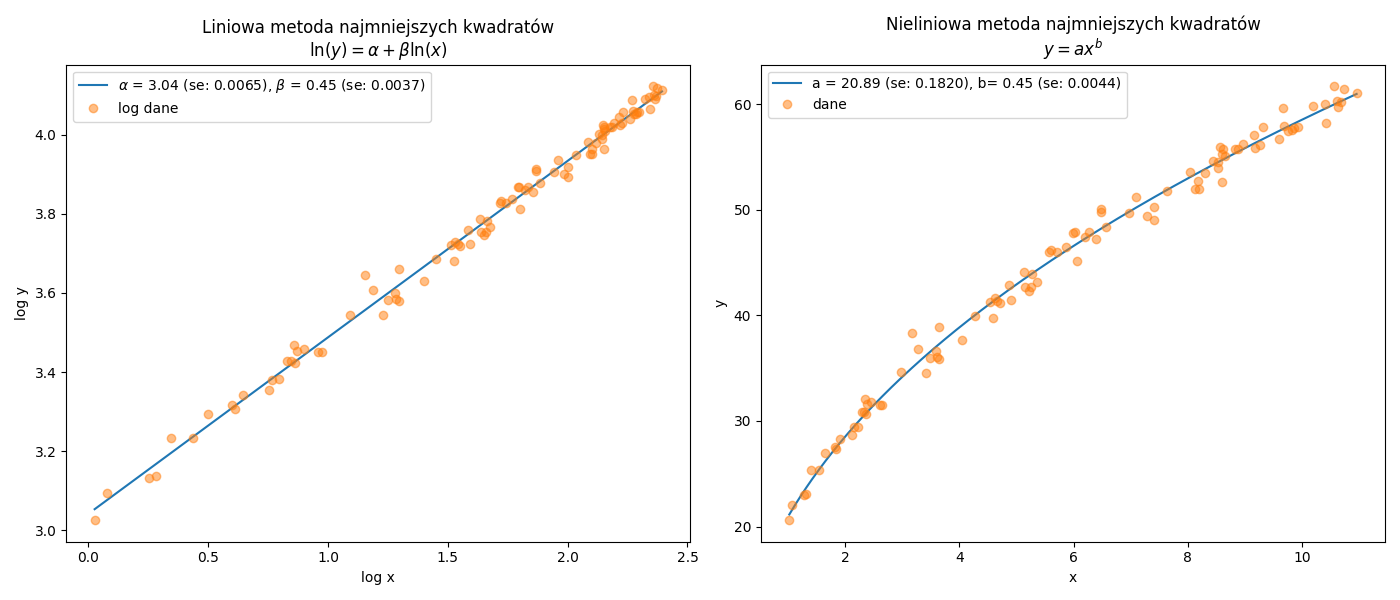
\includegraphics[width=1\linewidth]{modlin01} 

}

\caption{Graficzna prezentacja linearyzacji funkcji nieliniowej.}\label{fig:modlin01}
\end{figure}

Alternatywnym rozwiązaniem jest metoda największej wiarygodności w której można założyć dowolny rozkład prawdopodobieństwa dla zmiennej zależnej. Ta metoda jest stosowana do estymacji parametrów uogólnionych modeli liniowych w których trzeba określić rozkład z rodziny rozkładów wykładniczych dla zmiennej objaśnianej. Dodatkowo dzięki funkcji wiążącej można rozpatrywać szególne przypadki powiązania zmiennej objaśniającej z predyktorem. Przykładowo dla rozkładu normalnego domyślnie jest estymowany model liniowy - opcja \texttt{identity}: \(\hat{\mu}=\hat{y}\) ale możliwe są też takie przypadki jak \texttt{inverse\_power}: \(\hat{\mu}=1/\hat{y}\) oraz \texttt{log}: \(\hat{\mu}=\exp(\hat{y})\) gdzie \(\hat{y}=\beta_0+\sum_{j=1}^{n}\beta_j x_{ij}\). Warto zaznaczyć, że
średnia na skali logarytmicznej nie jest równa logarytmowi średniej na oryginalnej skali tzn.
\(E(\ln Y_i)\neq \ln E(Y_i)\).

\begin{Shaded}
\begin{Highlighting}[]
\ImportTok{import}\NormalTok{ scipy.stats }\ImportTok{as}\NormalTok{ stats}
\ImportTok{import}\NormalTok{ matplotlib.pyplot }\ImportTok{as}\NormalTok{ plt}
\ImportTok{import}\NormalTok{ statsmodels.formula.api }\ImportTok{as}\NormalTok{ smf}
\ImportTok{import}\NormalTok{ statsmodels.api }\ImportTok{as}\NormalTok{ sm}
\ImportTok{import}\NormalTok{ numpy }\ImportTok{as}\NormalTok{ np}
\ImportTok{import}\NormalTok{ pandas }\ImportTok{as}\NormalTok{ pd}
\ImportTok{from}\NormalTok{ scipy.optimize }\ImportTok{import}\NormalTok{ curve_fit}

\NormalTok{x }\OperatorTok{=}\NormalTok{ stats.uniform.rvs(}\DecValTok{1}\NormalTok{,}\DecValTok{7}\NormalTok{,size}\OperatorTok{=}\DecValTok{100}\NormalTok{, random_state}\OperatorTok{=}\DecValTok{2305}\NormalTok{)}
\NormalTok{mu }\OperatorTok{=} \DecValTok{1}\OperatorTok{/}\NormalTok{(}\FloatTok{1.25+8.25}\OperatorTok{*}\NormalTok{x)}
\NormalTok{MU }\OperatorTok{=}\NormalTok{ np.exp(}\FloatTok{3.25+0.88}\OperatorTok{*}\NormalTok{x)}
\NormalTok{y }\OperatorTok{=}\NormalTok{ stats.norm.rvs(loc}\OperatorTok{=}\NormalTok{mu,scale}\OperatorTok{=}\FloatTok{0.0025}\NormalTok{,size}\OperatorTok{=}\DecValTok{100}\NormalTok{,random_state}\OperatorTok{=}\DecValTok{2305}\NormalTok{)}
\NormalTok{z }\OperatorTok{=}\NormalTok{ MU}\OperatorTok{+}\NormalTok{stats.norm.rvs(scale}\OperatorTok{=}\DecValTok{200}\NormalTok{,size}\OperatorTok{=}\DecValTok{100}\NormalTok{,random_state}\OperatorTok{=}\DecValTok{2305}\NormalTok{)}
\NormalTok{X }\OperatorTok{=}\NormalTok{ np.linspace(np.}\BuiltInTok{min}\NormalTok{(x),np.}\BuiltInTok{max}\NormalTok{(x), }\DecValTok{500}\NormalTok{)}
  
\NormalTok{gaus1 }\OperatorTok{=}\NormalTok{ smf.glm(}\StringTok{'y~x'}\NormalTok{, data}\OperatorTok{=}\NormalTok{pd.DataFrame(\{}\StringTok{'x'}\NormalTok{:x,}\StringTok{'y'}\NormalTok{:y\}),}\OperatorTok{\textbackslash{}}
\NormalTok{        family}\OperatorTok{=}\NormalTok{sm.families.Gaussian(sm.families.links.inverse_power)).fit()}
\NormalTok{p }\OperatorTok{=}\NormalTok{ gaus1.params.values}
\NormalTok{pSE }\OperatorTok{=}\NormalTok{ np.diag(gaus1.cov_params())}\OperatorTok{**}\FloatTok{0.5}
\NormalTok{gaus2 }\OperatorTok{=}\NormalTok{ smf.glm(}\StringTok{'z~x'}\NormalTok{, data}\OperatorTok{=}\NormalTok{pd.DataFrame(\{}\StringTok{'x'}\NormalTok{:x,}\StringTok{'z'}\NormalTok{:z\}),}\OperatorTok{\textbackslash{}}
\NormalTok{        family}\OperatorTok{=}\NormalTok{sm.families.Gaussian(sm.families.links.log)).fit()}
\NormalTok{P }\OperatorTok{=}\NormalTok{ gaus2.params.values}
\NormalTok{Pse }\OperatorTok{=}\NormalTok{ np.diag(gaus2.cov_params())}\OperatorTok{**}\FloatTok{0.5}
\BuiltInTok{print}\NormalTok{(}\StringTok{"GLM: family=Gaussian, link='inverse_power'"}\NormalTok{)}
\BuiltInTok{print}\NormalTok{(gaus1.summary().tables[}\DecValTok{1}\NormalTok{])}
\BuiltInTok{print}\NormalTok{(}\StringTok{"}\CharTok{\textbackslash{}n}\StringTok{GLM: family=Gaussian, link='log'"}\NormalTok{)}
\BuiltInTok{print}\NormalTok{(gaus2.summary().tables[}\DecValTok{1}\NormalTok{])}

\NormalTok{fig }\OperatorTok{=}\NormalTok{ plt.figure(figsize}\OperatorTok{=}\NormalTok{(}\DecValTok{14}\NormalTok{,}\DecValTok{6}\NormalTok{))}
\NormalTok{ax1 }\OperatorTok{=}\NormalTok{ fig.add_subplot(}\DecValTok{1}\NormalTok{,}\DecValTok{2}\NormalTok{,}\DecValTok{1}\NormalTok{)}
\NormalTok{ax2 }\OperatorTok{=}\NormalTok{ fig.add_subplot(}\DecValTok{1}\NormalTok{,}\DecValTok{2}\NormalTok{,}\DecValTok{2}\NormalTok{)}
\NormalTok{ax1.plot(X, }\DecValTok{1}\OperatorTok{/}\NormalTok{(p[}\DecValTok{0}\NormalTok{]}\OperatorTok{+}\NormalTok{p[}\DecValTok{1}\NormalTok{]}\OperatorTok{*}\NormalTok{X),label}\OperatorTok{=}\StringTok{'a = }\SpecialCharTok{%.4f}\StringTok{, b= }\SpecialCharTok\NormalTok{ (p[}\DecValTok{0}\NormalTok{],p[}\DecValTok{1}\NormalTok{]))}
\NormalTok{ax1.plot(x,y,}\StringTok{'o'}\NormalTok{,alpha}\OperatorTok{=}\FloatTok{0.5}\NormalTok{,label}\OperatorTok{=}\StringTok{"y"}\NormalTok{)         }
\NormalTok{ax1.set_title(}\StringTok{"GLM: family=Gaussian, link='inverse_power'}\CharTok{\textbackslash{}n}\StringTok{ $}\CharTok{\textbackslash{}\textbackslash{}}\StringTok{hat\{}\CharTok{\textbackslash{}\textbackslash{}}\StringTok{mu\}=}\CharTok{\textbackslash{}\textbackslash{}}\StringTok{frac}\SpecialCharTok{\{1\}}\StringTok{\{a+bx\}$"}\NormalTok{)}
\NormalTok{ax1.legend()}
\NormalTok{ax2.plot(X, np.exp(P[}\DecValTok{0}\NormalTok{]}\OperatorTok{+}\NormalTok{P[}\DecValTok{1}\NormalTok{]}\OperatorTok{*}\NormalTok{X),label}\OperatorTok{=}\StringTok{'a = }\SpecialCharTok{%.4f}\StringTok{, b= }\SpecialCharTok\NormalTok{ (P[}\DecValTok{0}\NormalTok{],P[}\DecValTok{1}\NormalTok{]))}
\NormalTok{ax2.plot(x,z,}\StringTok{'o'}\NormalTok{,alpha}\OperatorTok{=}\FloatTok{0.5}\NormalTok{,label}\OperatorTok{=}\StringTok{'z'}\NormalTok{)}
\NormalTok{ax2.set_title(}\StringTok{"GLM: family=Gaussian, link='log'}\CharTok{\textbackslash{}n}\StringTok{ $}\CharTok{\textbackslash{}\textbackslash{}}\StringTok{hat\{}\CharTok{\textbackslash{}\textbackslash{}}\StringTok{mu\}=}\CharTok{\textbackslash{}\textbackslash{}}\StringTok{exp(a+bx)$"}\NormalTok{)}
\NormalTok{ax2.legend()}
\NormalTok{fig.tight_layout()}
\NormalTok{plt.savefig(}\StringTok{'modlin02.png'}\NormalTok{)}
\end{Highlighting}
\end{Shaded}

\begin{verbatim}
## GLM: family=Gaussian, link='inverse_power'
## ==============================================================================
##                  coef    std err          z      P>|z|      [0.025      0.975]
## ------------------------------------------------------------------------------
## Intercept      1.1263      0.214      5.275      0.000       0.708       1.545
## x              8.2971      0.127     65.083      0.000       8.047       8.547
## ==============================================================================
## 
## GLM: family=Gaussian, link='log'
## ==============================================================================
##                  coef    std err          z      P>|z|      [0.025      0.975]
## ------------------------------------------------------------------------------
## Intercept      3.2250      0.030    106.185      0.000       3.165       3.285
## x              0.8834      0.004    216.194      0.000       0.875       0.891
## ==============================================================================
\end{verbatim}

\begin{figure}[h]

{\centering 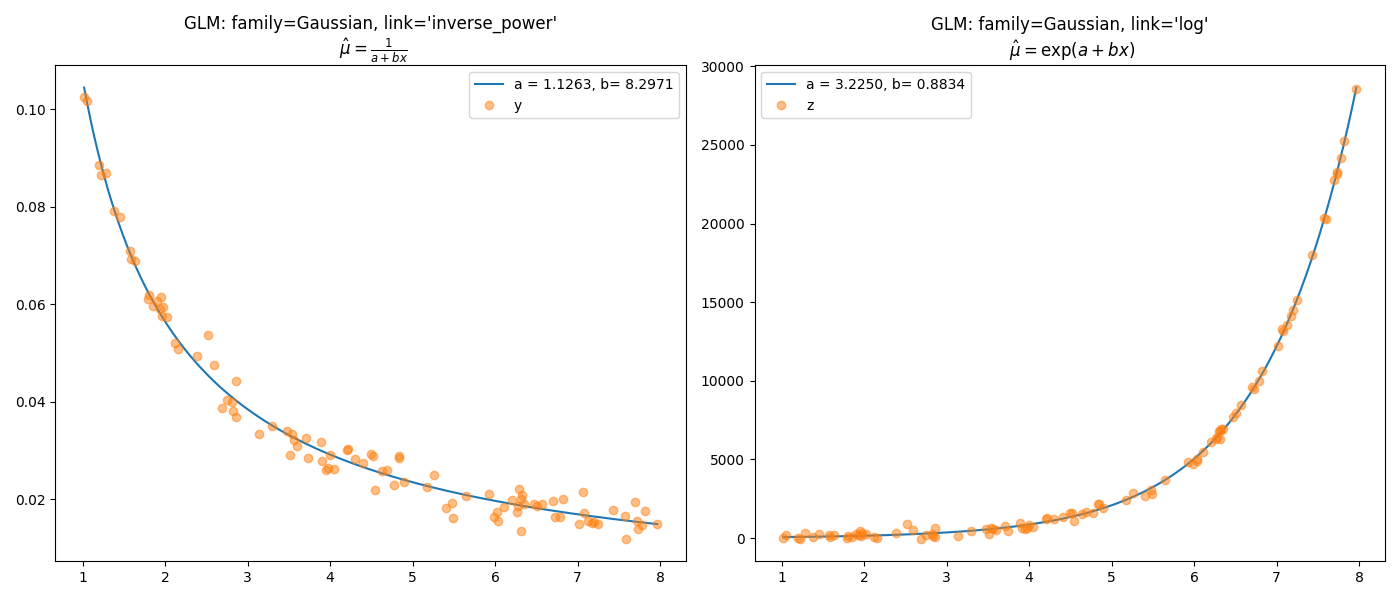
\includegraphics[width=1\linewidth]{modlin02} 

}

\caption{Graficzna prezentacja dwóch funkcji wiążących z wykorzystaniem rozkładu Gaussa.}\label{fig:modlin02}
\end{figure}

\hypertarget{R3}{%
\chapter{Rozkład gamma}\label{R3}}

\begin{center}\rule{0.5\linewidth}{\linethickness}\end{center}

\hypertarget{R31}{%
\section{Funkcja gęstości}\label{R31}}

Uogólniony rozkład gamma zaimplementowany do funkcji \href{https://docs.scipy.org/doc/scipy/reference/generated/scipy.stats.gengamma.html\#scipy.stats.gengamma}{\texttt{scipy.stats.gengamma.pdf}} można przedstawić za pomocą wzoru:
\begin{equation}
f(x\;|\;a,k,m,s)=\frac{k(x-m)^{ka-1}}{s^{ka}\Gamma(a)}\exp\left(-\left(\frac{x-m}{s}\right)^k\right)
\label{eq:g01}
\end{equation}
gdzie \(k\neq 0\) i \(a>0\) to parametry kształtu (shape), \(s>0\) to parametr skali (scale) oraz \(m\) to parametr przesunięcia.
Przypadek dla \(k=1\) został zaimplementowany do funkcji \href{https://docs.scipy.org/doc/scipy/reference/generated/scipy.stats.gamma.html}{\texttt{scipy.stats.gamma.pdf}} jako trójparametrowa wersja rozkładu gamma która jest dana wzorem:
\begin{equation}
f(x\;|\;a,m,s)=\frac{(x-m)^{a-1}}{s^{a}\Gamma(a)}\exp\left(-\frac{x-m}{s}\right)
\label{eq:g02}
\end{equation}

Jeśli będziemy rozważać dwuparametrowy rozkład gamma tzn. z pominięciem parametru przesunięcia czyli \(m=0\) to wtedy wzór rozkładu uprości się do postaci:
\begin{equation}
f(x\;|\;a,s)=\frac{x^{a-1}}{s^{a}\Gamma(a)}\exp\left(-\frac{x}{s}\right)\quad\mbox{gdzie}\quad E(X)=as,\; V(X)=as^2
\label{eq:g03}
\end{equation}
W innej implementacji tego rozkładu zamiast parametru skali \(s\) (scale) jest stosowany parametr \(r\) (rate) gdzie \(r = 1 / s\):
\begin{equation}
f(x\;|\;a,r)=\frac{r^ax^{a-1}}{\Gamma(a)}\exp(-rx)\quad\mbox{gdzie}\quad E(X)=a/r,\; V(X)=a/r^2
\label{eq:g04}
\end{equation}

Do estymacji parametrów rozkładu można wykorzystać metodę największej wiarygodności która polega na optymalizacji zlogarytmowanej funkcji wiarygodności:
\begin{align}
     LL_{scale} & =(a-1)\ln(y)-(y/s)-a\ln(s)-\ln\Gamma(a) \label{eq:g05}\\
     LL_{rate} & =a\ln(ry)-\ln\Gamma(a)-\ln(y)-ry \label{eq:g06}
  \end{align}

Funkcja \href{https://docs.scipy.org/doc/scipy/reference/generated/scipy.stats.gamma.html\#scipy.stats.gamma}{\texttt{scipy.stats.gamma.fit}} wykonuje estymację parametrów: \(a\), \(m\) oraz \(s\). Dzięki argumentom \texttt{floc}, \texttt{fscale} i \texttt{fa} możemy założyć stałą wartość dwóch lub jednego parametru. Jeśli założymy, że \(m=0\) to będziemy optymalizować funkcję \eqref{eq:g05} czyli oszacujemy parametr kształtu \(a\) oraz skali \(s\).

\begin{Shaded}
\begin{Highlighting}[]
\ImportTok{import}\NormalTok{ scipy.stats }\ImportTok{as}\NormalTok{ stats}
\ImportTok{import}\NormalTok{ matplotlib.pyplot }\ImportTok{as}\NormalTok{ plt}
\ImportTok{import}\NormalTok{ statsmodels.api }\ImportTok{as}\NormalTok{ sm}

\NormalTok{y }\OperatorTok{=}\NormalTok{ stats.gamma.rvs(}\FloatTok{2.83}\NormalTok{, size}\OperatorTok{=}\DecValTok{100}\NormalTok{, random_state}\OperatorTok{=}\DecValTok{2305}\NormalTok{)}
\NormalTok{f }\OperatorTok{=}\NormalTok{ stats.gamma.fit(y)}
\NormalTok{F }\OperatorTok{=}\NormalTok{ stats.gengamma.fit(y)}
\NormalTok{logLik_f }\OperatorTok{=} \BuiltInTok{sum}\NormalTok{(stats.gamma.logpdf(y, a}\OperatorTok{=}\NormalTok{f[}\DecValTok{0}\NormalTok{], loc}\OperatorTok{=}\NormalTok{f[}\DecValTok{1}\NormalTok{], scale}\OperatorTok{=}\NormalTok{f[}\DecValTok{2}\NormalTok{]))}
\NormalTok{logLik_F }\OperatorTok{=} \BuiltInTok{sum}\NormalTok{(stats.gengamma.logpdf(y, a}\OperatorTok{=}\NormalTok{F[}\DecValTok{0}\NormalTok{], c}\OperatorTok{=}\NormalTok{F[}\DecValTok{1}\NormalTok{], loc}\OperatorTok{=}\NormalTok{F[}\DecValTok{2}\NormalTok{], scale}\OperatorTok{=}\NormalTok{F[}\DecValTok{3}\NormalTok{]))}
    
\NormalTok{fig }\OperatorTok{=}\NormalTok{ plt.figure(figsize}\OperatorTok{=}\NormalTok{(}\DecValTok{14}\NormalTok{,}\DecValTok{6}\NormalTok{))}
\NormalTok{ax1 }\OperatorTok{=}\NormalTok{ fig.add_subplot(}\DecValTok{1}\NormalTok{,}\DecValTok{2}\NormalTok{,}\DecValTok{1}\NormalTok{)}
\NormalTok{ax2 }\OperatorTok{=}\NormalTok{ fig.add_subplot(}\DecValTok{1}\NormalTok{,}\DecValTok{2}\NormalTok{,}\DecValTok{2}\NormalTok{)}
\NormalTok{sm.qqplot(y, stats.gamma, fit}\OperatorTok{=}\VariableTok{True}\NormalTok{, line}\OperatorTok{=}\StringTok{'45'}\NormalTok{, alpha}\OperatorTok{=}\FloatTok{0.25}\NormalTok{, ax}\OperatorTok{=}\NormalTok{ax1)}
\NormalTok{sm.qqplot(y, stats.gengamma, fit}\OperatorTok{=}\VariableTok{True}\NormalTok{, line}\OperatorTok{=}\StringTok{'45'}\NormalTok{, alpha}\OperatorTok{=}\FloatTok{0.25}\NormalTok{, ax}\OperatorTok{=}\NormalTok{ax2)}
\NormalTok{ax1.set_title(}\StringTok{"Rozkład gamma: a= }\SpecialCharTok{%.4f}\StringTok{, loc= }\SpecialCharTok{%.4f}\StringTok{, scale= }\SpecialCharTok{%.4f}\CharTok{\textbackslash{}n}\StringTok{ logLik= }\SpecialCharTok\NormalTok{ (f[}\DecValTok{0}\NormalTok{],f[}\DecValTok{1}\NormalTok{],f[}\DecValTok{2}\NormalTok{],logLik_f))}
\NormalTok{ax2.set_title(}\StringTok{"Uogólniony rozkład gamma: a= }\SpecialCharTok{%.4f}\StringTok{, k= }\SpecialCharTok{%.4f}\StringTok{, loc= }\SpecialCharTok{%.4f}\StringTok{, scale= }\SpecialCharTok{%.4f}\CharTok{\textbackslash{}n}\StringTok{ logLik= }\SpecialCharTok\NormalTok{ (F[}\DecValTok{0}\NormalTok{],F[}\DecValTok{1}\NormalTok{],F[}\DecValTok{2}\NormalTok{],F[}\DecValTok{3}\NormalTok{],logLik_F))}
\NormalTok{fig.tight_layout()}
\NormalTok{plt.savefig(}\StringTok{'gamma01.png'}\NormalTok{)}
\end{Highlighting}
\end{Shaded}

\begin{figure}[h]

{\centering 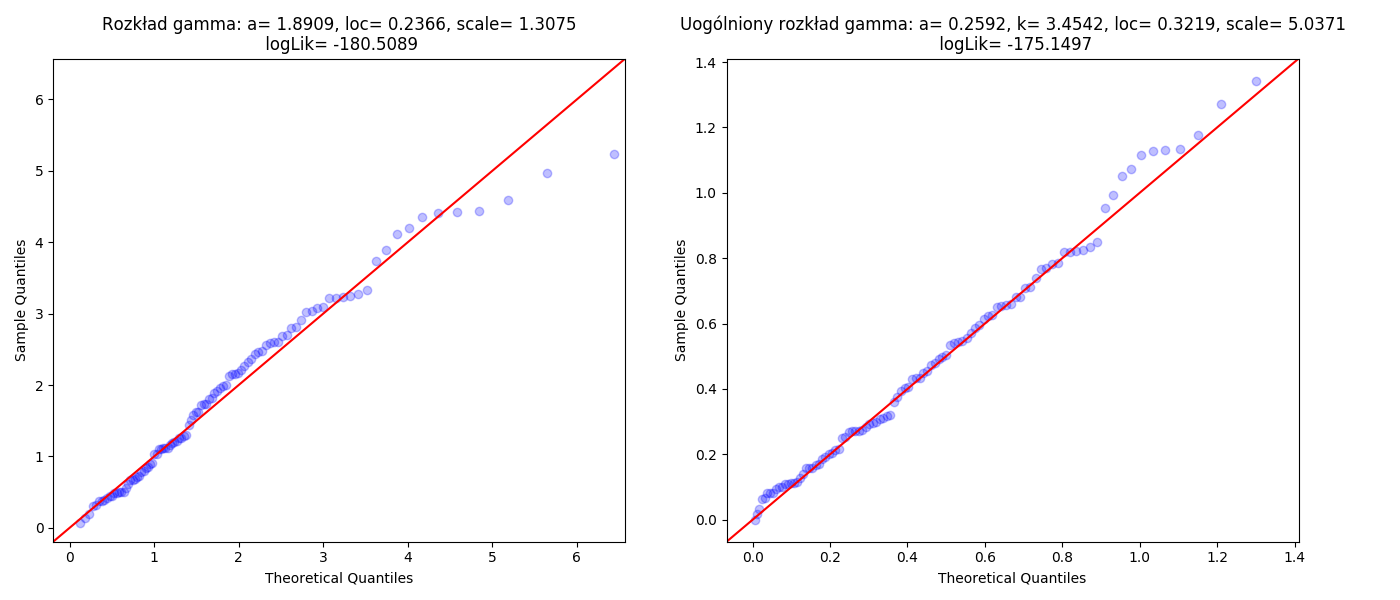
\includegraphics[width=1\linewidth]{gamma01} 

}

\caption{Wykresy kwantylowe.}\label{fig:gamma01}
\end{figure}

\hypertarget{R32}{%
\section{Liniowy model gamma regresji}\label{R32}}

Metoda najmniejszych kwadratów ma zastosowanie w modelowaniu zmiennej objaśnianej która pochodzi z rozkładu normalnego. Zatem gdy zmienna zależna przyjmuje tylko nieujemne wartości z rozkładu ciągłego prawostronnie skośnego to warto rozważyć zastosowanie uogólnionego modelu liniowego z rozkładem gamma i logarytmiczną funkcją wiążącą.

\begin{Shaded}
\begin{Highlighting}[]
\ImportTok{import}\NormalTok{ scipy.stats }\ImportTok{as}\NormalTok{ stats}
\ImportTok{import}\NormalTok{ matplotlib.pyplot }\ImportTok{as}\NormalTok{ plt}
\ImportTok{import}\NormalTok{ statsmodels.api }\ImportTok{as}\NormalTok{ sm}
\ImportTok{import}\NormalTok{ statsmodels.formula.api }\ImportTok{as}\NormalTok{ smf}
\ImportTok{import}\NormalTok{ numpy }\ImportTok{as}\NormalTok{ np}
\ImportTok{import}\NormalTok{ pandas }\ImportTok{as}\NormalTok{ pd}
\ImportTok{import}\NormalTok{ patsy}

\NormalTok{x }\OperatorTok{=}\NormalTok{ stats.uniform.rvs(}\OperatorTok{-}\DecValTok{1}\NormalTok{,}\DecValTok{2}\NormalTok{,size}\OperatorTok{=}\DecValTok{100}\NormalTok{, random_state}\OperatorTok{=}\DecValTok{2305}\NormalTok{)}
\NormalTok{mu }\OperatorTok{=}\NormalTok{ np.exp(}\FloatTok{0.75} \OperatorTok{+} \FloatTok{2.2} \OperatorTok{*}\NormalTok{ x)}
\NormalTok{y }\OperatorTok{=}\NormalTok{ stats.gamma.rvs(a}\OperatorTok{=}\DecValTok{6}\NormalTok{,scale}\OperatorTok{=}\NormalTok{mu}\OperatorTok{/}\DecValTok{6}\NormalTok{,size}\OperatorTok{=}\DecValTok{100}\NormalTok{,random_state}\OperatorTok{=}\DecValTok{2305}\NormalTok{)}
\NormalTok{df }\OperatorTok{=}\NormalTok{ pd.DataFrame()}
\NormalTok{df[}\StringTok{'x'}\NormalTok{] }\OperatorTok{=}\NormalTok{ x}
\NormalTok{df[}\StringTok{'y'}\NormalTok{] }\OperatorTok{=}\NormalTok{ y}
\NormalTok{model }\OperatorTok{=} \StringTok{'y ~ x'}
\NormalTok{Y, X }\OperatorTok{=}\NormalTok{ patsy.dmatrices(model, df, return_type}\OperatorTok{=}\StringTok{'dataframe'}\NormalTok{)}
  
\NormalTok{modGam }\OperatorTok{=}\NormalTok{ sm.GLM(Y,X, family}\OperatorTok{=}\NormalTok{sm.families.Gamma(sm.families.links.log)).fit()}
\NormalTok{p }\OperatorTok{=}\NormalTok{ modGam.params.values}
\BuiltInTok{print}\NormalTok{(}\StringTok{"GLM: family=Gamma, link='log', logLik= }\SpecialCharTok{%.2f}\StringTok{, scale= }\SpecialCharTok\NormalTok{ (modGam.llf, modGam.scale))}
\BuiltInTok{print}\NormalTok{(modGam.summary().tables[}\DecValTok{1}\NormalTok{])}
\NormalTok{modGaus }\OperatorTok{=}\NormalTok{ sm.GLM(Y,X, family}\OperatorTok{=}\NormalTok{sm.families.Gaussian(sm.families.links.log)).fit()}
\NormalTok{P }\OperatorTok{=}\NormalTok{ modGaus.params.values}
\BuiltInTok{print}\NormalTok{(}\StringTok{"}\CharTok{\textbackslash{}n}\StringTok{GLM: family=Gaussian, link='log', logLik= }\SpecialCharTok{%.2f}\StringTok{, scale= }\SpecialCharTok\NormalTok{ (modGaus.llf,modGaus.scale))}
\BuiltInTok{print}\NormalTok{(modGaus.summary().tables[}\DecValTok{1}\NormalTok{])}

\NormalTok{fig }\OperatorTok{=}\NormalTok{ plt.figure(figsize}\OperatorTok{=}\NormalTok{(}\DecValTok{14}\NormalTok{,}\DecValTok{10}\NormalTok{))}
\NormalTok{ax1 }\OperatorTok{=}\NormalTok{ fig.add_subplot(}\DecValTok{2}\NormalTok{,}\DecValTok{2}\NormalTok{,}\DecValTok{1}\NormalTok{)}
\NormalTok{ax2 }\OperatorTok{=}\NormalTok{ fig.add_subplot(}\DecValTok{2}\NormalTok{,}\DecValTok{2}\NormalTok{,}\DecValTok{2}\NormalTok{)}
\NormalTok{ax3 }\OperatorTok{=}\NormalTok{ fig.add_subplot(}\DecValTok{2}\NormalTok{,}\DecValTok{2}\NormalTok{,}\DecValTok{3}\NormalTok{)}
\NormalTok{ax4 }\OperatorTok{=}\NormalTok{ fig.add_subplot(}\DecValTok{2}\NormalTok{,}\DecValTok{2}\NormalTok{,}\DecValTok{4}\NormalTok{)}
\NormalTok{predGam }\OperatorTok{=}\NormalTok{ modGam.predict(linear}\OperatorTok{=}\VariableTok{True}\NormalTok{)}
\NormalTok{resGam }\OperatorTok{=}\NormalTok{ modGam.resid_deviance}
\NormalTok{lowessGam }\OperatorTok{=}\NormalTok{ sm.nonparametric.lowess(resGam, predGam, frac}\OperatorTok{=}\DecValTok{2}\OperatorTok{/}\DecValTok{3}\NormalTok{)}
\NormalTok{predGaus }\OperatorTok{=}\NormalTok{ modGaus.predict(linear}\OperatorTok{=}\VariableTok{True}\NormalTok{)}
\NormalTok{resGaus }\OperatorTok{=}\NormalTok{ modGaus.resid_deviance}
\NormalTok{lowessGaus }\OperatorTok{=}\NormalTok{ sm.nonparametric.lowess(resGaus, predGaus, frac}\OperatorTok{=}\DecValTok{2}\OperatorTok{/}\DecValTok{3}\NormalTok{)}
\NormalTok{Xg }\OperatorTok{=}\NormalTok{ np.linspace(np.}\BuiltInTok{min}\NormalTok{(x),np.}\BuiltInTok{max}\NormalTok{(x), }\DecValTok{500}\NormalTok{)}
\NormalTok{ax1.plot(Xg,np.exp(}\FloatTok{0.75} \OperatorTok{+} \FloatTok{2.2} \OperatorTok{*}\NormalTok{ Xg),ls}\OperatorTok{=}\StringTok{'--'}\NormalTok{,color}\OperatorTok{=}\StringTok{'C0'}\NormalTok{,label}\OperatorTok{=}\StringTok{'dane z funkcji'}\NormalTok{)}
\NormalTok{ax1.plot(x,y,}\StringTok{'o'}\NormalTok{,alpha}\OperatorTok{=}\FloatTok{0.5}\NormalTok{,color}\OperatorTok{=}\StringTok{'C1'}\NormalTok{,label}\OperatorTok{=}\StringTok{'dane zaszumione'}\NormalTok{)}
\NormalTok{ax1.plot(Xg,np.exp(p[}\DecValTok{0}\NormalTok{]}\OperatorTok{+}\NormalTok{p[}\DecValTok{1}\NormalTok{]}\OperatorTok{*}\NormalTok{Xg),color}\OperatorTok{=}\StringTok{'C0'}\NormalTok{,label}\OperatorTok{=}\StringTok{'a= }\SpecialCharTok{%.4f}\StringTok{, b= }\SpecialCharTok\NormalTok{ (p[}\DecValTok{0}\NormalTok{],p[}\DecValTok{1}\NormalTok{]))}
\NormalTok{ax1.set_title(}\StringTok{"GLM: family=Gamma, link='log'}\CharTok{\textbackslash{}n}\StringTok{ $}\CharTok{\textbackslash{}\textbackslash{}}\StringTok{hat\{}\CharTok{\textbackslash{}\textbackslash{}}\StringTok{mu\}=}\CharTok{\textbackslash{}\textbackslash{}}\StringTok{exp(a+bx)$"}\NormalTok{)}
\NormalTok{ax1.legend()}
\NormalTok{ax2.plot(Xg,np.exp(}\FloatTok{0.75} \OperatorTok{+} \FloatTok{2.2} \OperatorTok{*}\NormalTok{ Xg),ls}\OperatorTok{=}\StringTok{'--'}\NormalTok{,color}\OperatorTok{=}\StringTok{'C0'}\NormalTok{,label}\OperatorTok{=}\StringTok{'dane z funkcji'}\NormalTok{)}
\NormalTok{ax2.plot(x,y,}\StringTok{'o'}\NormalTok{,alpha}\OperatorTok{=}\FloatTok{0.5}\NormalTok{,color}\OperatorTok{=}\StringTok{'C1'}\NormalTok{,label}\OperatorTok{=}\StringTok{'dane zaszumione'}\NormalTok{)}
\NormalTok{ax2.plot(Xg,np.exp(P[}\DecValTok{0}\NormalTok{]}\OperatorTok{+}\NormalTok{P[}\DecValTok{1}\NormalTok{]}\OperatorTok{*}\NormalTok{Xg),color}\OperatorTok{=}\StringTok{'C0'}\NormalTok{,label}\OperatorTok{=}\StringTok{'a= }\SpecialCharTok{%.4f}\StringTok{, b= }\SpecialCharTok\NormalTok{ (P[}\DecValTok{0}\NormalTok{],P[}\DecValTok{1}\NormalTok{]))}
\NormalTok{ax2.set_title(}\StringTok{"GLM: family=Gauss, link='log'}\CharTok{\textbackslash{}n}\StringTok{ $}\CharTok{\textbackslash{}\textbackslash{}}\StringTok{hat\{}\CharTok{\textbackslash{}\textbackslash{}}\StringTok{mu\}=}\CharTok{\textbackslash{}\textbackslash{}}\StringTok{exp(a+bx)$"}\NormalTok{)}
\NormalTok{ax2.legend()}
\NormalTok{ax3.plot(predGam,resGam,}\StringTok{'o'}\NormalTok{,alpha}\OperatorTok{=}\FloatTok{0.5}\NormalTok{,color}\OperatorTok{=}\StringTok{'C1'}\NormalTok{)}
\NormalTok{ax3.plot(lowessGam[:, }\DecValTok{0}\NormalTok{], lowessGam[:, }\DecValTok{1}\NormalTok{],label}\OperatorTok{=}\StringTok{'lowess'}\NormalTok{,color}\OperatorTok{=}\StringTok{'C0'}\NormalTok{)}
\NormalTok{ax3.set_xlabel(}\StringTok{"predykcja"}\NormalTok{)}
\NormalTok{ax3.set_ylabel(}\StringTok{"reszty"}\NormalTok{)}
\NormalTok{ax3.set_title(}\StringTok{"Deviance= }\SpecialCharTok{%.2f}\StringTok{, Pearson_chi2= }\SpecialCharTok\NormalTok{ (modGam.deviance,modGam.pearson_chi2))}
\NormalTok{ax3.legend()}
\NormalTok{ax4.plot(predGaus,resGaus,}\StringTok{'o'}\NormalTok{,alpha}\OperatorTok{=}\FloatTok{0.5}\NormalTok{,color}\OperatorTok{=}\StringTok{'C1'}\NormalTok{)}
\NormalTok{ax4.plot(lowessGaus[:, }\DecValTok{0}\NormalTok{], lowessGaus[:, }\DecValTok{1}\NormalTok{],label}\OperatorTok{=}\StringTok{'lowess'}\NormalTok{,color}\OperatorTok{=}\StringTok{'C0'}\NormalTok{)}
\NormalTok{ax4.set_xlabel(}\StringTok{"predykcja"}\NormalTok{)}
\NormalTok{ax4.set_ylabel(}\StringTok{"reszty"}\NormalTok{)}
\NormalTok{ax4.set_title(}\StringTok{"Deviance= }\SpecialCharTok{%.2f}\StringTok{, Pearson_chi2= }\SpecialCharTok\NormalTok{ (modGaus.deviance,modGaus.pearson_chi2))}
\NormalTok{ax4.legend()}
\NormalTok{fig.tight_layout()}
\NormalTok{plt.savefig(}\StringTok{'modgam01.png'}\NormalTok{)}
\end{Highlighting}
\end{Shaded}

\begin{verbatim}
## GLM: family=Gamma, link='log', logLik= -123.79, scale= 0.18
## 
## ==============================================================================
##                  coef    std err          z      P>|z|      [0.025      0.975]
## ------------------------------------------------------------------------------
## Intercept      0.7182      0.042     16.917      0.000       0.635       0.801
## x              2.1431      0.072     29.861      0.000       2.002       2.284
## ==============================================================================
## 
## GLM: family=Gaussian, link='log', logLik= -245.39, scale= 8.08
## 
## ==============================================================================
##                  coef    std err          z      P>|z|      [0.025      0.975]
## ------------------------------------------------------------------------------
## Intercept      0.6893      0.170      4.050      0.000       0.356       1.023
## x              2.1734      0.213     10.197      0.000       1.756       2.591
## ==============================================================================
\end{verbatim}

\begin{figure}[h]

{\centering 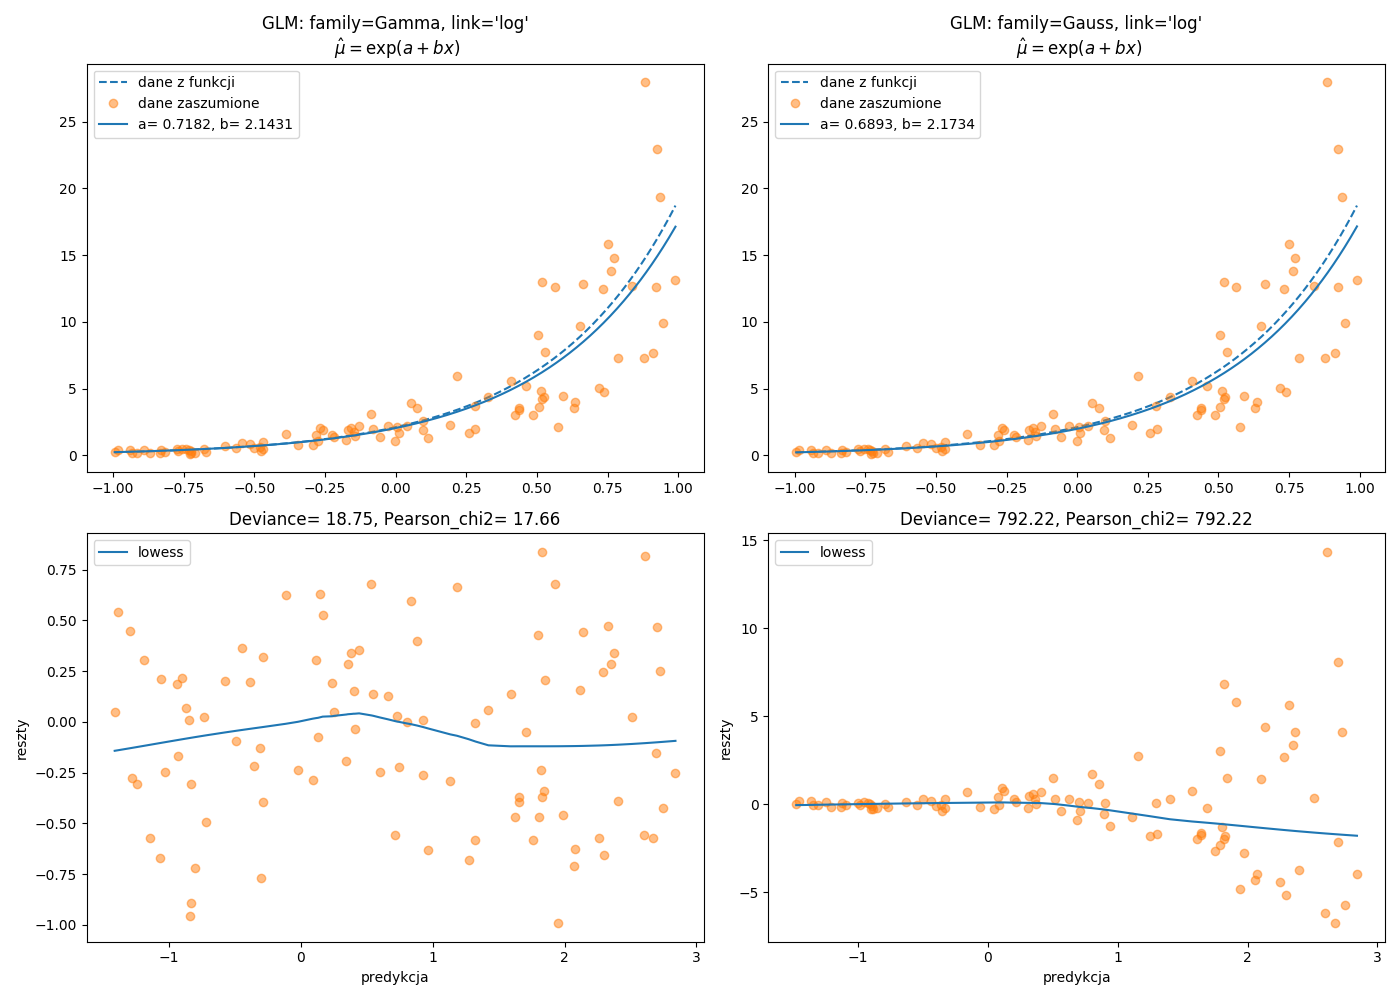
\includegraphics[width=1\linewidth]{modgam01} 

}

\caption{Graficzna prezentacja tej samej funkcji wiążącej z wykorzystaniem dwóch rozkładów.}\label{fig:modgam01}
\end{figure}

\hypertarget{R33}{%
\section{Nieliniowy model gamma regresji}\label{R33}}

Zastosowanie nieliniowego modelu gamma regresji zostanie zaprezentowane na przykładzie zestawu danych \href{https://rdrr.io/rforge/betareg/man/FoodExpenditure.html}{\texttt{FoodExpenditure}}. Są w nim zawarte informacje na temat przychodów i wydatków na żywność z uwzględnieniem liczby osób w gospodarstwie domowym. Wyniki dotyczą próby losowej \(38\) gospodarstw domowych w dużym amerykańskim mieście.

Wykorzystamy parametryzację funkcji \eqref{eq:g05} z parametrami shape oraz scale.
Parametry startowe dla modelu potęgowego oraz Tornquista 1 wyznaczymy odpowiednio na podstawie wzorów \eqref{eq:n08} oraz \eqref{eq:n09}.

\begin{Shaded}
\begin{Highlighting}[]
\ImportTok{import}\NormalTok{ numpy }\ImportTok{as}\NormalTok{ np}
\ImportTok{import}\NormalTok{ scipy.stats }\ImportTok{as}\NormalTok{ stats}
\ImportTok{import}\NormalTok{ matplotlib.pyplot }\ImportTok{as}\NormalTok{ plt}
\ImportTok{import}\NormalTok{ pandas }\ImportTok{as}\NormalTok{ pd}
\ImportTok{import}\NormalTok{ statsmodels.api }\ImportTok{as}\NormalTok{ sm}
\ImportTok{import}\NormalTok{ patsy}
\ImportTok{from}\NormalTok{ scipy.optimize }\ImportTok{import}\NormalTok{ minimize}

\NormalTok{df }\OperatorTok{=}\NormalTok{ pd.read_csv(}\StringTok{"https://raw.githubusercontent.com/krzysiektr/datacsv/master/FoodExpenditure.csv"}\NormalTok{)}

\NormalTok{ly, lx }\OperatorTok{=}\NormalTok{ patsy.dmatrices(}\StringTok{'np.log(food) ~ np.log(income)'}\NormalTok{, df, return_type}\OperatorTok{=}\StringTok{'dataframe'}\NormalTok{)}
\NormalTok{m1 }\OperatorTok{=}\NormalTok{ sm.OLS(ly,lx).fit()}
\NormalTok{p1 }\OperatorTok{=}\NormalTok{ m1.params.values}
\NormalTok{iy, ix }\OperatorTok{=}\NormalTok{ patsy.dmatrices(}\StringTok{'food ~ income'}\NormalTok{, }\DecValTok{1}\OperatorTok{/}\NormalTok{df, return_type}\OperatorTok{=}\StringTok{'dataframe'}\NormalTok{)}
\NormalTok{m2 }\OperatorTok{=}\NormalTok{ sm.OLS(iy,ix).fit()}
\NormalTok{p2 }\OperatorTok{=}\NormalTok{ m2.params.values}

\KeywordTok{def}\NormalTok{ L_gamma_power(par):}
\NormalTok{    mod }\OperatorTok{=}\NormalTok{ par[}\DecValTok{0}\NormalTok{]}\OperatorTok{*}\NormalTok{df[}\StringTok{"income"}\NormalTok{]}\OperatorTok{**}\NormalTok{par[}\DecValTok{1}\NormalTok{]}
\NormalTok{    mu }\OperatorTok{=}\NormalTok{ mod}
\NormalTok{    shape }\OperatorTok{=}\NormalTok{ par[}\DecValTok{2}\NormalTok{]}
\NormalTok{    scale }\OperatorTok{=}\NormalTok{ mu}\OperatorTok{/}\NormalTok{shape}
\NormalTok{    logLik }\OperatorTok{=} \OperatorTok{-}\NormalTok{np.}\BuiltInTok{sum}\NormalTok{( stats.gamma.logpdf(df[}\StringTok{"food"}\NormalTok{], a}\OperatorTok{=}\NormalTok{shape, scale}\OperatorTok{=}\NormalTok{scale) )}
    \ControlFlowTok{return}\NormalTok{(logLik)}

\KeywordTok{def}\NormalTok{ L_gamma_torn1(par):}
\NormalTok{    mod }\OperatorTok{=}\NormalTok{ (par[}\DecValTok{0}\NormalTok{]}\OperatorTok{*}\NormalTok{df[}\StringTok{"income"}\NormalTok{])}\OperatorTok{/}\NormalTok{(df[}\StringTok{"income"}\NormalTok{]}\OperatorTok{+}\NormalTok{par[}\DecValTok{1}\NormalTok{])}
\NormalTok{    mu }\OperatorTok{=}\NormalTok{ mod}
\NormalTok{    shape }\OperatorTok{=}\NormalTok{ par[}\DecValTok{2}\NormalTok{]}
\NormalTok{    scale }\OperatorTok{=}\NormalTok{ mu}\OperatorTok{/}\NormalTok{shape}
\NormalTok{    logLik }\OperatorTok{=} \OperatorTok{-}\NormalTok{np.}\BuiltInTok{sum}\NormalTok{( stats.gamma.logpdf(df[}\StringTok{"food"}\NormalTok{], a}\OperatorTok{=}\NormalTok{shape, scale}\OperatorTok{=}\NormalTok{scale) )}
    \ControlFlowTok{return}\NormalTok{(logLik)}

\NormalTok{initPower }\OperatorTok{=}\NormalTok{ [p1[}\DecValTok{0}\NormalTok{],p1[}\DecValTok{1}\NormalTok{],}\DecValTok{1}\NormalTok{]}
\NormalTok{initTorn1 }\OperatorTok{=}\NormalTok{ [}\DecValTok{1}\OperatorTok{/}\NormalTok{p2[}\DecValTok{0}\NormalTok{],p2[}\DecValTok{1}\NormalTok{]}\OperatorTok{/}\NormalTok{p2[}\DecValTok{0}\NormalTok{],}\DecValTok{1}\NormalTok{]}
\NormalTok{res }\OperatorTok{=}\NormalTok{ minimize(L_gamma_power, initPower, method}\OperatorTok{=} \StringTok{"Nelder-Mead"}\NormalTok{)}
\NormalTok{sol }\OperatorTok{=}\NormalTok{ minimize(L_gamma_torn1, initTorn1, method}\OperatorTok{=} \StringTok{"Nelder-Mead"}\NormalTok{)}

\NormalTok{fig }\OperatorTok{=}\NormalTok{ plt.figure(figsize}\OperatorTok{=}\NormalTok{(}\DecValTok{14}\NormalTok{,}\DecValTok{6}\NormalTok{))}
\NormalTok{ax1 }\OperatorTok{=}\NormalTok{ fig.add_subplot(}\DecValTok{1}\NormalTok{,}\DecValTok{2}\NormalTok{,}\DecValTok{1}\NormalTok{)}
\NormalTok{ax2 }\OperatorTok{=}\NormalTok{ fig.add_subplot(}\DecValTok{1}\NormalTok{,}\DecValTok{2}\NormalTok{,}\DecValTok{2}\NormalTok{)}
\NormalTok{Xg }\OperatorTok{=}\NormalTok{ np.linspace(np.}\BuiltInTok{min}\NormalTok{(df[}\StringTok{"income"}\NormalTok{]),np.}\BuiltInTok{max}\NormalTok{(df[}\StringTok{"income"}\NormalTok{]), }\DecValTok{500}\NormalTok{)}
\NormalTok{ax1.plot(df[}\StringTok{"income"}\NormalTok{],df[}\StringTok{"food"}\NormalTok{],}\StringTok{'o'}\NormalTok{,alpha}\OperatorTok{=}\FloatTok{0.5}\NormalTok{,color}\OperatorTok{=}\StringTok{'C1'}\NormalTok{)}
\NormalTok{ax1.plot(Xg,res.x[}\DecValTok{0}\NormalTok{]}\OperatorTok{*}\NormalTok{Xg}\OperatorTok{**}\NormalTok{res.x[}\DecValTok{1}\NormalTok{],color}\OperatorTok{=}\StringTok{'C0'}\NormalTok{,}
\NormalTok{         label}\OperatorTok{=}\StringTok{'a= }\SpecialCharTok{%.4f}\StringTok{, b= }\SpecialCharTok\NormalTok{ (res.x[}\DecValTok{0}\NormalTok{],res.x[}\DecValTok{1}\NormalTok{]))}
\NormalTok{ax1.set_xlabel(}\StringTok{"income"}\NormalTok{)}
\NormalTok{ax1.set_ylabel(}\StringTok{"food"}\NormalTok{)}
\NormalTok{ax1.set_title(}\StringTok{"Model potęgowy: $y=ax^b$}\CharTok{\textbackslash{}n}\StringTok{ logLik= }\SpecialCharTok{%.4f}\StringTok{, shape= }\SpecialCharTok\NormalTok{ (}\OperatorTok{-}\DecValTok{1}\OperatorTok{*}\NormalTok{res.fun,res.x[}\DecValTok{2}\NormalTok{]))}
\NormalTok{ax1.legend()}
\NormalTok{ax2.plot(df[}\StringTok{"income"}\NormalTok{],df[}\StringTok{"food"}\NormalTok{],}\StringTok{'o'}\NormalTok{,alpha}\OperatorTok{=}\FloatTok{0.5}\NormalTok{,color}\OperatorTok{=}\StringTok{'C1'}\NormalTok{)}
\NormalTok{ax2.plot(Xg,(sol.x[}\DecValTok{0}\NormalTok{]}\OperatorTok{*}\NormalTok{Xg)}\OperatorTok{/}\NormalTok{(Xg}\OperatorTok{+}\NormalTok{sol.x[}\DecValTok{1}\NormalTok{]),color}\OperatorTok{=}\StringTok{'C0'}\NormalTok{,}
\NormalTok{         label}\OperatorTok{=}\StringTok{'a= }\SpecialCharTok{%.4f}\StringTok{, b= }\SpecialCharTok\NormalTok{ (sol.x[}\DecValTok{0}\NormalTok{],sol.x[}\DecValTok{1}\NormalTok{]))}
\NormalTok{ax2.set_xlabel(}\StringTok{"income"}\NormalTok{)}
\NormalTok{ax2.set_ylabel(}\StringTok{"food"}\NormalTok{)}
\NormalTok{ax2.set_title(}\StringTok{"Model Tornquista 1: $y=}\CharTok{\textbackslash{}\textbackslash{}}\StringTok{frac}\SpecialCharTok{\{ax\}}\StringTok{\{x+b\}$}\CharTok{\textbackslash{}n}\StringTok{ logLik= }\SpecialCharTok{%.4f}\StringTok{, shape= }\SpecialCharTok\NormalTok{ (}\OperatorTok{-}\DecValTok{1}\OperatorTok{*}\NormalTok{sol.fun,sol.x[}\DecValTok{2}\NormalTok{]))}
\NormalTok{ax2.legend()}
\NormalTok{fig.tight_layout()}
\NormalTok{plt.savefig(}\StringTok{'nlsGamma01.png'}\NormalTok{)}
\end{Highlighting}
\end{Shaded}

\begin{figure}[h]

{\centering 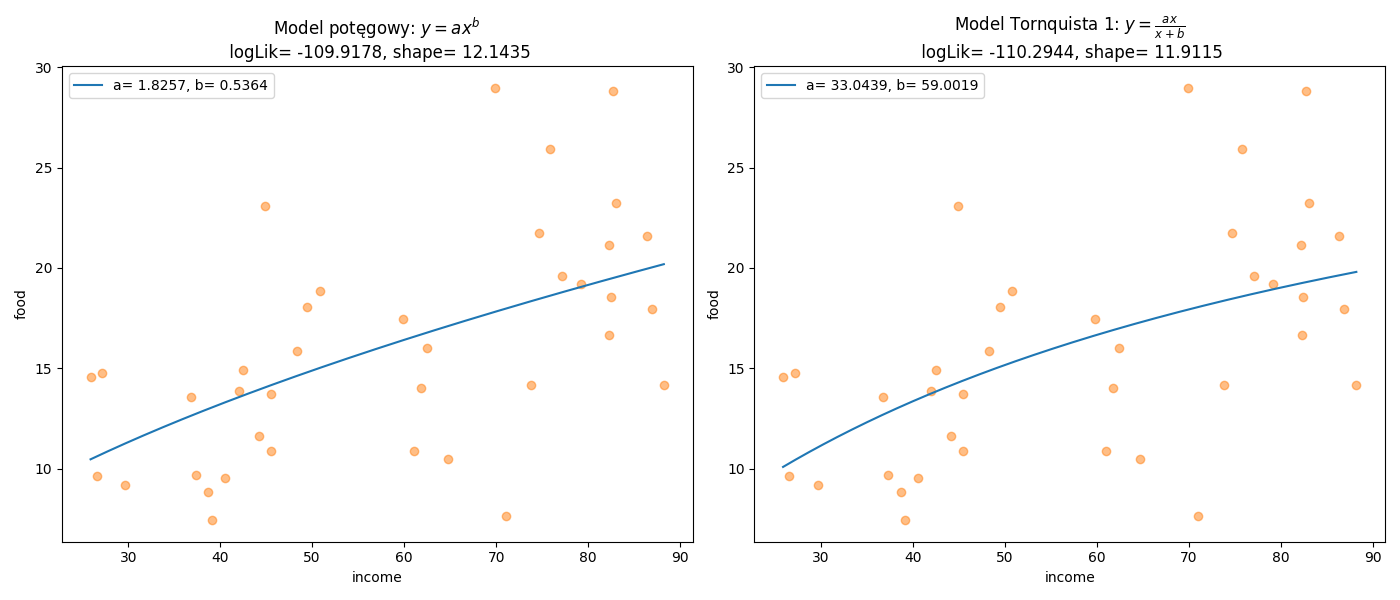
\includegraphics[width=1\linewidth]{nlsGamma01} 

}

\caption{Graficzna prezentacja nieliniowej zależności wydatków na żywność i dochodów.}\label{fig:nlsGamma01}
\end{figure}

\hypertarget{R4}{%
\chapter{Rozkład beta}\label{R4}}

\begin{center}\rule{0.5\linewidth}{\linethickness}\end{center}

\hypertarget{R41}{%
\section{Funkcja gęstości}\label{R41}}

Rozkład beta na przedziale \([a,b]\) został zaimplementowany do funkcji \href{https://docs.scipy.org/doc/scipy-1.2.1/reference/generated/scipy.stats.beta.html\#scipy.stats.beta}{\texttt{scipy.stats.beta}} gdzie: \texttt{loc}\(=a\) oraz \texttt{scale}\(=b-a\). Funkcję gęstości prawdopodobieństwa tego rozkładu można zapisać za pomocą wzoru:
\begin{equation}
f(x\;|\;a,b,\alpha,\beta)=\frac{1}{\mathrm{B}(\alpha,\beta)(b-a)^{\alpha+\beta-1}}(x-a)^{\alpha-1}(b-x)^{\beta-1}
\label{eq:bet01}
\end{equation}
po podstawieniu:
\[\mathrm{B}(\alpha,\beta)(b-a)^{\alpha+\beta-1}=\int_{a}^{b}u^{\alpha-1}(1-u)^{\beta-1}du=\frac{\Gamma(\alpha)\Gamma(\beta)}{\Gamma(\alpha+\beta)}(b-a)^{\alpha+\beta-1}\]
otrzymamy:
\begin{equation}
f(x\;|\;a,b,\alpha,\beta)=\frac{\Gamma(\alpha+\beta)}{\Gamma(\alpha)\Gamma(\beta)(b-a)^{\alpha+\beta-1}}(x-a)^{\alpha-1}(b-x)^{\beta-1}
\label{eq:bet02}
\end{equation}
gdzie: \(E(x)=a+\frac{\alpha}{\alpha+\beta}(b-a)\) oraz \(V(x)=\frac{\alpha\beta}{(\alpha+\beta)^2(\alpha+\beta+1)}(b-a)^2\).

Standardowa wersja rozkładu beta jest rozpatrywana na przedziale \([0;1]\) a więc wzór \eqref{eq:bet02} upraszcza się do postaci:
\begin{equation}
f(x\;|\;\alpha,\beta)=\frac{\Gamma(\alpha+\beta)}{\Gamma(\alpha)\Gamma(\beta)}x^{\alpha-1}(1-x)^{\beta-1}
\label{eq:bet03}
\end{equation}
gdzie: \(E(x)=\frac{\alpha}{\alpha+\beta}\) oraz \(V(x)=\frac{\alpha\beta}{(\alpha+\beta)^2(\alpha+\beta+1)}\).

Jeśli do wzoru \eqref{eq:bet03} podstawimy \(\alpha=\mu\phi\) oraz \(\beta=(1-\mu)\phi\) dla \(\alpha+\beta=\phi\) to otrzymamy:
\begin{equation}
f(x\;|\;\mu,\phi)=\frac{\Gamma(\phi)}{\Gamma(\mu\phi)\Gamma\big((1-\mu)\phi\big)}x^{\mu\phi-1}(1-x)^{(1-\mu)\phi-1}
\label{eq:bet04}
\end{equation}
gdzie: \(E(X)=\mu\) oraz \(V(X)=\frac{\mu(1-\mu)}{1+\phi}\).

Po zlogarytmowaniu funkcji prawdopodobieństwa \eqref{eq:bet04}
otrzymamy funkcję logarytmu wiarygodności o postaci:
\begin{equation}
LL_{beta}=\ln\Gamma(\phi)-\ln\Gamma(\mu\phi)-\ln\Gamma\big((1-\mu)\phi\big)+(\mu\phi-1)\ln(x)+\big((1-\mu)\phi-1\big)\ln(1-x)
\label{eq:betLL01}
\end{equation}

\begin{Shaded}
\begin{Highlighting}[]
\ImportTok{import}\NormalTok{ scipy.stats }\ImportTok{as}\NormalTok{ stats}
  
\NormalTok{y }\OperatorTok{=}\NormalTok{ stats.beta.rvs(}\FloatTok{1.78}\NormalTok{, }\FloatTok{2.34}\NormalTok{, size}\OperatorTok{=}\DecValTok{100}\NormalTok{, random_state}\OperatorTok{=}\DecValTok{2305}\NormalTok{)}

\NormalTok{f }\OperatorTok{=}\NormalTok{ stats.beta.fit(y)}
\NormalTok{logLik }\OperatorTok{=} \BuiltInTok{sum}\NormalTok{(stats.beta.logpdf(y, a}\OperatorTok{=}\NormalTok{f[}\DecValTok{0}\NormalTok{], b}\OperatorTok{=}\NormalTok{f[}\DecValTok{1}\NormalTok{], loc}\OperatorTok{=}\NormalTok{f[}\DecValTok{2}\NormalTok{], scale}\OperatorTok{=}\NormalTok{f[}\DecValTok{3}\NormalTok{]))}

\BuiltInTok{print}\NormalTok{(}\StringTok{"alpha= }\SpecialCharTok{%.4f}\StringTok{, beta= }\SpecialCharTok{%.4f}\StringTok{, loc= }\SpecialCharTok{%.4f}\StringTok{, scale= }\SpecialCharTok\NormalTok{ (f[}\DecValTok{0}\NormalTok{],f[}\DecValTok{1}\NormalTok{],f[}\DecValTok{2}\NormalTok{],f[}\DecValTok{3}\NormalTok{]))}
\BuiltInTok{print}\NormalTok{(}\StringTok{"}\CharTok{\textbackslash{}n}\StringTok{logLik= }\SpecialCharTok\NormalTok{ (logLik))}
\end{Highlighting}
\end{Shaded}

\begin{verbatim}
## alpha= 0.9859, beta= 0.9528, loc= 0.0152, scale= 0.8953
## 
## logLik= 12.6281
\end{verbatim}

\hypertarget{R42}{%
\section{Liniowy model beta regresji}\label{R42}}

Rozkład beta zdefiniowany za pomocą wzoru \eqref{eq:bet04} jest wykorzystywany do budowy liniowego modelu regresji dla proporcji. Inaczej mówiąc, w regresji beta wartości zmiennej zależnej mogą określać np. pewną frakcję dochodów gospodarstw domowych wydawanych na żywność.
Po podstawieniu do wzoru \eqref{eq:betLL01}
\(\hat{\mu}=\frac{1}{1+\exp(-\hat{y})}\) gdzie \(\hat{y}=\beta_0+\sum_{j=1}^{n}\beta_j x_{ij}\) otrzymamy parametry modelu beta regresji. Dodatkowo parametr precyzji \(\phi\) może być uważany za stały lub
można go rozszerzyć o dodatkowy zestaw regresorów tzn. \(\phi=\exp(\hat{y})\).
Zastosowanie liniowego modelu beta regresji zostanie zaprezentowane na przykładzie zestawu danych \href{https://rdrr.io/rforge/betareg/man/FoodExpenditure.html}{\texttt{FoodExpenditure}}.

\begin{Shaded}
\begin{Highlighting}[]
\ImportTok{import}\NormalTok{ numpy }\ImportTok{as}\NormalTok{ np}
\ImportTok{import}\NormalTok{ scipy.stats }\ImportTok{as}\NormalTok{ stats}
\ImportTok{import}\NormalTok{ matplotlib.pyplot }\ImportTok{as}\NormalTok{ plt}
\ImportTok{import}\NormalTok{ pandas }\ImportTok{as}\NormalTok{ pd}
\ImportTok{import}\NormalTok{ statsmodels.api }\ImportTok{as}\NormalTok{ sm}
\ImportTok{import}\NormalTok{ patsy}
\ImportTok{from}\NormalTok{ scipy.optimize }\ImportTok{import}\NormalTok{ minimize}

\NormalTok{df }\OperatorTok{=}\NormalTok{ pd.read_csv(}\StringTok{"https://raw.githubusercontent.com/krzysiektr/datacsv/master/FoodExpenditure.csv"}\NormalTok{)}
\NormalTok{df[}\StringTok{"frac"}\NormalTok{] }\OperatorTok{=}\NormalTok{ df[}\StringTok{"food"}\NormalTok{]}\OperatorTok{/}\NormalTok{df[}\StringTok{"income"}\NormalTok{]}

\NormalTok{y, x }\OperatorTok{=}\NormalTok{ patsy.dmatrices(}\StringTok{'frac ~ income'}\NormalTok{, df, return_type}\OperatorTok{=}\StringTok{'dataframe'}\NormalTok{)}
\NormalTok{ols }\OperatorTok{=}\NormalTok{ sm.OLS(y,x).fit()}
\NormalTok{b }\OperatorTok{=}\NormalTok{ ols.params.values}

\KeywordTok{def}\NormalTok{ L_beta(par):}
\NormalTok{    mod }\OperatorTok{=}\NormalTok{ par[}\DecValTok{0}\NormalTok{]}\OperatorTok{+}\NormalTok{ par[}\DecValTok{1}\NormalTok{]}\OperatorTok{*}\NormalTok{df[}\StringTok{"income"}\NormalTok{]}
\NormalTok{    mu }\OperatorTok{=}\NormalTok{ stats.logistic.cdf(mod)}
\NormalTok{    phi }\OperatorTok{=}\NormalTok{ par[}\DecValTok{2}\NormalTok{]}
\NormalTok{    shape1 }\OperatorTok{=}\NormalTok{ mu}\OperatorTok{*}\NormalTok{phi}
\NormalTok{    shape2 }\OperatorTok{=}\NormalTok{ (}\DecValTok{1}\OperatorTok{-}\NormalTok{mu)}\OperatorTok{*}\NormalTok{phi}
\NormalTok{    logLik }\OperatorTok{=} \OperatorTok{-}\NormalTok{np.}\BuiltInTok{sum}\NormalTok{( stats.beta.logpdf(df[}\StringTok{"frac"}\NormalTok{], a}\OperatorTok{=}\NormalTok{shape1, b}\OperatorTok{=}\NormalTok{shape2) )}
    \ControlFlowTok{return}\NormalTok{(logLik)}

\KeywordTok{def}\NormalTok{ L_gamma(par):}
\NormalTok{    mod }\OperatorTok{=}\NormalTok{ par[}\DecValTok{0}\NormalTok{]}\OperatorTok{+}\NormalTok{ par[}\DecValTok{1}\NormalTok{]}\OperatorTok{*}\NormalTok{df[}\StringTok{"income"}\NormalTok{]}
\NormalTok{    mu }\OperatorTok{=} \DecValTok{1}\OperatorTok{/}\NormalTok{mod}
\NormalTok{    shape }\OperatorTok{=}\NormalTok{ par[}\DecValTok{2}\NormalTok{]}
\NormalTok{    scale }\OperatorTok{=}\NormalTok{ mu}\OperatorTok{/}\NormalTok{shape}
\NormalTok{    logLik }\OperatorTok{=} \OperatorTok{-}\NormalTok{np.}\BuiltInTok{sum}\NormalTok{( stats.gamma.logpdf(df[}\StringTok{"frac"}\NormalTok{], a}\OperatorTok{=}\NormalTok{shape, scale}\OperatorTok{=}\NormalTok{scale) )}
    \ControlFlowTok{return}\NormalTok{(logLik)}

\NormalTok{initParams }\OperatorTok{=}\NormalTok{ [b[}\DecValTok{0}\NormalTok{],b[}\DecValTok{1}\NormalTok{],}\DecValTok{1}\NormalTok{]}
\NormalTok{res }\OperatorTok{=}\NormalTok{ [minimize(i, initParams, method}\OperatorTok{=} \StringTok{"Nelder-Mead"}\NormalTok{) }\ControlFlowTok{for}\NormalTok{ i }\KeywordTok{in}\NormalTok{ [L_beta,L_gamma]]}

\NormalTok{fig }\OperatorTok{=}\NormalTok{ plt.figure(figsize}\OperatorTok{=}\NormalTok{(}\DecValTok{14}\NormalTok{,}\DecValTok{6}\NormalTok{))}
\NormalTok{ax1 }\OperatorTok{=}\NormalTok{ fig.add_subplot(}\DecValTok{1}\NormalTok{,}\DecValTok{2}\NormalTok{,}\DecValTok{1}\NormalTok{)}
\NormalTok{ax2 }\OperatorTok{=}\NormalTok{ fig.add_subplot(}\DecValTok{1}\NormalTok{,}\DecValTok{2}\NormalTok{,}\DecValTok{2}\NormalTok{)}
\NormalTok{Xg }\OperatorTok{=}\NormalTok{ np.linspace(}\DecValTok{20}\NormalTok{,}\DecValTok{150}\NormalTok{, }\DecValTok{1000}\NormalTok{)}
\NormalTok{ax1.plot(df[}\StringTok{"income"}\NormalTok{],df[}\StringTok{"frac"}\NormalTok{],}\StringTok{'o'}\NormalTok{,alpha}\OperatorTok{=}\FloatTok{0.5}\NormalTok{,color}\OperatorTok{=}\StringTok{'C1'}\NormalTok{)}
\NormalTok{ax1.plot(Xg,}\DecValTok{1}\OperatorTok{/}\NormalTok{(}\DecValTok{1}\OperatorTok{+}\NormalTok{np.exp(}\OperatorTok{-}\DecValTok{1}\OperatorTok{*}\NormalTok{(res[}\DecValTok{0}\NormalTok{].x[}\DecValTok{0}\NormalTok{]}\OperatorTok{+}\NormalTok{res[}\DecValTok{0}\NormalTok{].x[}\DecValTok{1}\NormalTok{]}\OperatorTok{*}\NormalTok{Xg))),color}\OperatorTok{=}\StringTok{'C0'}\NormalTok{,}
\NormalTok{         label}\OperatorTok{=}\StringTok{'a= }\SpecialCharTok{%.4f}\StringTok{, b= }\SpecialCharTok\NormalTok{ (res[}\DecValTok{0}\NormalTok{].x[}\DecValTok{0}\NormalTok{],res[}\DecValTok{0}\NormalTok{].x[}\DecValTok{1}\NormalTok{]))}
\NormalTok{ax1.set_xlabel(}\StringTok{"income"}\NormalTok{)}
\NormalTok{ax1.set_ylabel(}\StringTok{"frac"}\NormalTok{)}
\NormalTok{ax1.set_title(}\StringTok{"GLM: Rozkład beta - model logistyczny: $}\CharTok{\textbackslash{}\textbackslash{}}\StringTok{hat\{}\CharTok{\textbackslash{}\textbackslash{}}\StringTok{mu\}=}\CharTok{\textbackslash{}\textbackslash{}}\StringTok{frac}\SpecialCharTok{\{1\}}\StringTok{\{1+}\CharTok{\textbackslash{}\textbackslash{}}\StringTok{exp(-(a+bx))\}$}\CharTok{\textbackslash{}n}\StringTok{ logLik= }\SpecialCharTok{%.4f}\StringTok{, phi= }\SpecialCharTok\NormalTok{ (}\OperatorTok{-}\DecValTok{1}\OperatorTok{*}\NormalTok{res[}\DecValTok{0}\NormalTok{].fun,res[}\DecValTok{0}\NormalTok{].x[}\DecValTok{2}\NormalTok{]))}
\NormalTok{ax1.legend()}
\NormalTok{ax2.plot(df[}\StringTok{"income"}\NormalTok{],df[}\StringTok{"frac"}\NormalTok{],}\StringTok{'o'}\NormalTok{,alpha}\OperatorTok{=}\FloatTok{0.5}\NormalTok{,color}\OperatorTok{=}\StringTok{'C1'}\NormalTok{)}
\NormalTok{ax2.plot(Xg,}\DecValTok{1}\OperatorTok{/}\NormalTok{(res[}\DecValTok{1}\NormalTok{].x[}\DecValTok{0}\NormalTok{]}\OperatorTok{+}\NormalTok{res[}\DecValTok{1}\NormalTok{].x[}\DecValTok{1}\NormalTok{]}\OperatorTok{*}\NormalTok{Xg),color}\OperatorTok{=}\StringTok{'C0'}\NormalTok{,}
\NormalTok{         label}\OperatorTok{=}\StringTok{'a= }\SpecialCharTok{%.4f}\StringTok{, b= }\SpecialCharTok\NormalTok{ (res[}\DecValTok{1}\NormalTok{].x[}\DecValTok{0}\NormalTok{],res[}\DecValTok{1}\NormalTok{].x[}\DecValTok{1}\NormalTok{]))}
\NormalTok{ax2.set_xlabel(}\StringTok{"income"}\NormalTok{)}
\NormalTok{ax2.set_ylabel(}\StringTok{"frac"}\NormalTok{)}
\NormalTok{ax2.set_title(}\StringTok{"GLM: Rozkład gamma - model odwrotny: $}\CharTok{\textbackslash{}\textbackslash{}}\StringTok{hat\{}\CharTok{\textbackslash{}\textbackslash{}}\StringTok{mu\}=}\CharTok{\textbackslash{}\textbackslash{}}\StringTok{frac}\SpecialCharTok{\{1\}}\StringTok{\{a+bx\}$}\CharTok{\textbackslash{}n}\StringTok{ logLik= }\SpecialCharTok{%.4f}\StringTok{, phi= }\SpecialCharTok\NormalTok{ (}\OperatorTok{-}\DecValTok{1}\OperatorTok{*}\NormalTok{res[}\DecValTok{1}\NormalTok{].fun,res[}\DecValTok{1}\NormalTok{].x[}\DecValTok{2}\NormalTok{]))}
\NormalTok{ax2.legend()}
\NormalTok{fig.tight_layout()}
\NormalTok{plt.savefig(}\StringTok{'prop01.png'}\NormalTok{)}
\end{Highlighting}
\end{Shaded}

\begin{figure}[h]

{\centering 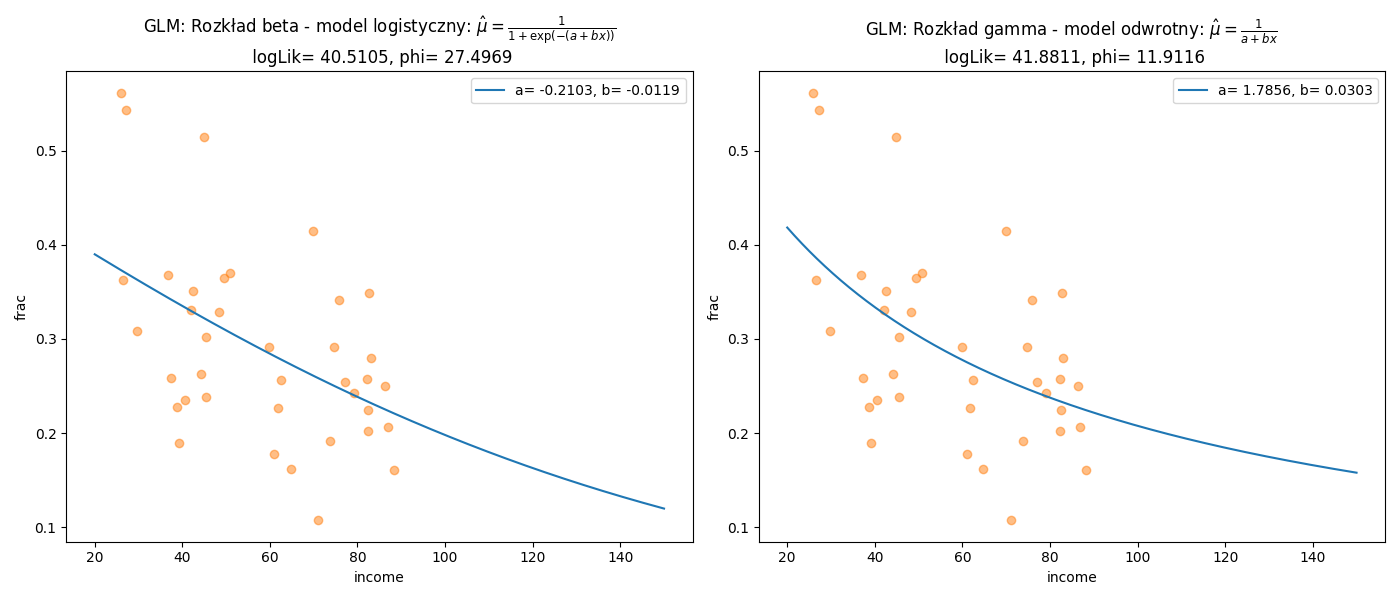
\includegraphics[width=1\linewidth]{prop01} 

}

\caption{Graficzna prezentacja nieliniowej zależności frakcji wydatków na żywność i dochodów.}\label{fig:prop01}
\end{figure}

\hypertarget{R5}{%
\chapter{Rozkład beta dwumianowy}\label{R5}}

\begin{center}\rule{0.5\linewidth}{\linethickness}\end{center}

\hypertarget{R51}{%
\section{Funkcja gęstości}\label{R51}}

Złożenie dwóch rozkładów: dwumianowego oraz beta na przedziale \((0,1)\) tworzy rozkład beta dwumianowy o postaci:
\begin{equation}
f(x\;|\;n,\alpha,\beta)=\displaystyle\underbrace{{n\choose x}\;p^x (1-p)^{n-x}}_{\mbox{rozkład dwumianowy}} \cdot \displaystyle\underbrace{\frac{1}{\mathrm{B}(\alpha,\beta)}p^{\alpha-1}(1-p)^{\beta-1}}_{\mbox{rozkład beta}}
\label{eq:bb01}
\end{equation}
w którym po podstawieniu:
\[{n \choose x}=\frac{\Gamma(n+1)}{\Gamma(x+1)\Gamma(n-x+1)}\quad \mbox{oraz}\quad p^{x+\alpha-1}(1-p)^{n-x+\beta-1}=\mathrm{B}(x+\alpha,\;n-x+\beta)\]
otrzymamy:
\begin{equation}
f(x\;|\;n,\alpha,\beta)=\frac{\Gamma(n+1)}{\Gamma(x+1)\Gamma(n-x+1)}\cdot\frac{1}{\mathrm{B}(\alpha,\beta)}\cdot \mathrm{B}(x+\alpha, \;n-x+\beta)
\label{eq:bb02}
\end{equation}
gdzie:
\(E(X)=n\frac{\alpha}{\alpha+\beta}\) oraz \(V(X)=n\frac{\alpha\beta(\alpha+\beta+n)}{(\alpha+\beta)^2(\alpha+\beta+1)}\).

Za pomocą rozkładu beta dwumianowego \(f(x\;|\;n,\alpha,\beta)\) można przybliżać rozkład dwumianowy
gdzie: \(\alpha=n\) oraz \(\beta=n(1-p)/p\).

\begin{Shaded}
\begin{Highlighting}[]
\ImportTok{import}\NormalTok{ numpy }\ImportTok{as}\NormalTok{ np}
\ImportTok{import}\NormalTok{ scipy.stats }\ImportTok{as}\NormalTok{ stats}
\ImportTok{import}\NormalTok{ scipy.special }\ImportTok{as}\NormalTok{ spec}
\ImportTok{import}\NormalTok{ matplotlib.pyplot }\ImportTok{as}\NormalTok{ plt}

\KeywordTok{def}\NormalTok{ bb(x,n,alpha,beta):}
\NormalTok{    B1 }\OperatorTok{=}\NormalTok{ (spec.gamma(n}\OperatorTok{+}\DecValTok{1}\NormalTok{)}\OperatorTok{*}\NormalTok{spec.beta(x}\OperatorTok{+}\NormalTok{alpha,n}\OperatorTok{-}\NormalTok{x}\OperatorTok{+}\NormalTok{beta))}
\NormalTok{    B2 }\OperatorTok{=}\NormalTok{ (spec.gamma(x}\OperatorTok{+}\DecValTok{1}\NormalTok{)}\OperatorTok{*}\NormalTok{spec.gamma(n}\OperatorTok{-}\NormalTok{x}\OperatorTok{+}\DecValTok{1}\NormalTok{)}\OperatorTok{*}\NormalTok{spec.beta(alpha,beta))}
    \ControlFlowTok{return}\NormalTok{(B1}\OperatorTok{/}\NormalTok{B2)}

\NormalTok{x }\OperatorTok{=}\NormalTok{ [}\DecValTok{0}\NormalTok{,}\DecValTok{1}\NormalTok{,}\DecValTok{2}\NormalTok{,}\DecValTok{3}\NormalTok{,}\DecValTok{4}\NormalTok{,}\DecValTok{5}\NormalTok{,}\DecValTok{6}\NormalTok{,}\DecValTok{7}\NormalTok{,}\DecValTok{8}\NormalTok{,}\DecValTok{9}\NormalTok{,}\DecValTok{10}\NormalTok{]}
\NormalTok{n }\OperatorTok{=} \DecValTok{50}
\NormalTok{p }\OperatorTok{=} \FloatTok{0.1}
\NormalTok{BB }\OperatorTok{=}\NormalTok{ [bb(i,n,n,n}\OperatorTok{*}\NormalTok{(}\DecValTok{1}\OperatorTok{-}\NormalTok{p)}\OperatorTok{/}\NormalTok{p).}\BuiltInTok{round}\NormalTok{(}\DecValTok{7}\NormalTok{) }\ControlFlowTok{for}\NormalTok{ i }\KeywordTok{in}\NormalTok{ x]}
\NormalTok{B  }\OperatorTok{=}\NormalTok{ [stats.binom.pmf(i,n,p).}\BuiltInTok{round}\NormalTok{(}\DecValTok{7}\NormalTok{) }\ControlFlowTok{for}\NormalTok{ i }\KeywordTok{in}\NormalTok{ x]}
\NormalTok{fig }\OperatorTok{=}\NormalTok{ plt.figure(figsize}\OperatorTok{=}\NormalTok{(}\DecValTok{14}\NormalTok{,}\DecValTok{6}\NormalTok{))}
\NormalTok{ax1 }\OperatorTok{=}\NormalTok{ fig.add_subplot(}\DecValTok{1}\NormalTok{,}\DecValTok{2}\NormalTok{,}\DecValTok{1}\NormalTok{)}
\NormalTok{ax2 }\OperatorTok{=}\NormalTok{ fig.add_subplot(}\DecValTok{1}\NormalTok{,}\DecValTok{2}\NormalTok{,}\DecValTok{2}\NormalTok{)}
\NormalTok{ax1.vlines(x, }\DecValTok{0}\NormalTok{, B, colors}\OperatorTok{=}\StringTok{'k'}\NormalTok{, linestyles}\OperatorTok{=}\StringTok{'-'}\NormalTok{, lw}\OperatorTok{=}\DecValTok{10}\NormalTok{,}\OperatorTok{\textbackslash{}}
\NormalTok{           label}\OperatorTok{=}\StringTok{'dwumianowy'}\NormalTok{)   }
\NormalTok{ax1.vlines(x, }\DecValTok{0}\NormalTok{, BB, colors}\OperatorTok{=}\StringTok{'orange'}\NormalTok{, linestyles}\OperatorTok{=}\StringTok{'-'}\NormalTok{, lw}\OperatorTok{=}\DecValTok{3}\NormalTok{,}\OperatorTok{\textbackslash{}}
\NormalTok{           label}\OperatorTok{=}\StringTok{'beta dwumianowy'}\NormalTok{)}
\NormalTok{ax1.set_title(}\StringTok{'Parametry: n=%.0f, p=}\SpecialCharTok{%.1f}\StringTok{, alpha= %.0f, beta=%.0f'} \OperatorTok{%}\NormalTok{ (n,p,n,n}\OperatorTok{*}\NormalTok{(}\DecValTok{1}\OperatorTok{-}\NormalTok{p)}\OperatorTok{/}\NormalTok{p))}
\NormalTok{ax1.set_ylabel(}\StringTok{'prawdopodobieństwo rozkładu'}\NormalTok{)}
\NormalTok{ax1.legend(loc}\OperatorTok{=}\StringTok{'best'}\NormalTok{, frameon}\OperatorTok{=}\VariableTok{False}\NormalTok{) }
\NormalTok{ax2.plot(B,BB,}\StringTok{'o'}\NormalTok{,color}\OperatorTok{=}\StringTok{'k'}\NormalTok{,label}\OperatorTok{=}\StringTok{'zależność empiryczna'}\NormalTok{)}
\NormalTok{ax2.plot([}\DecValTok{0}\NormalTok{,}\BuiltInTok{max}\NormalTok{(B)],[}\DecValTok{0}\NormalTok{,}\BuiltInTok{max}\NormalTok{(B)],color}\OperatorTok{=}\StringTok{'orange'}\NormalTok{,label}\OperatorTok{=}\StringTok{'zależność liniowa'}\NormalTok{)}
\NormalTok{ax2.set_title(}\StringTok{'Parametry: n=%.0f, p=}\SpecialCharTok{%.1f}\StringTok{, alpha= %.0f, beta=%.0f'} \OperatorTok{%}\NormalTok{ (n,p,n,n}\OperatorTok{*}\NormalTok{(}\DecValTok{1}\OperatorTok{-}\NormalTok{p)}\OperatorTok{/}\NormalTok{p))}
\NormalTok{ax2.set_xlabel(}\StringTok{'prawdopodobieństwo rozkładu dwumianowego'}\NormalTok{)}
\NormalTok{ax2.set_ylabel(}\StringTok{'prawdopodobieństwo rozkładu beta dwumianowego'}\NormalTok{)}
\NormalTok{ax2.legend(loc}\OperatorTok{=}\StringTok{'best'}\NormalTok{, frameon}\OperatorTok{=}\VariableTok{False}\NormalTok{)}
\NormalTok{plt.tight_layout()}
\NormalTok{plt.savefig(}\StringTok{"betabinom.png"}\NormalTok{)}
\end{Highlighting}
\end{Shaded}

\begin{figure}[h]

{\centering 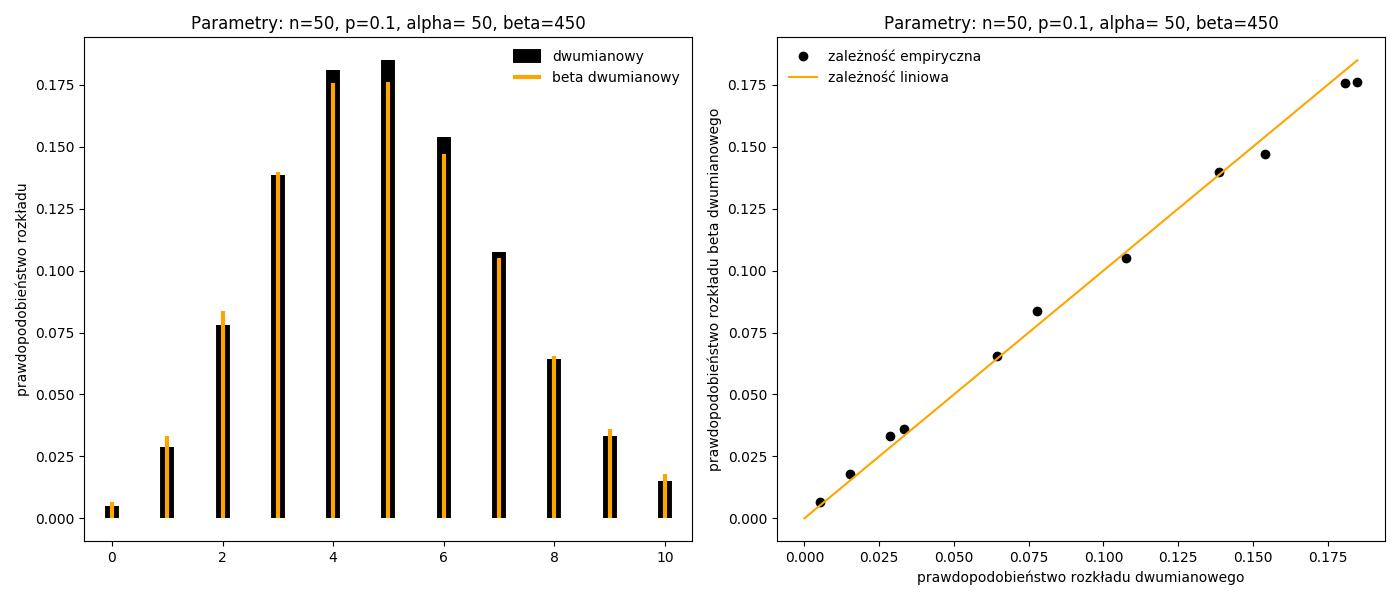
\includegraphics[width=1\linewidth]{betabinom} 

}

\caption{Przybliżanie rozkładu dwumianowego rozkładem beta dwumianowym.}\label{fig:betabinom}
\end{figure}

Po uwzględnieniu parametryzacji:
\(\alpha=\mu\rho^{-1}(1-\rho)\) i \(\beta=(1-\mu)\rho^{-1}(1-\rho)\) lub \(\alpha=\mu/\sigma\) i \(\beta=(1-\mu)/\sigma\)
otrzymamy zmodyfikowany rozkład beta dwumianowy w którym funkcję logarytmu wiarygodności można zapisać za pomocą wzoru:
\begin{equation}
LL=\ln\Gamma(n+1)+\ln \mathrm{B}\left(x+\frac{\mu}{\sigma},n-x+\frac{1-\mu}{\sigma}\right)-\ln\Gamma(x+1)-\ln\Gamma(n-x+1)-\ln \mathrm{B}\left(\frac{\mu}{\sigma},\frac{1-\mu}{\sigma}\right)
\label{eq:bb03}
\end{equation}

\hypertarget{R52}{%
\section{Liniowy model beta dwumianowej regresji}\label{R52}}

Zastosowanie liniowego modelu beta dwumianowej regresji zostanie zaprezentowane na przykładzie zestawu danych \href{https://github.com/mwaskom/seaborn-data/blob/master/titanic.csv}{\texttt{titanic}}. Na ich podstawie
możemy obliczyć prawdopodobieństwo ocalenia życia w katastrofie brytyjskiego transatlantyka Titanic w
zależności od wieku pasażera oraz klasy podróżowania.

\begin{Shaded}
\begin{Highlighting}[]
\ImportTok{import}\NormalTok{ warnings}
\NormalTok{warnings.filterwarnings(}\StringTok{"ignore"}\NormalTok{)}

\ImportTok{import}\NormalTok{ seaborn }\ImportTok{as}\NormalTok{ sns}
\ImportTok{import}\NormalTok{ numpy }\ImportTok{as}\NormalTok{ np}
\ImportTok{import}\NormalTok{ pandas }\ImportTok{as}\NormalTok{ pd}
\ImportTok{import}\NormalTok{ matplotlib.pyplot }\ImportTok{as}\NormalTok{ plt}
  
\NormalTok{df }\OperatorTok{=}\NormalTok{ sns.load_dataset(}\StringTok{"titanic"}\NormalTok{)}

\NormalTok{fig }\OperatorTok{=}\NormalTok{ plt.figure(figsize}\OperatorTok{=}\NormalTok{(}\DecValTok{14}\NormalTok{,}\DecValTok{6}\NormalTok{))}
\NormalTok{ax1 }\OperatorTok{=}\NormalTok{ fig.add_subplot(}\DecValTok{1}\NormalTok{,}\DecValTok{2}\NormalTok{,}\DecValTok{1}\NormalTok{)}
\NormalTok{ax2 }\OperatorTok{=}\NormalTok{ fig.add_subplot(}\DecValTok{1}\NormalTok{,}\DecValTok{2}\NormalTok{,}\DecValTok{2}\NormalTok{)}
\NormalTok{sns.countplot(x }\OperatorTok{=} \StringTok{'survived'}\NormalTok{, data }\OperatorTok{=}\NormalTok{ df, palette }\OperatorTok{=} \StringTok{'YlOrRd'}\NormalTok{,ax}\OperatorTok{=}\NormalTok{ax1)}
\NormalTok{sns.heatmap(df[[}\StringTok{'survived'}\NormalTok{,}\StringTok{'pclass'}\NormalTok{,}\StringTok{'age'}\NormalTok{]].isnull(),cmap}\OperatorTok{=}\StringTok{'YlOrRd'}\NormalTok{,ax}\OperatorTok{=}\NormalTok{ax2)}
\NormalTok{plt.tight_layout()}
\NormalTok{plt.savefig(}\StringTok{"titanic.png"}\NormalTok{)}
\end{Highlighting}
\end{Shaded}

\begin{figure}[h]

{\centering 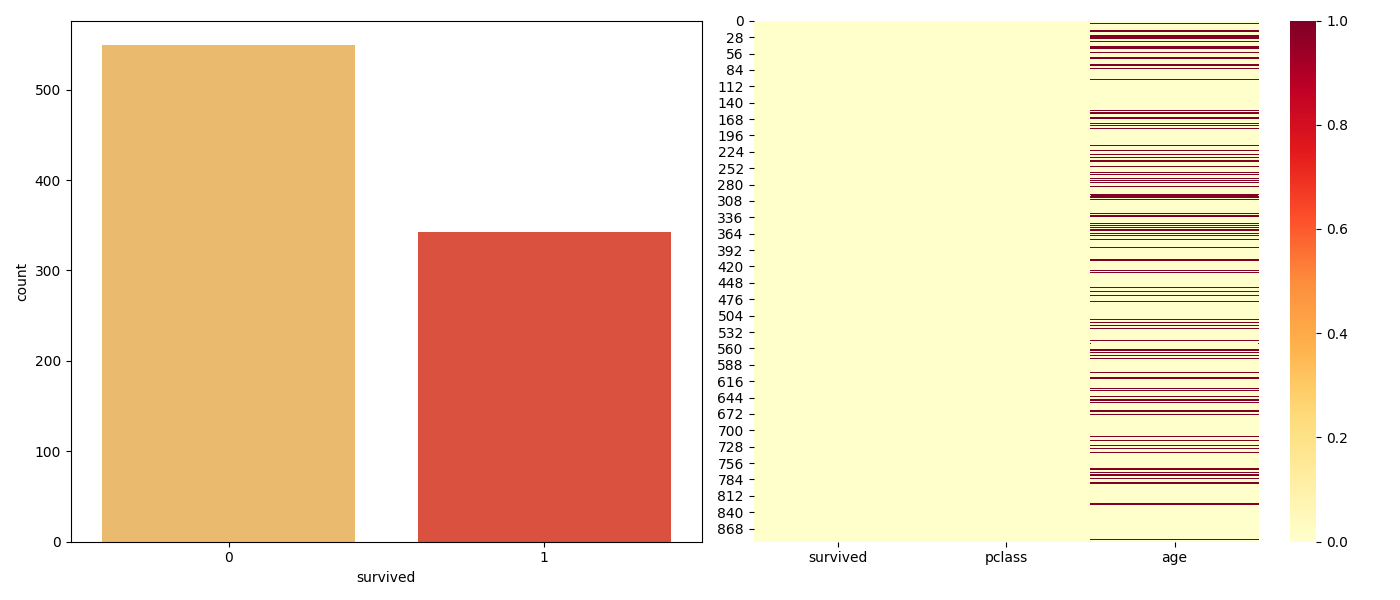
\includegraphics[width=1\linewidth]{titanic} 

}

\caption{Graficzna prezentacja danych Titanic.}\label{fig:titanic}
\end{figure}

Rozkład beta dwumianowy jest wykorzystywany do budowy liniowego modelu regresji dla danych binarnych jako alternatywa np. dla regresji logitowej/probitowej. W tym zastosowaniu optymalizujemy (maksymalizacja) funkcję daną wzorem \eqref{eq:bb03} w której \(\hat{\mu}=\frac{1}{1+\exp(-\hat{y})}\) dla \(\hat{y}=\beta_0+\sum_{j=1}^{n}\beta_j x_{ij}\) otrzymamy parametry modelu beta dwumianowej regresji.

\begin{Shaded}
\begin{Highlighting}[]
\ImportTok{import}\NormalTok{ seaborn }\ImportTok{as}\NormalTok{ sns}
\ImportTok{import}\NormalTok{ numpy }\ImportTok{as}\NormalTok{ np}
\ImportTok{import}\NormalTok{ scipy.stats }\ImportTok{as}\NormalTok{ stats}
\ImportTok{import}\NormalTok{ pandas }\ImportTok{as}\NormalTok{ pd}
\ImportTok{import}\NormalTok{ scipy.special }\ImportTok{as}\NormalTok{ spec}
\ImportTok{from}\NormalTok{ scipy.optimize }\ImportTok{import}\NormalTok{ minimize}
\ImportTok{import}\NormalTok{ patsy}

\NormalTok{df }\OperatorTok{=}\NormalTok{ sns.load_dataset(}\StringTok{"titanic"}\NormalTok{).dropna()}
\NormalTok{survived }\OperatorTok{=}\NormalTok{ df[}\StringTok{'survived'}\NormalTok{]}
\NormalTok{pclass }\OperatorTok{=}\NormalTok{ df[}\StringTok{'pclass'}\NormalTok{]}
\NormalTok{age }\OperatorTok{=}\NormalTok{ df[}\StringTok{'age'}\NormalTok{]}
\NormalTok{yObs, xObs }\OperatorTok{=}\NormalTok{ patsy.dmatrices(}\StringTok{'survived ~ pclass + age'}\NormalTok{, df, return_type}\OperatorTok{=}\StringTok{'dataframe'}\NormalTok{)}
\NormalTok{b0, b1, b2 }\OperatorTok{=}\NormalTok{ np.linalg.lstsq(xObs, yObs, rcond}\OperatorTok{=}\VariableTok{None}\NormalTok{)[}\DecValTok{0}\NormalTok{]}

\KeywordTok{def}\NormalTok{ Lbb(x,mu,sigma,n):}
    \ControlFlowTok{return}\NormalTok{ spec.loggamma(n}\OperatorTok{+}\DecValTok{1}\NormalTok{)}\OperatorTok{+}\NormalTok{spec.betaln(x}\OperatorTok{+}\NormalTok{mu}\OperatorTok{/}\NormalTok{sigma,n}\OperatorTok{-}\NormalTok{x}\OperatorTok{+}\NormalTok{((}\DecValTok{1}\OperatorTok{-}\NormalTok{mu)}\OperatorTok{/}\NormalTok{sigma))}\OperatorTok{-\textbackslash{}}
\NormalTok{           spec.loggamma(x}\OperatorTok{+}\DecValTok{1}\NormalTok{)}\OperatorTok{-}\NormalTok{spec.loggamma(n}\OperatorTok{-}\NormalTok{x}\OperatorTok{+}\DecValTok{1}\NormalTok{)}\OperatorTok{-}\NormalTok{spec.betaln(mu}\OperatorTok{/}\NormalTok{sigma,(}\DecValTok{1}\OperatorTok{-}\NormalTok{mu)}\OperatorTok{/}\NormalTok{sigma)}

\KeywordTok{def}\NormalTok{ h(par):}
\NormalTok{    mod }\OperatorTok{=}\NormalTok{ par[}\DecValTok{0}\NormalTok{] }\OperatorTok{+}\NormalTok{par[}\DecValTok{1}\NormalTok{]}\OperatorTok{*}\NormalTok{pclass }\OperatorTok{+}\NormalTok{par[}\DecValTok{2}\NormalTok{]}\OperatorTok{*}\NormalTok{age}
\NormalTok{    MU  }\OperatorTok{=}\NormalTok{ stats.logistic.cdf(mod)}
\NormalTok{    SIGMA }\OperatorTok{=}\NormalTok{ par[}\DecValTok{3}\NormalTok{]}
\NormalTok{    logLik }\OperatorTok{=} \OperatorTok{-}\NormalTok{np.}\BuiltInTok{sum}\NormalTok{( Lbb(survived, mu}\OperatorTok{=}\NormalTok{MU, sigma}\OperatorTok{=}\NormalTok{SIGMA, n}\OperatorTok{=}\DecValTok{1}\NormalTok{) )}
    \ControlFlowTok{return}\NormalTok{(logLik)}

\NormalTok{initParams }\OperatorTok{=}\NormalTok{ [b0[}\DecValTok{0}\NormalTok{],b1[}\DecValTok{0}\NormalTok{],b2[}\DecValTok{0}\NormalTok{],}\DecValTok{1}\NormalTok{]}
\NormalTok{bnds }\OperatorTok{=}\NormalTok{ ((}\VariableTok{None}\NormalTok{, }\VariableTok{None}\NormalTok{), (}\VariableTok{None}\NormalTok{,}\VariableTok{None}\NormalTok{),(}\VariableTok{None}\NormalTok{, }\VariableTok{None}\NormalTok{), (}\DecValTok{0}\NormalTok{,}\VariableTok{None}\NormalTok{))}
\NormalTok{results }\OperatorTok{=}\NormalTok{ minimize(h, initParams, method}\OperatorTok{=} \StringTok{"L-BFGS-B"}\NormalTok{, bounds}\OperatorTok{=}\NormalTok{bnds)}
\BuiltInTok{print}\NormalTok{(}\StringTok{"GLM: family= beta-binomial, link= logistic}\CharTok{\textbackslash{}n}\StringTok{"}\NormalTok{)}
\BuiltInTok{print}\NormalTok{(}\StringTok{"const= }\SpecialCharTok{%.4f}\StringTok{, pclass= }\SpecialCharTok{%.4f}\StringTok{, age= }\SpecialCharTok{%.4f}\StringTok{, phi= }\SpecialCharTok\NormalTok{ (results.x[}\DecValTok{0}\NormalTok{],results.x[}\DecValTok{1}\NormalTok{],results.x[}\DecValTok{2}\NormalTok{],results.x[}\DecValTok{3}\NormalTok{]))}
\BuiltInTok{print}\NormalTok{(}\StringTok{"}\CharTok{\textbackslash{}n}\StringTok{logLik= }\SpecialCharTok\NormalTok{ (}\OperatorTok{-}\DecValTok{1}\OperatorTok{*}\NormalTok{results.fun))}
\end{Highlighting}
\end{Shaded}

\begin{verbatim}
## GLM: family= beta-binomial, link= logistic
## 
## const= 2.9762, pclass= -0.5559, age= -0.0424, phi= 1.0000
## 
## logLik= -107.3699
\end{verbatim}

Wyniki można porównać ze standardowym rozwiązaniem tzn. liniowym modelem regresji logitowej lub probitowej. W optymalizacji funkcji logarytmu wiarygodności rozkładu dwumianowego wykorzystujemy dystrybuantę rozkładu logistycznego (logit) lub normalnego (probit). Instnieje pewna zależność pomiędzy parametrami z tych dwóch modeli tzn. \(\beta_{probit} \approx 1.6\cdot\beta_{logit}\). Dodatkowo można wyznaczyć efekty krańcowe za pomocą funkcji \href{https://www.statsmodels.org/dev/generated/statsmodels.discrete.discrete_model.CountResults.get_margeff.html}{\texttt{get\_margeff}}. Krzywa ROC informuje nas o jakości modelu tzn. im wykres bardziej ``wypukły'', tym lepszy model. Zatm pole pod krzywą (AUC - Area Under ROC Curve) powinno być większe od \(0.5\).

\begin{Shaded}
\begin{Highlighting}[]
\ImportTok{import}\NormalTok{ pandas }\ImportTok{as}\NormalTok{ pd}
\ImportTok{import}\NormalTok{ statsmodels.api }\ImportTok{as}\NormalTok{ sm}
\ImportTok{import}\NormalTok{ patsy}
\ImportTok{import}\NormalTok{ seaborn }\ImportTok{as}\NormalTok{ sns}
\ImportTok{from}\NormalTok{ sklearn.metrics }\ImportTok{import}\NormalTok{ roc_curve, auc, confusion_matrix}
\ImportTok{import}\NormalTok{ numpy }\ImportTok{as}\NormalTok{ np}
\ImportTok{import}\NormalTok{ matplotlib.pyplot }\ImportTok{as}\NormalTok{ plt}

\NormalTok{df }\OperatorTok{=}\NormalTok{ sns.load_dataset(}\StringTok{"titanic"}\NormalTok{).dropna()}
\NormalTok{y, x }\OperatorTok{=}\NormalTok{ patsy.dmatrices(}\StringTok{'survived ~ pclass + age'}\NormalTok{, df, return_type}\OperatorTok{=}\StringTok{'dataframe'}\NormalTok{)}
      
\NormalTok{logit }\OperatorTok{=}\NormalTok{ sm.Logit(y,x).fit()}
\BuiltInTok{print}\NormalTok{(logit.params)}

\NormalTok{yp }\OperatorTok{=}\NormalTok{ logit.predict()}
\NormalTok{fpr, tpr, thresholds }\OperatorTok{=}\NormalTok{ roc_curve(y, yp)}
\NormalTok{aur }\OperatorTok{=}\NormalTok{ auc(fpr,tpr)}
\NormalTok{sens }\OperatorTok{=}\NormalTok{ tpr[thresholds }\OperatorTok{>} \FloatTok{0.5}\NormalTok{][}\OperatorTok{-}\DecValTok{1}\NormalTok{]     }\CommentTok{# czułość}
\NormalTok{spec }\OperatorTok{=} \DecValTok{1} \OperatorTok{-}\NormalTok{ fpr[thresholds }\OperatorTok{>} \FloatTok{0.5}\NormalTok{][}\OperatorTok{-}\DecValTok{1}\NormalTok{] }\CommentTok{# specyficzność}
\NormalTok{xx }\OperatorTok{=}\NormalTok{ np.arange(}\DecValTok{101}\NormalTok{) }\OperatorTok{/} \BuiltInTok{float}\NormalTok{(}\DecValTok{100}\NormalTok{)}
\NormalTok{ypp }\OperatorTok{=}\NormalTok{ (yp}\OperatorTok{>}\FloatTok{0.5}\NormalTok{).astype(}\BuiltInTok{int}\NormalTok{)}
\NormalTok{tab }\OperatorTok{=}\NormalTok{ confusion_matrix(y,ypp)}
\NormalTok{tn, fp, fn, tp }\OperatorTok{=}\NormalTok{ confusion_matrix(y,ypp).ravel()}

\NormalTok{fig }\OperatorTok{=}\NormalTok{ plt.figure(figsize}\OperatorTok{=}\NormalTok{(}\DecValTok{14}\NormalTok{,}\DecValTok{6}\NormalTok{))}
\NormalTok{ax1 }\OperatorTok{=}\NormalTok{ fig.add_subplot(}\DecValTok{1}\NormalTok{,}\DecValTok{2}\NormalTok{,}\DecValTok{1}\NormalTok{)}
\NormalTok{ax2 }\OperatorTok{=}\NormalTok{ fig.add_subplot(}\DecValTok{1}\NormalTok{,}\DecValTok{2}\NormalTok{,}\DecValTok{2}\NormalTok{)}
\NormalTok{ax1.plot([}\DecValTok{0}\NormalTok{,}\DecValTok{0}\NormalTok{,}\DecValTok{1}\NormalTok{],[}\DecValTok{0}\NormalTok{,}\DecValTok{1}\NormalTok{,}\DecValTok{1}\NormalTok{], }\StringTok{'--'}\NormalTok{, color}\OperatorTok{=}\StringTok{'k'}\NormalTok{, label}\OperatorTok{=}\StringTok{'AUC = 1'}\NormalTok{)}
\NormalTok{ax1.plot(fpr,tpr, color}\OperatorTok{=}\StringTok{'orange'}\NormalTok{)}
\NormalTok{ax1.plot(xx,xx, }\StringTok{':'}\NormalTok{, color}\OperatorTok{=}\StringTok{'k'}\NormalTok{, label}\OperatorTok{=}\StringTok{'AUC = 0.5'}\NormalTok{)}
\NormalTok{ax1.fill_between(x}\OperatorTok{=}\NormalTok{fpr, y1}\OperatorTok{=}\NormalTok{tpr, color}\OperatorTok{=}\StringTok{'orange'}\NormalTok{, alpha}\OperatorTok{=}\FloatTok{0.35}\NormalTok{, label}\OperatorTok{=}\StringTok{'AUC = }\SpecialCharTok\NormalTok{ aur)}
\NormalTok{ax1.set_title(}\StringTok{"Krzywa ROC oraz wartość AUC"}\NormalTok{)}
\NormalTok{ax1.set_xlabel(}\StringTok{'specyficzność - specificity'}\NormalTok{)}
\NormalTok{ax1.set_ylabel(}\StringTok{'czułość - sensitivity'}\NormalTok{)}
\NormalTok{ax1.legend()}
\NormalTok{sns.heatmap(tab,annot}\OperatorTok{=}\VariableTok{True}\NormalTok{, fmt}\OperatorTok{=}\StringTok{"d"}\NormalTok{,cmap}\OperatorTok{=}\StringTok{"YlOrBr"}\NormalTok{,ax}\OperatorTok{=}\NormalTok{ax2)}
\NormalTok{ax2.set_title(}\StringTok{"Accuracy = }\SpecialCharTok\NormalTok{ ((tp}\OperatorTok{+}\NormalTok{tn)}\OperatorTok{/}\NormalTok{(tp}\OperatorTok{+}\NormalTok{tn}\OperatorTok{+}\NormalTok{fp}\OperatorTok{+}\NormalTok{fn)))}
\NormalTok{ax2.set_xlabel(}\StringTok{'predykcja'}\NormalTok{)}
\NormalTok{ax2.set_ylabel(}\StringTok{'dane'}\NormalTok{)}
\NormalTok{plt.tight_layout()}
\NormalTok{plt.savefig(}\StringTok{"roc.png"}\NormalTok{)}
\end{Highlighting}
\end{Shaded}

\begin{verbatim}
## Optimization terminated successfully.
##          Current function value: 0.589944
##          Iterations 5
## Intercept    2.976216
## pclass      -0.555920
## age         -0.042442
## dtype: float64
\end{verbatim}

\begin{figure}[h]

{\centering 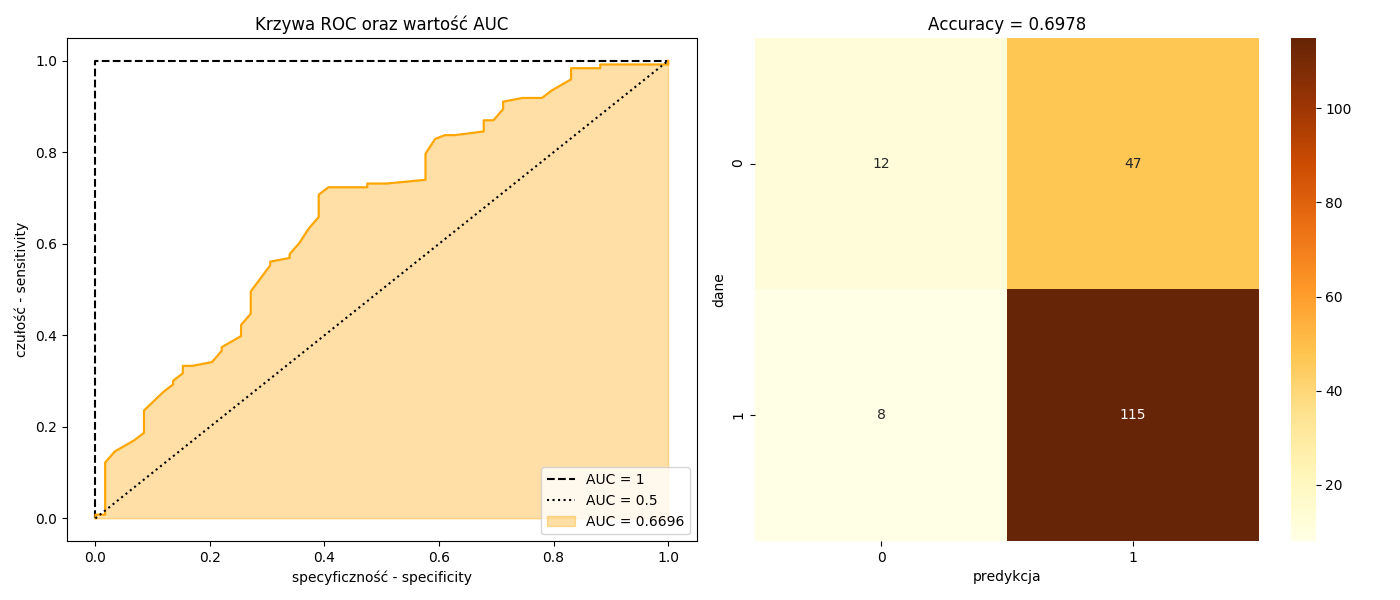
\includegraphics[width=1\linewidth]{roc} 

}

\caption{Krzywa ROC i tablica trafności prognoz.}\label{fig:roc}
\end{figure}

\hypertarget{R6}{%
\chapter{Rozkład ujemny dwumianowy}\label{R6}}

\begin{center}\rule{0.5\linewidth}{\linethickness}\end{center}

\hypertarget{R61}{%
\section{Funkcja gęstości}\label{R61}}

Rozkład ujemny dwumianowy (zwany też rozkładem Pascala) został zaimplementowany do funkcji \href{https://docs.scipy.org/doc/scipy/reference/generated/scipy.stats.nbinom.html}{\texttt{scipy.stats.nbinom}} i można go przedstawić za pomocą wzoru:
\begin{equation}
f(x\;|\;r,p)={x+r-1\choose r-1}p^r(1-p)^x,\quad x=0,1,...,\quad r\in N
\label{eq:ub01a}
\end{equation}
gdzie: \(r\) jest liczbą sukcesów, \(x\) jest liczbą niepowodzeń tj. liczba zdarzeń poprzedzających \(r\) sukcesów, a \(p\) jest prawdopodobieństwem niepowodzeń.

Do powyższego wzoru \eqref{eq:ub01a} można zastosować alternatywny zapis współczynnika dwumianu:
\begin{equation}
f(x\;|\;r,p)={x+r-1\choose x}p^r(1-p)^x,\quad x=0,1,...,\quad r>0
\label{eq:ub01b}
\end{equation}
dzięki któremu w rozkładzie ujemnym dwumianowym (zwanym też rozkładem Polya) można przyjąć, że parametr \(r>0\). Dodatkowo współczynnik dwumianowy można zapisać w oparciu o funkcję gamma:
\begin{equation}
f(x\;|\;r,p)=\frac{\Gamma(x+r)}{\Gamma(r)\Gamma(x+1)}p^r(1-p)^x,\quad x=0,1,...,\quad r>0
\label{eq:ub02}
\end{equation}
gdzie: \(E(X)=r(1-p)/p\) oraz \(V(X)=r(1-p)/p^2\).

\begin{Shaded}
\begin{Highlighting}[]
\ImportTok{import}\NormalTok{ scipy.stats }\ImportTok{as}\NormalTok{ stats}
\ImportTok{import}\NormalTok{ numpy }\ImportTok{as}\NormalTok{ np}
    
\NormalTok{x }\OperatorTok{=}\NormalTok{ stats.nbinom.rvs(n}\OperatorTok{=}\FloatTok{5.7}\NormalTok{, p}\OperatorTok{=}\FloatTok{0.3}\NormalTok{, size}\OperatorTok{=}\DecValTok{10000}\NormalTok{, random_state}\OperatorTok{=}\DecValTok{2305}\NormalTok{)}
\NormalTok{r }\OperatorTok{=}\NormalTok{ np.mean(x)}\OperatorTok{**}\DecValTok{2}\OperatorTok{/}\NormalTok{(np.var(x,ddof}\OperatorTok{=}\DecValTok{1}\NormalTok{)}\OperatorTok{-}\NormalTok{np.mean(x))}
\NormalTok{p }\OperatorTok{=}\NormalTok{ np.mean(x)}\OperatorTok{/}\NormalTok{np.var(x,ddof}\OperatorTok{=}\DecValTok{1}\NormalTok{)}
\BuiltInTok{print}\NormalTok{(}\StringTok{"MOM: r= }\SpecialCharTok{%.4f}\StringTok{, p= }\SpecialCharTok\NormalTok{ (r,p))}
\end{Highlighting}
\end{Shaded}

\begin{verbatim}
## MOM: r= 5.5556, p= 0.2948
\end{verbatim}

Jeżeli przyjmiemy, że parametr \(r=\phi\) oraz \(p=\frac{\phi}{\mu+\phi}\) to mieszanka rozkładu Poissona-Gamma będzie miała postać:
\begin{equation}
f(x\;|\;\mu,\phi)
=\frac{\Gamma(x+\phi)}{\Gamma(\phi)\Gamma(x+1)}\left(\frac{\phi}{\mu+\phi}\right)^{\phi}\left(\frac{\mu}{\mu+\phi}\right)^{x},\quad x=0,1,...,\quad \phi>0
\label{eq:ub03}
\end{equation}
gdzie: \(E(X)=\mu\) oraz \(V(X)=\mu+\phi^{-1}\mu^2\).

\begin{Shaded}
\begin{Highlighting}[]
\ImportTok{import}\NormalTok{ scipy.stats }\ImportTok{as}\NormalTok{ stats}
\ImportTok{import}\NormalTok{ numpy }\ImportTok{as}\NormalTok{ np}
\ImportTok{from}\NormalTok{ scipy.optimize }\ImportTok{import}\NormalTok{ minimize}

\KeywordTok{def}\NormalTok{ rn(mu, phi, n, rand):}
\NormalTok{    r }\OperatorTok{=}\NormalTok{ phi }\CommentTok{# phi_nb2}
\NormalTok{    p }\OperatorTok{=}\NormalTok{ r}\OperatorTok{/}\NormalTok{(mu}\OperatorTok{+}\NormalTok{r)}
    \ControlFlowTok{return}\NormalTok{ stats.nbinom.rvs(n}\OperatorTok{=}\NormalTok{r, p}\OperatorTok{=}\NormalTok{p, size}\OperatorTok{=}\NormalTok{n, random_state}\OperatorTok{=}\NormalTok{rand)}

\NormalTok{x }\OperatorTok{=}\NormalTok{ rn(mu }\OperatorTok{=} \FloatTok{1.5}\NormalTok{, phi }\OperatorTok{=} \DecValTok{5}\NormalTok{, n }\OperatorTok{=} \DecValTok{10000}\NormalTok{, rand }\OperatorTok{=} \DecValTok{2305}\NormalTok{)}
\NormalTok{mu }\OperatorTok{=}\NormalTok{ np.mean(x)}
\NormalTok{phi }\OperatorTok{=}\NormalTok{ np.mean(x)}\OperatorTok{**}\DecValTok{2}\OperatorTok{/}\NormalTok{(np.var(x,ddof}\OperatorTok{=}\DecValTok{1}\NormalTok{)}\OperatorTok{-}\NormalTok{np.mean(x))}
\BuiltInTok{print}\NormalTok{(}\StringTok{"MOM: mean= }\SpecialCharTok{%.4f}\StringTok{, phi_NB2= }\SpecialCharTok\NormalTok{ (mu,phi))}

\KeywordTok{def}\NormalTok{ L_nb2(par):}
\NormalTok{    phi }\OperatorTok{=}\NormalTok{ par[}\DecValTok{0}\NormalTok{]}
\NormalTok{    mu }\OperatorTok{=}\NormalTok{ par[}\DecValTok{1}\NormalTok{]}
\NormalTok{    logLik }\OperatorTok{=} \OperatorTok{-}\NormalTok{np.}\BuiltInTok{sum}\NormalTok{( stats.nbinom.logpmf(x, n}\OperatorTok{=}\NormalTok{phi, p}\OperatorTok{=}\NormalTok{phi}\OperatorTok{/}\NormalTok{(phi}\OperatorTok{+}\NormalTok{mu)) )}
    \ControlFlowTok{return}\NormalTok{(logLik)}

\NormalTok{initParams }\OperatorTok{=}\NormalTok{ [}\DecValTok{1}\NormalTok{,}\DecValTok{1}\NormalTok{]}
\NormalTok{res }\OperatorTok{=}\NormalTok{ minimize(L_nb2, initParams, method}\OperatorTok{=} \StringTok{"Nelder-Mead"}\NormalTok{)}
\BuiltInTok{print}\NormalTok{(}\StringTok{"MLE: mean= }\SpecialCharTok{%.4f}\StringTok{, phi_NB2= }\SpecialCharTok{%.4f}\StringTok{, logLik= }\SpecialCharTok\NormalTok{ (res.x[}\DecValTok{1}\NormalTok{],res.x[}\DecValTok{0}\NormalTok{],L_nb2(res.x)))}
\end{Highlighting}
\end{Shaded}

\begin{verbatim}
## MOM: mean= 1.5083, phi_NB2= 5.1984
## MLE: mean= 1.5083, phi_NB2= 5.1768, logLik= 16106.60
\end{verbatim}

Gdy do wzoru \eqref{eq:ub03} podstawimy \(\phi=\alpha^{-1}\) i dokonamy prostych przekształceń to otrzymamy:
\begin{equation}
f(x\;|\;\mu,\alpha)=\frac{\Gamma(x+\alpha^{-1})}{\Gamma(\alpha^{-1})\Gamma(x+1)}\left(\frac{1}{\alpha\mu+1}\right)^{\alpha^{-1}}\left(\frac{\alpha\mu}{\alpha\mu+1}\right)^x
\label{eq:ub04}
\end{equation}
gdzie: \(E(X)=\mu\) oraz \(V(X)=\mu+\alpha\mu^2\).

\begin{Shaded}
\begin{Highlighting}[]
\ImportTok{import}\NormalTok{ scipy.stats }\ImportTok{as}\NormalTok{ stats}
\ImportTok{import}\NormalTok{ numpy }\ImportTok{as}\NormalTok{ np}

\KeywordTok{def}\NormalTok{ rn(mu, alpha, n, rand):}
\NormalTok{    r }\OperatorTok{=} \DecValTok{1}\OperatorTok{/}\NormalTok{alpha }\CommentTok{# phi_nb2}
\NormalTok{    p }\OperatorTok{=}\NormalTok{ r}\OperatorTok{/}\NormalTok{(mu}\OperatorTok{+}\NormalTok{r)}
    \ControlFlowTok{return}\NormalTok{ stats.nbinom.rvs(n}\OperatorTok{=}\NormalTok{r, p}\OperatorTok{=}\NormalTok{p, size}\OperatorTok{=}\NormalTok{n, random_state}\OperatorTok{=}\NormalTok{rand)}

\NormalTok{x }\OperatorTok{=}\NormalTok{ rn(mu }\OperatorTok{=} \FloatTok{1.5}\NormalTok{, alpha }\OperatorTok{=} \DecValTok{9}\NormalTok{, n }\OperatorTok{=} \DecValTok{10000}\NormalTok{, rand }\OperatorTok{=} \DecValTok{2305}\NormalTok{)}
\NormalTok{mu }\OperatorTok{=}\NormalTok{ np.mean(x)}
\NormalTok{alpha }\OperatorTok{=}\NormalTok{ (np.var(x,ddof}\OperatorTok{=}\DecValTok{1}\NormalTok{)}\OperatorTok{-}\NormalTok{np.mean(x))}\OperatorTok{/}\NormalTok{np.mean(x)}\OperatorTok{**}\DecValTok{2}
\BuiltInTok{print}\NormalTok{(}\StringTok{"MOM: mean= }\SpecialCharTok{%.4f}\StringTok{, alpha_NB2= }\SpecialCharTok\NormalTok{ (mu,alpha))}
\end{Highlighting}
\end{Shaded}

\begin{verbatim}
## MOM: mean= 1.5355, alpha_NB2= 9.1284
\end{verbatim}

Po zlogarytmowaniu wyrażenia \eqref{eq:ub04} otrzymamy funkcję logarytmu wiarygodności o postaci:
\begin{equation}
L(x\;|\;\mu,\alpha)=\ln\Gamma(x+\alpha^{-1})-\ln\Gamma(\alpha^{-1})-\ln\Gamma(x+1)-\alpha^{-1}\ln(1+\alpha\mu)-x\ln(1+\alpha\mu)+x\ln(\alpha\mu)
\label{eq:ub05}
\end{equation}

\hypertarget{R62}{%
\section{Liniowy model ujemnej dwumianowej regresji}\label{R62}}

Do modelowania zmiennych licznikowych można stosować regresję Poissona jeśli zostało spełnione założenie równości średniej i wariancji. W przypadku wystąpienia zjawiska zawyżonej dyspersji tj. \(E(X)\leq V(X)\) nie można prawidłowo wyznaczyć błędów standardowych ocen parametrów. Rozwiązaniem tego problemu może być zastosowanie takich rozkładów które są przeznaczone do modelowania nadmiernie rozproszonych danych. Jedną z wielu propozycji \citep{pois2016} jest rozkład ujemny dwumianowy z liniową (NB1) lub kwadratową (NB2) zależnością między średnią a wariancją \citep{pois1998}:
\begin{equation}
V(X)=\mu+\alpha\mu^p
\label{eq:ub06}
\end{equation}

\begin{itemize}
\item
  model NB1 dla \(p=1\):
  \begin{equation}
  E[(y_i-\mu_i)^2]=\phi\mu_i\quad\longrightarrow\quad\phi = E[(y_i-\mu_i)^2/\mu_i]
  \label{eq:ub07}
  \end{equation}
  Estymator parametru \(\phi\) po zastosowaniu korekty:
  \begin{equation}
  \hat{\phi}_{\mathrm{NB1}}=\frac{1}{n-k}\sum_{i=1}^{n}\frac{(y_i-\hat{\mu}_i)^2}{\hat{\mu}_i}\quad\mathrm{gdzie}\quad\hat{\alpha}_{\mathrm{NB1}}=\hat{\phi}_{\mathrm{NB1}}-1
  \label{eq:ub08}
  \end{equation}
\item
  model NB2 dla \(p=2\):
  \begin{equation}
  E[(y_i-\mu_i)^2-\mu_i]=\alpha\mu_i^2\quad\longrightarrow\quad\alpha = E[\{(y_i-\mu_i)^2-\mu_i\}/\mu_i^2]
  \label{eq:ub09}
  \end{equation}
  Estymator parametru \(\alpha\) po zastosowaniu korekty:
  \begin{equation}
  \hat{\alpha}_{\mathrm{NB2}}=\frac{1}{n-k}\sum_{i=1}^{n}\frac{(y_i-\hat{\mu}_i)^2-\hat{\mu}_i}{\hat{\mu}^2_i}\quad\mathrm{gdzie}\quad\hat{\phi}_{\mathrm{NB2}}=1/\hat{\alpha}_{\mathrm{NB2}}
  \label{eq:ub10}
  \end{equation}
\end{itemize}

W modelu który uwzględnia nadmierną dyspersje (model quasi-Poissona) błędy standardowe są modyfikowane w oparciu o wzór:
\begin{equation}
SE_{Q}(\beta)=SE_{Pois}(\beta)\cdot \sqrt{\hat{\phi}_{\mathrm{NB1}}}
\label{eq:ub011}
\end{equation}
Warto podkreślić, że w równaniu \eqref{eq:ub011} jest wykorzystany estymator \(\hat{\phi}_{\mathrm{NB1}}\) który jest powszechnie stosowany do szacowania nadmiernej dyspersji w modelu Poissona \citep{glm1989}.
Dodajmy jeszcze, że estymator dyspersji \eqref{eq:ub08} można zapisać w alternatywny sposób:
\begin{equation}
\hat{\phi}_{\mathrm{NB1}}=\frac{\chi^2_P}{n-k}
\label{eq:ub012}
\end{equation}
gdzie: \(\chi^2_{P}\) to suma kwadratów reszt Pearsona która jest często stosowana do oceny dobroci dopasowania modelu. Reszty Pearsona wyznaczamy na bazie regresji Poissona za pomocą wzoru:
\begin{equation}
r_{i}^P=\frac{y_i-\hat{u}_i}{\sqrt{\hat{u}_i}}
\label{eq:ub013}
\end{equation}

Wykorzystanie funkcji \href{https://www.statsmodels.org/dev/generated/statsmodels.discrete.discrete_model.NegativeBinomial.html\#statsmodels.discrete.discrete_model.NegativeBinomial}{\texttt{statsmodels.discrete.discrete\_model.NegativeBinomial}} umożliwia oszacowanie modelu NB1 lub NB2 (opcja domyślna) oraz parametru \(\alpha\). Zastosowanie liniowego modelu ujemnej dwumianowej regresji zostanie zaprezentowane na przykładzie zestawu danych \href{https://stats.idre.ucla.edu/r/dae/negative-binomial-regression/}{\texttt{nb\_data}}.

\begin{Shaded}
\begin{Highlighting}[]
\ImportTok{import}\NormalTok{ pandas }\ImportTok{as}\NormalTok{ pd}
\ImportTok{import}\NormalTok{ statsmodels.api }\ImportTok{as}\NormalTok{ sm}
\ImportTok{import}\NormalTok{ patsy}
                  
\NormalTok{df }\OperatorTok{=}\NormalTok{ pd.read_stata(}\StringTok{'https://stats.idre.ucla.edu/stat/stata/dae/nb_data.dta'}\NormalTok{)}
\NormalTok{df[}\StringTok{'prog'}\NormalTok{].replace([}\FloatTok{1.0}\NormalTok{,}\FloatTok{2.0}\NormalTok{,}\FloatTok{3.0}\NormalTok{],[}\StringTok{'General'}\NormalTok{,}\StringTok{'Academic'}\NormalTok{,}\StringTok{'Vocational'}\NormalTok{],inplace}\OperatorTok{=}\VariableTok{True}\NormalTok{)}
\NormalTok{model }\OperatorTok{=} \StringTok{'daysabs ~ math + C(prog, Treatment(reference="General"))'}
\NormalTok{y, x }\OperatorTok{=}\NormalTok{ patsy.dmatrices(model, df, return_type}\OperatorTok{=}\StringTok{'dataframe'}\NormalTok{)}
\NormalTok{x.columns }\OperatorTok{=}\NormalTok{ [}\StringTok{'Intercept'}\NormalTok{, }\StringTok{'Academic'}\NormalTok{, }\StringTok{'Vocational'}\NormalTok{,}\StringTok{'math'}\NormalTok{]}
    
\NormalTok{nb }\OperatorTok{=}\NormalTok{ sm.NegativeBinomial(y,x,loglike_method}\OperatorTok{=}\StringTok{'nb2'}\NormalTok{).fit(disp}\OperatorTok{=}\DecValTok{0}\NormalTok{)}
\NormalTok{a }\OperatorTok{=}\NormalTok{ nb.params.values[}\DecValTok{4}\NormalTok{]}
\BuiltInTok{print}\NormalTok{(nb.summary())}
\BuiltInTok{print}\NormalTok{(}\StringTok{"}\CharTok{\textbackslash{}n}\StringTok{phi: "}\NormalTok{,}\BuiltInTok{round}\NormalTok{(}\DecValTok{1}\OperatorTok{/}\NormalTok{a, }\DecValTok{8}\NormalTok{), }\StringTok{", sqrt_phi: "}\NormalTok{, }\BuiltInTok{round}\NormalTok{((}\DecValTok{1}\OperatorTok{/}\NormalTok{a)}\OperatorTok{**}\FloatTok{0.5}\NormalTok{, }\DecValTok{8}\NormalTok{))}
\end{Highlighting}
\end{Shaded}

\begin{verbatim}
##                      NegativeBinomial Regression Results                      
## ==============================================================================
## Dep. Variable:                daysabs   No. Observations:                  314
## Model:               NegativeBinomial   Df Residuals:                      310
## Method:                           MLE   Df Model:                            3
## Date:                Mon, 19 Aug 2019   Pseudo R-squ.:                 0.03441
## Time:                        19:23:11   Log-Likelihood:                -865.63
## converged:                       True   LL-Null:                       -896.47
## Covariance Type:            nonrobust   LLR p-value:                 2.563e-13
## ==============================================================================
##                  coef    std err          z      P>|z|      [0.025      0.975]
## ------------------------------------------------------------------------------
## Intercept      2.6153      0.196     13.319      0.000       2.230       3.000
## Academic      -0.4408      0.183     -2.414      0.016      -0.799      -0.083
## Vocational    -1.2787      0.202     -6.331      0.000      -1.675      -0.883
## math          -0.0060      0.003     -2.390      0.017      -0.011      -0.001
## alpha          0.9683      0.100      9.729      0.000       0.773       1.163
## ==============================================================================
## 
## phi:  1.03271369 , sqrt_phi:  1.01622522
\end{verbatim}

Za pomocą wybranej pomocniczej regresji liniowej:
\begin{equation}
w_i =\hat{\alpha}_{\,\mathrm{NB1}}+\epsilon_i
\label{eq:ub014}
\end{equation}
\begin{equation}
w_i=\hat{\alpha}_{\,\mathrm{NB2}}\,\hat{u}_i+\epsilon_i
\label{eq:ub015}
\end{equation}
można weryfikować hipotezy statystyczne:
\begin{equation}
H_0:\;\alpha_{\,\mathrm{NB1}}=0\quad\mathrm{vs}\quad H_1:\;\alpha_{\,\mathrm{NB1}}\neq0
\label{eq:ub016}
\end{equation}
\begin{equation}
H_0:\;\alpha_{\,\mathrm{NB2}}=0\quad\mathrm{vs}\quad H_1:\;\alpha_{\,\mathrm{NB2}}\neq0
\label{eq:ub017}
\end{equation}
Warto podkreślić, że \(\phi_{\,\mathrm{NB1}}=\alpha_{\,\mathrm{NB1}}+1\) więc hipotezę \eqref{eq:ub016} można przedstawić jako:
\begin{equation}
H_0:\;\phi_{\,\mathrm{NB1}}=1\quad\mathrm{vs}\quad H_1:\;\phi_{\,\mathrm{NB1}}\neq1
\label{eq:ub018}
\end{equation}
Dodatkowo wyniki uzyskane za pomocą regresji \eqref{eq:ub014} są tożsame wynikami uzyskanymi na podstawie wzorów:
\begin{equation}
\hat{\alpha}_{\mathrm{NB1}}=E(w_i)\quad\mathrm{oraz}\quad SE_{\hat{\alpha}_{1NB}}=\sqrt{V(w_i)/n}
\label{eq:ub019}
\end{equation}
gdzie:
\begin{equation}
w_i=\frac{(y_i-\hat{u}_i)^2-y_i}{\hat{u}_i}
\label{eq:ub020}
\end{equation}

\begin{Shaded}
\begin{Highlighting}[]
\ImportTok{import}\NormalTok{ warnings}
\NormalTok{warnings.filterwarnings(}\StringTok{"ignore"}\NormalTok{)}

\ImportTok{import}\NormalTok{ pandas }\ImportTok{as}\NormalTok{ pd}
\ImportTok{import}\NormalTok{ statsmodels.api }\ImportTok{as}\NormalTok{ sm}
\ImportTok{import}\NormalTok{ patsy}
  
\NormalTok{df }\OperatorTok{=}\NormalTok{ pd.read_stata(}\StringTok{'https://stats.idre.ucla.edu/stat/stata/dae/nb_data.dta'}\NormalTok{)}
\NormalTok{df[}\StringTok{'prog'}\NormalTok{].replace([}\FloatTok{1.0}\NormalTok{,}\FloatTok{2.0}\NormalTok{,}\FloatTok{3.0}\NormalTok{],[}\StringTok{'General'}\NormalTok{,}\StringTok{'Academic'}\NormalTok{,}\StringTok{'Vocational'}\NormalTok{],inplace}\OperatorTok{=}\VariableTok{True}\NormalTok{)}
\NormalTok{model }\OperatorTok{=} \StringTok{'daysabs ~ math + C(prog, Treatment(reference="General"))'}
\NormalTok{y, x }\OperatorTok{=}\NormalTok{ patsy.dmatrices(model, df, return_type}\OperatorTok{=}\StringTok{'dataframe'}\NormalTok{)}
\NormalTok{x.columns }\OperatorTok{=}\NormalTok{ [}\StringTok{'Intercept'}\NormalTok{, }\StringTok{'Academic'}\NormalTok{, }\StringTok{'Vocational'}\NormalTok{,}\StringTok{'math'}\NormalTok{]}
      
\NormalTok{yp }\OperatorTok{=}\NormalTok{ sm.Poisson(y,x).fit(disp}\OperatorTok{=}\DecValTok{0}\NormalTok{).predict()}
\NormalTok{w }\OperatorTok{=}\NormalTok{ ((y[}\StringTok{'daysabs'}\NormalTok{]}\OperatorTok{-}\NormalTok{yp)}\OperatorTok{**}\DecValTok{2}\OperatorTok{-}\NormalTok{y[}\StringTok{'daysabs'}\NormalTok{])}\OperatorTok{/}\NormalTok{yp}
\NormalTok{n1 }\OperatorTok{=}\NormalTok{ sm.OLS(w,yp}\OperatorTok{*}\DecValTok{0}\OperatorTok{+}\DecValTok{1}\NormalTok{).fit(use_t}\OperatorTok{=}\DecValTok{1}\NormalTok{) }\CommentTok{# regresja OLS dla alpha_NB1}
\NormalTok{n1.model.data.xnames }\OperatorTok{=}\NormalTok{ [}\StringTok{'alpha_NB1'}\NormalTok{]}
\NormalTok{n2 }\OperatorTok{=}\NormalTok{ sm.OLS(w,yp).fit(use_t}\OperatorTok{=}\DecValTok{1}\NormalTok{)     }\CommentTok{# regresja OLS dla alpha_NB2}
\NormalTok{n2.model.data.xnames }\OperatorTok{=}\NormalTok{ [}\StringTok{'alpha_NB2'}\NormalTok{]}
\BuiltInTok{print}\NormalTok{(n1.summary().tables[}\DecValTok{1}\NormalTok{])}
\BuiltInTok{print}\NormalTok{(}\StringTok{"phi_NB1: "}\NormalTok{,n1.params.values[}\DecValTok{0}\NormalTok{]}\OperatorTok{+}\DecValTok{1}\NormalTok{,}\StringTok{'}\CharTok{\textbackslash{}n}\StringTok{'}\NormalTok{)}
\BuiltInTok{print}\NormalTok{(n2.summary().tables[}\DecValTok{1}\NormalTok{])}
\BuiltInTok{print}\NormalTok{(}\StringTok{"phi_NB2: "}\NormalTok{,}\DecValTok{1}\OperatorTok{/}\NormalTok{n2.params.values[}\DecValTok{0}\NormalTok{])}
\end{Highlighting}
\end{Shaded}

\begin{verbatim}
## ==============================================================================
##                  coef    std err          t      P>|t|      [0.025      0.975]
## ------------------------------------------------------------------------------
## alpha_NB1      5.5105      0.768      7.178      0.000       4.000       7.021
## ==============================================================================
## phi_NB1:  6.51052636765949 
## 
## ==============================================================================
##                  coef    std err          t      P>|t|      [0.025      0.975]
## ------------------------------------------------------------------------------
## alpha_NB2      0.7986      0.117      6.835      0.000       0.569       1.028
## ==============================================================================
## phi_NB2:  1.2522191233195814
\end{verbatim}

Funkcja \href{https://www.statsmodels.org/stable/generated/statsmodels.genmod.families.family.NegativeBinomial.html}{\texttt{statsmodels.genmod.families.family.NegativeBinomial}} umożliwia estymację modelu NB2 dla ustalonej wartości \(\alpha\). Warto zwrócić uwagę, że za pomocą tej funkcji możemy w sposób symulacyjny dobrać odpowienik parametr \(\alpha\). Dodajmy jeszcze, że do modelowania danych licznikowych można wykorzystać złożony rozkład Poissona--gamma który jest szczególnym przypadkiem rozkładu Tweedie:
\begin{equation}
E(X) = \mu \quad\mathrm{oraz}\quad Var(X) = \phi\mu^p
\label{eq:ub021}
\end{equation}
W zależności od wartości parametru kształtu \(p\) można otrzymać
kilka znanych rozkładów jako szczególne przypadki dystrybucji Tweedie:

\begin{itemize}
\item
  \(p = 0\) - rozkład normalny,
\item
  \(0 < p < 1\) - rozkład nie jest zdefiniowany,
\item
  \(p = 1\) - rozkład Poissona,
\item
  \(1 <p <2\) - rozkład Poissona--gamma,
\item
  \(p = 2\) - rozkład gamma,
\item
  \(2 <p <3\) - dodatnie rozkłady stabilne,
\item
  \(p = 3\) - odwrotny rozkład Gaussa / rozkład Walda,
\item
  \(p> 3\) - dodatnie rozkłady stabilne,
\item
  \(p =\infty\) - ekstremalne stabilne rozkłady.
\end{itemize}

\begin{Shaded}
\begin{Highlighting}[]
\ImportTok{import}\NormalTok{ numpy }\ImportTok{as}\NormalTok{ np}
\ImportTok{import}\NormalTok{ pandas }\ImportTok{as}\NormalTok{ pd}
\ImportTok{import}\NormalTok{ statsmodels.formula.api }\ImportTok{as}\NormalTok{ smf}
\ImportTok{import}\NormalTok{ statsmodels.api }\ImportTok{as}\NormalTok{ sm}

\NormalTok{df }\OperatorTok{=}\NormalTok{ pd.read_stata(}\StringTok{'https://stats.idre.ucla.edu/stat/stata/dae/nb_data.dta'}\NormalTok{)}
\NormalTok{df[}\StringTok{'prog'}\NormalTok{].replace([}\FloatTok{1.0}\NormalTok{,}\FloatTok{2.0}\NormalTok{,}\FloatTok{3.0}\NormalTok{],[}\StringTok{'General'}\NormalTok{,}\StringTok{'Academic'}\NormalTok{,}\StringTok{'Vocational'}\NormalTok{],inplace}\OperatorTok{=}\VariableTok{True}\NormalTok{)}
\NormalTok{model }\OperatorTok{=} \StringTok{'daysabs ~ math + C(prog, Treatment(reference="General"))'}
\NormalTok{B }\OperatorTok{=} \DecValTok{100}
\NormalTok{X }\OperatorTok{=}\NormalTok{ np.linspace(}\FloatTok{1.0001}\NormalTok{,}\FloatTok{1.9999}\NormalTok{,B)}
\NormalTok{n }\OperatorTok{=}\NormalTok{ [smf.glm(model, data}\OperatorTok{=}\NormalTok{df,}\OperatorTok{\textbackslash{}}
\NormalTok{     family }\OperatorTok{=}\NormalTok{ sm.families.Tweedie(link }\OperatorTok{=}\NormalTok{ sm.families.links.log, var_power}\OperatorTok{=}\NormalTok{i)).fit() }\ControlFlowTok{for}\NormalTok{ i }\KeywordTok{in}\NormalTok{ X]}
\NormalTok{res }\OperatorTok{=}\NormalTok{ [n[i].deviance }\ControlFlowTok{for}\NormalTok{ i }\KeywordTok{in} \BuiltInTok{range}\NormalTok{(B)]}
\NormalTok{sol }\OperatorTok{=}\NormalTok{ n[np.argmin(res)]}
\NormalTok{sol.model.data.xnames }\OperatorTok{=}\NormalTok{ [}\StringTok{'Inercept'}\NormalTok{,}\StringTok{'Academic'}\NormalTok{,}\StringTok{'Vocational'}\NormalTok{,}\StringTok{'math'}\NormalTok{]}
\BuiltInTok{print}\NormalTok{(sol.summary())}
\BuiltInTok{print}\NormalTok{(}\StringTok{"}\CharTok{\textbackslash{}n}\StringTok{p: "}\NormalTok{,X[np.argmin(res)])}
\end{Highlighting}
\end{Shaded}

\begin{verbatim}
##                  Generalized Linear Model Regression Results                  
## ==============================================================================
## Dep. Variable:                daysabs   No. Observations:                  314
## Model:                            GLM   Df Residuals:                      310
## Model Family:                 Tweedie   Df Model:                            3
## Link Function:                    log   Scale:                          2.3160
## Method:                          IRLS   Log-Likelihood:                    nan
## Date:                Mon, 19 Aug 2019   Deviance:                       902.82
## Time:                        19:23:15   Pearson chi2:                     718.
## No. Iterations:                    10                                         
## Covariance Type:            nonrobust                                         
## ==============================================================================
##                  coef    std err          z      P>|z|      [0.025      0.975]
## ------------------------------------------------------------------------------
## Inercept       2.6258      0.192     13.699      0.000       2.250       3.001
## Academic      -0.4410      0.178     -2.484      0.013      -0.789      -0.093
## Vocational    -1.2779      0.203     -6.305      0.000      -1.675      -0.881
## math          -0.0062      0.003     -2.423      0.015      -0.011      -0.001
## ==============================================================================
## 
## p:  1.6363363636363637
\end{verbatim}

\hypertarget{R7}{%
\chapter{Błąd standardowy estymatora}\label{R7}}

\hypertarget{R71}{%
\section{Średnia}\label{R71}}

Średnia jest parametrem który ma swoje zastosowanie dla rozkładów symetrycznych.
Błąd standardowy estymatora średniej \(\bar{x}\) można zapisać za pomocą wzoru:
\begin{equation}
SE_{\bar{x}}=\sqrt{s^2/n}
\label{eq:se01}
\end{equation}
gdzie: \(s^2\) to nieobciążony estymator wariancji: \(\sum_{i=1}^{n}(x_i-\bar{x})^2/(n-1)\) oraz \(\bar{x}\) to estymator średniej czyli \(\sum_{i=1}^{n}x_i/n\). Dodatkowo \(x_i\) to kolejne elementy próby a \(n\) to liczebność próby.

\begin{Shaded}
\begin{Highlighting}[]
\ImportTok{import}\NormalTok{ numpy }\ImportTok{as}\NormalTok{ np}
\ImportTok{import}\NormalTok{ scipy.stats }\ImportTok{as}\NormalTok{ stats}

\NormalTok{y }\OperatorTok{=}\NormalTok{ stats.norm.rvs(size}\OperatorTok{=}\DecValTok{300}\NormalTok{,scale}\OperatorTok{=}\DecValTok{3}\NormalTok{,random_state}\OperatorTok{=}\DecValTok{4101}\NormalTok{)}

\NormalTok{MU }\OperatorTok{=}\NormalTok{ np.mean(y)}
\NormalTok{SE_mu }\OperatorTok{=}\NormalTok{ np.sqrt(np.var(y, ddof}\OperatorTok{=}\DecValTok{1}\NormalTok{)}\OperatorTok{/}\BuiltInTok{len}\NormalTok{(y))}
\NormalTok{conf }\OperatorTok{=}\NormalTok{ [ stats.norm.ppf(i, loc}\OperatorTok{=}\NormalTok{MU, scale}\OperatorTok{=}\NormalTok{SE_mu) }\ControlFlowTok{for}\NormalTok{ i }\KeywordTok{in}\NormalTok{ [}\FloatTok{0.025}\NormalTok{,}\FloatTok{0.975}\NormalTok{] ]}
\NormalTok{p }\OperatorTok{=}\NormalTok{ stats.norm.cdf(}\DecValTok{0}\NormalTok{, MU, SE_mu)}

\BuiltInTok{print}\NormalTok{(}\StringTok{"średnia:"}\NormalTok{,MU,}\StringTok{", błąd:"}\NormalTok{,SE_mu)}
\BuiltInTok{print}\NormalTok{(}\StringTok{"95% przedział ufności:"}\NormalTok{,conf)}
\BuiltInTok{print}\NormalTok{(}\StringTok{"}\CharTok{\textbackslash{}n}\StringTok{H0: mu = 0 vs. H1: mu != 0"}\NormalTok{)}
\BuiltInTok{print}\NormalTok{(}\StringTok{"p-wartość:"}\NormalTok{,}\DecValTok{2}\OperatorTok{*}\BuiltInTok{min}\NormalTok{(p,}\DecValTok{1}\OperatorTok{-}\NormalTok{p))}
\end{Highlighting}
\end{Shaded}

\begin{verbatim}
## średnia: 0.2707762688190597 , błąd: 0.16529559742815514
## 95% przedział ufności: [-0.053197148943156025, 0.5947496865812754]
## 
## H0: mu = 0 vs. H1: mu != 0
## p-wartość: 0.1013938313336142
\end{verbatim}

Ponieważ badamy hipotezę zerową \(H_0:\mu=0\) więc takie same wyniki można uzyskać za pomocą funkcji regresji liniowej.

\begin{Shaded}
\begin{Highlighting}[]
\ImportTok{from}\NormalTok{ scipy }\ImportTok{import}\NormalTok{ stats}
\ImportTok{import}\NormalTok{ pandas }\ImportTok{as}\NormalTok{ pd}

\NormalTok{df }\OperatorTok{=}\NormalTok{ pd.DataFrame(data}\OperatorTok{=}\NormalTok{\{}\StringTok{'y'}\NormalTok{:stats.norm.rvs(size}\OperatorTok{=}\DecValTok{300}\NormalTok{,scale}\OperatorTok{=}\DecValTok{3}\NormalTok{,random_state}\OperatorTok{=}\DecValTok{4101}\NormalTok{)\})}

\ImportTok{import}\NormalTok{ statsmodels.formula.api }\ImportTok{as}\NormalTok{ smf}

\NormalTok{m }\OperatorTok{=}\NormalTok{ smf.glm(}\StringTok{'y ~ 1'}\NormalTok{, data}\OperatorTok{=}\NormalTok{df).fit().summary().tables[}\DecValTok{1}\NormalTok{]}
\BuiltInTok{print}\NormalTok{(m)}
\end{Highlighting}
\end{Shaded}

\begin{verbatim}
## ==============================================================================
##                  coef    std err          z      P>|z|      [0.025      0.975]
## ------------------------------------------------------------------------------
## Intercept      0.2708      0.165      1.638      0.101      -0.053       0.595
## ==============================================================================
\end{verbatim}

\hypertarget{R72}{%
\section{Proporcja}\label{R72}}

Obliczenie proporcji na podstawie próby binarnej czyli zawierającej tylko zera (porażka) i jedynki (sukces) sprowadza się do wyznaczenia średniej. Przykładem może być zmienna \texttt{plec} gdzie: \texttt{0} - kobieta, \texttt{1} - mężczyzna.
Błąd standardowy dla oszacowanej frakcji \(\hat{p}\) jest dany wzorem:
\begin{equation}
SE_{\hat{p}}=\sqrt{\big(\hat{p}(1-\hat{p})\big)/n}\quad\mbox{gdzie}\quad \hat{p}\in(0,1)
\label{eq:se02}
\end{equation}

\begin{Shaded}
\begin{Highlighting}[]
\ImportTok{from}\NormalTok{ scipy }\ImportTok{import}\NormalTok{ stats}
\ImportTok{import}\NormalTok{ numpy }\ImportTok{as}\NormalTok{ np}

\NormalTok{y }\OperatorTok{=}\NormalTok{ stats.binom.rvs(n}\OperatorTok{=}\DecValTok{1}\NormalTok{, p}\OperatorTok{=}\FloatTok{0.3}\NormalTok{, loc}\OperatorTok{=}\DecValTok{0}\NormalTok{, size}\OperatorTok{=}\DecValTok{50}\NormalTok{, random_state}\OperatorTok{=}\DecValTok{2305}\NormalTok{)}

\NormalTok{P }\OperatorTok{=}\NormalTok{ np.mean(y)}
\NormalTok{SE_pw }\OperatorTok{=}\NormalTok{ np.sqrt((P}\OperatorTok{*}\NormalTok{(}\DecValTok{1}\OperatorTok{-}\NormalTok{P))}\OperatorTok{/}\BuiltInTok{len}\NormalTok{(y))}
\NormalTok{conf }\OperatorTok{=}\NormalTok{ [ stats.norm.ppf(i, loc}\OperatorTok{=}\NormalTok{P, scale}\OperatorTok{=}\NormalTok{SE_pw) }\ControlFlowTok{for}\NormalTok{ i }\KeywordTok{in}\NormalTok{ [}\FloatTok{0.025}\NormalTok{,}\FloatTok{0.975}\NormalTok{] ]}
\NormalTok{p }\OperatorTok{=}\NormalTok{ stats.norm.cdf(}\FloatTok{0.5}\NormalTok{, P, SE_pw)}

\BuiltInTok{print}\NormalTok{(}\StringTok{"proporcja:"}\NormalTok{,P,}\StringTok{", błąd:"}\NormalTok{,SE_pw)}
\BuiltInTok{print}\NormalTok{(}\StringTok{"95% przedział ufności:"}\NormalTok{,conf)}
\BuiltInTok{print}\NormalTok{(}\StringTok{"}\CharTok{\textbackslash{}n}\StringTok{H0: p = 0.5 vs. H1: p != 0.5"}\NormalTok{)}
\BuiltInTok{print}\NormalTok{(}\StringTok{"p-wartość:"}\NormalTok{,}\DecValTok{2}\OperatorTok{*}\BuiltInTok{min}\NormalTok{(p,}\DecValTok{1}\OperatorTok{-}\NormalTok{p))}
\end{Highlighting}
\end{Shaded}

\begin{verbatim}
## proporcja: 0.28 , błąd: 0.06349803146555018
## 95% przedział ufności: [0.15554614523833055, 0.4044538547616695]
## 
## H0: p = 0.5 vs. H1: p != 0.5
## p-wartość: 0.0005308739249216821
\end{verbatim}

Więcej procedur budowy przedziału ufności dla proporcji jest zaimplementowanych do funkcji
\href{https://www.statsmodels.org/stable/generated/statsmodels.stats.proportion.proportion_confint.html\#statsmodels.stats.proportion.proportion_confint}{\texttt{statsmodels.stats.proportion.proportion\_confint}} w której metoda Walda \eqref{eq:se02} jest rozwiązaniem domyślnym.

\begin{Shaded}
\begin{Highlighting}[]
\ImportTok{from}\NormalTok{ statsmodels.stats.proportion }\ImportTok{import}\NormalTok{ proportion_confint}
\ImportTok{from}\NormalTok{ scipy }\ImportTok{import}\NormalTok{ stats}

\NormalTok{y }\OperatorTok{=}\NormalTok{ stats.binom.rvs(n}\OperatorTok{=}\DecValTok{1}\NormalTok{, p}\OperatorTok{=}\FloatTok{0.3}\NormalTok{, loc}\OperatorTok{=}\DecValTok{0}\NormalTok{, size}\OperatorTok{=}\DecValTok{50}\NormalTok{, random_state}\OperatorTok{=}\DecValTok{2305}\NormalTok{)}

\BuiltInTok{print}\NormalTok{(proportion_confint(}\BuiltInTok{sum}\NormalTok{(y), }\DecValTok{50}\NormalTok{, alpha}\OperatorTok{=}\FloatTok{0.05}\NormalTok{, method}\OperatorTok{=}\StringTok{'normal'}\NormalTok{))}
\end{Highlighting}
\end{Shaded}

\begin{verbatim}
## (0.15554614523833055, 0.4044538547616695)
\end{verbatim}

\hypertarget{R73}{%
\section{Mediana}\label{R73}}

Jednym z bardziej popularnych odpornych estymatorów średniej jest mediana czyli drugi kwartyl który dzieli uporządkowany rosnąco zbiór obserwacji \(x\) na połowę. Wartość środkowa to \(x_{(n+1)/2}\) lub \((x_{n/2}+x_{(n/2 )+1})/2\) odpowiednio dla nieparzystej i parzystej liczebności danych.
Do estymacji przedziałowej mediany często jest wykorzystywany błąd standardowy:
\begin{equation}
SE_{np_0}=\sqrt{p_0(1-p_0)\cdot n}\quad\mbox{gdzie}\quad p_0=0.5
\label{eq:se03}
\end{equation}
Po uporządkowaniu rosnąco danych wybieramy dwa elementy o indeksach \(v_1\) i \(v_2\) które wyznaczają dolną \(x_{v_1}\) i górną \(x_{v_2}\) granicę przedziału ufności gdzie:
\begin{equation}
v_1=\lceil \Phi^{-1}(\alpha/2,\;np_0,SE_{np_0})\rceil,\quad v_2=\lceil  \Phi^{-1}(1-\alpha/2,\;np_0,SE_{np_0})\rceil
\label{eq:se04}
\end{equation}
Dodajmy, że dla mediany czyli \(p_0=0.5\) otrzymamy \(np_0=n/2\) oraz \(SE_{np_0}=\sqrt{n/4}\).

W innym rozwiązaniu \citep{ms1984} wykorzystywany jest błąd standardowy mediany dany wzorem:
\begin{equation}
SE_{\hat{m}}=\frac{x_{n-k+1}-x_{k}}{2\cdot z_{\,0.995}}\quad \mathrm{dla}\quad k=\frac{n+1}{2}-z_{\,0.995}\cdot\sqrt{\frac{n}{4}}
\label{eq:se05}
\end{equation}
gdzie kwantyle z rozkładu normalnego: \(\Phi^{-1}(\alpha/2,\;\hat{m},SE_{\hat{m}})\) oraz \(\Phi^{-1}(1-\alpha/2,\;\hat{m},SE_{\hat{m}})\)
to odpowiednio dolna i górna granica przedziału ufności.

Zwróćmy uwagę, że powyższe metody nie uwzględniają wartości wiązanych a więc są przeznaczone dla danych ciągłych. W artykule \citep{iwasaki2005} jest przedstawiona metoda która uwzględnia występowanie duplikatów:
\begin{equation}
v=\left[n/2-z_{1-\alpha/2}\cdot \sqrt{n/4}\right]+1,\quad v^{\prime}=\left[n/2-z_{1-\alpha/2}\cdot\sqrt{n/4}+0,5\right]+1
\label{eq:se06}
\end{equation}
\begin{equation}
\begin{aligned}
x_{v}\,,\;x_{n+1-v}
&
&
\textrm{dla}\quad
&
v=v^{\prime}\\[0.0in]
(x_{v-1}+x_{v})/2\,,\;(x_{n+1-v}+x_{(n+1-v)+1})/2
&
&
\textrm{dla}\quad
&
v=v^{\prime}-1
\end{aligned}
\label{eq:se07}
\end{equation}

W literaturze \citep{wilcox2017} można znaleźć jeszcze wiele innych propozycji. Za przykład może posłużyć estymator Harrella--Davisa \citep{hd1982} dla mediany lub wybranych kwantyli:
\begin{equation}
HD_{q}=\sum_{i=1}^{n}\left[\Big(B(i/n,\,a,\,b)-B((i-1)/n,\,a,\,b)\Bigr)x_{i}\right]
\label{eq:se08}
\end{equation}
z wykorzystaniem rozkładu beta (patrz rozdział \ref{R4}):
\begin{equation}
B(t,a,b)=\int_{0}^{t}\frac{\Gamma(a+b)}{\Gamma(a)\Gamma(b)}x^{a-1}(1-x)^{b-1}\;dx
\label{eq:se09}
\end{equation}
gdzie: \(a=(n+1)q\) oraz \(b=(n+1)(q-1)\) dla \(q=0.5\) w przypadku drugiego kwartyla czyli mediany.
Błąd standardowy estymatora mediany Harrella--Davisa można obliczyć za pomocą funkcji \href{https://docs.scipy.org/doc/scipy/reference/generated/scipy.stats.mstats.hdquantiles_sd.html\#scipy.stats.mstats.hdquantiles_sd}{\texttt{scipy.stats.mstats.hdquantiles\_sd}} do której zaimplementowano metodę jackknife. Inne rozwiązanie to wykorzystanie metody bootstrap (patrz podrozdział \ref{R78}) w której można wykorzystać estymator Harrella--Davisa zaimplementowany w funkcji \href{https://docs.scipy.org/doc/scipy/reference/generated/scipy.stats.mstats.hdquantiles.html}{\texttt{scipy.stats.mstats.hdquantiles}}.

\begin{Shaded}
\begin{Highlighting}[]
\ImportTok{from}\NormalTok{ scipy }\ImportTok{import}\NormalTok{ stats}

\NormalTok{y }\OperatorTok{=}\NormalTok{ stats.norm.rvs(size}\OperatorTok{=}\DecValTok{300}\NormalTok{,scale}\OperatorTok{=}\DecValTok{3}\NormalTok{,random_state}\OperatorTok{=}\DecValTok{4101}\NormalTok{)}

\NormalTok{MD }\OperatorTok{=}\NormalTok{ stats.mstats.hdquantiles(y,[}\FloatTok{0.5}\NormalTok{])[}\DecValTok{0}\NormalTok{]}
\NormalTok{SE_md }\OperatorTok{=}\NormalTok{ stats.mstats.hdquantiles_sd(y,[}\FloatTok{0.5}\NormalTok{])[}\DecValTok{0}\NormalTok{]}
\NormalTok{conf }\OperatorTok{=}\NormalTok{ [ stats.norm.ppf(i, loc}\OperatorTok{=}\NormalTok{MD, scale}\OperatorTok{=}\NormalTok{SE_md) }\ControlFlowTok{for}\NormalTok{ i }\KeywordTok{in}\NormalTok{ [}\FloatTok{0.025}\NormalTok{,}\FloatTok{0.975}\NormalTok{] ]}
\NormalTok{p }\OperatorTok{=}\NormalTok{ stats.norm.cdf(}\DecValTok{0}\NormalTok{, MD, SE_md)}

\BuiltInTok{print}\NormalTok{(}\StringTok{"medianaHD:"}\NormalTok{,MD,}\StringTok{", błąd:"}\NormalTok{,SE_md)}
\BuiltInTok{print}\NormalTok{(}\StringTok{"95% przedział ufności:"}\NormalTok{,conf)}
\BuiltInTok{print}\NormalTok{(}\StringTok{"}\CharTok{\textbackslash{}n}\StringTok{H0: md = 0 vs. H1: md != 0"}\NormalTok{)}
\BuiltInTok{print}\NormalTok{(}\StringTok{"p-wartość:"}\NormalTok{,}\DecValTok{2}\OperatorTok{*}\BuiltInTok{min}\NormalTok{(p,}\DecValTok{1}\OperatorTok{-}\NormalTok{p))}
\end{Highlighting}
\end{Shaded}

\begin{verbatim}
## medianaHD: 0.30109081321402076 , błąd: 0.1584119409852424
## 95% przedział ufności: [-0.009390885838138907, 0.6115725122661804]
## 
## H0: md = 0 vs. H1: md != 0
## p-wartość: 0.05734360449353051
\end{verbatim}

\hypertarget{R74}{%
\section{Wariancja}\label{R74}}

Błąd standardowy estymatora wariancji \citep{asym2009} można obliczyć za pomocą wzoru:
\begin{equation}
SE_{s^2}=\sqrt{S^2/n}
\label{eq:se11}
\end{equation}
gdzie \(S^2\) to nieobciążony estymator wariancji dla zmiennej \(z_i=(x_i-\bar{x})^2\).

\begin{Shaded}
\begin{Highlighting}[]
\ImportTok{from}\NormalTok{ scipy }\ImportTok{import}\NormalTok{ stats}
\ImportTok{import}\NormalTok{ numpy }\ImportTok{as}\NormalTok{ np}

\NormalTok{y }\OperatorTok{=}\NormalTok{ stats.norm.rvs(size}\OperatorTok{=}\DecValTok{300}\NormalTok{,scale}\OperatorTok{=}\DecValTok{3}\NormalTok{,random_state}\OperatorTok{=}\DecValTok{4101}\NormalTok{)}

\NormalTok{V }\OperatorTok{=}\NormalTok{ np.var(y,ddof}\OperatorTok{=}\DecValTok{1}\NormalTok{)}
\NormalTok{z }\OperatorTok{=}\NormalTok{ (y}\OperatorTok{-}\NormalTok{np.mean(y))}\OperatorTok{**}\DecValTok{2}
\NormalTok{SE_v }\OperatorTok{=}\NormalTok{ np.sqrt(np.var(z,ddof}\OperatorTok{=}\DecValTok{1}\NormalTok{)}\OperatorTok{/}\BuiltInTok{len}\NormalTok{(z))}
\NormalTok{conf }\OperatorTok{=}\NormalTok{ [ stats.norm.ppf(i, loc}\OperatorTok{=}\NormalTok{V, scale}\OperatorTok{=}\NormalTok{SE_v) }\ControlFlowTok{for}\NormalTok{ i }\KeywordTok{in}\NormalTok{ [}\FloatTok{0.025}\NormalTok{,}\FloatTok{0.975}\NormalTok{] ]}
\NormalTok{p }\OperatorTok{=}\NormalTok{ stats.norm.cdf(}\DecValTok{10}\NormalTok{, V, SE_v)}

\BuiltInTok{print}\NormalTok{(}\StringTok{"wariancja:"}\NormalTok{,V,}\StringTok{", błąd:"}\NormalTok{,SE_v)}
\BuiltInTok{print}\NormalTok{(}\StringTok{"95% przedział ufności:"}\NormalTok{,conf)}
\BuiltInTok{print}\NormalTok{(}\StringTok{"}\CharTok{\textbackslash{}n}\StringTok{H0: var = 10 vs. H1: var != 10"}\NormalTok{)}
\BuiltInTok{print}\NormalTok{(}\StringTok{"p-wartość:"}\NormalTok{,}\DecValTok{2}\OperatorTok{*}\BuiltInTok{min}\NormalTok{(p,}\DecValTok{1}\OperatorTok{-}\NormalTok{p))}
\end{Highlighting}
\end{Shaded}

\begin{verbatim}
## wariancja: 8.19679035873922 , błąd: 0.6734837212813637
## 95% przedział ufności: [6.876786520853734, 9.516794196624705]
## 
## H0: var = 10 vs. H1: var != 10
## p-wartość: 0.007418799795601672
\end{verbatim}

Inne rozwiązanie \citep{FK2016} jest przedstawione poniżej:

\begin{equation}
SE_{var}=\sqrt{\left(\frac{1}{2(n-2)} +\frac{1}{2n}-\frac{2}{n - 3}\right) v^2 + 
        \left(\frac{3}{n-3}-\frac{2}{n-2}\right) m_4}
\label{eq:se12}
\end{equation}
gdzie: \(m_4=\sum_{i=1}^{n}(x_i-\bar{x})^4/n\) to czwarty moment centralny oraz \(v=\sum_{i-1}^{n}(x_i-\bar{x})^2/(n-1)\) to nieobciążony estymator wariancji.

\begin{Shaded}
\begin{Highlighting}[]
\ImportTok{from}\NormalTok{ scipy }\ImportTok{import}\NormalTok{ stats}
\ImportTok{import}\NormalTok{ numpy }\ImportTok{as}\NormalTok{ np}

\NormalTok{y }\OperatorTok{=}\NormalTok{ stats.norm.rvs(size}\OperatorTok{=}\DecValTok{300}\NormalTok{,scale}\OperatorTok{=}\DecValTok{3}\NormalTok{,random_state}\OperatorTok{=}\DecValTok{4101}\NormalTok{)}

\NormalTok{n }\OperatorTok{=} \BuiltInTok{len}\NormalTok{(y)}
\NormalTok{v2 }\OperatorTok{=}\NormalTok{ np.var(y,ddof}\OperatorTok{=}\DecValTok{1}\NormalTok{)}\OperatorTok{**}\DecValTok{2}
\NormalTok{m4 }\OperatorTok{=}\NormalTok{ stats.moment(y, moment}\OperatorTok{=}\DecValTok{4}\NormalTok{)}
\NormalTok{SE_v }\OperatorTok{=}\NormalTok{ np.sqrt((}\DecValTok{1}\OperatorTok{/}\NormalTok{(}\DecValTok{2}\OperatorTok{*}\NormalTok{n}\DecValTok{-4}\NormalTok{)}\OperatorTok{+}\DecValTok{1}\OperatorTok{/}\NormalTok{(}\DecValTok{2}\OperatorTok{*}\NormalTok{n)}\OperatorTok{-}\DecValTok{2}\OperatorTok{/}\NormalTok{(n}\DecValTok{-3}\NormalTok{))}\OperatorTok{*}\NormalTok{v2}\OperatorTok{+}\NormalTok{(}\DecValTok{3}\OperatorTok{/}\NormalTok{(n}\DecValTok{-3}\NormalTok{)}\OperatorTok{-}\DecValTok{2}\OperatorTok{/}\NormalTok{(n}\DecValTok{-2}\NormalTok{))}\OperatorTok{*}\NormalTok{m4)}
\BuiltInTok{print}\NormalTok{(}\StringTok{"wariancja:"}\NormalTok{,v2}\OperatorTok{**}\FloatTok{0.5}\NormalTok{,}\StringTok{", błąd:"}\NormalTok{,SE_v)}
\end{Highlighting}
\end{Shaded}

\begin{verbatim}
## wariancja: 8.19679035873922 , błąd: 0.6768982673783448
\end{verbatim}

\hypertarget{R75}{%
\section{Średnia ucięta}\label{R75}}

W przypadku gdy dane nie pochodzą z rozkładu normalnego (np. gdy rozkład jest skośny, w danych występują obserwacje odstające itp.) wnioskowanie o populacji z wykorzystaniem średniej nie jest dobrym wyborem. Jednym z możliwych rozwiązań jest zweryfikowanie hipotezy statystycznej dotyczącej średniej uciętej \citep{tmc1963} w oparciu o rozkład t-Studenta ze stopniami swobody \(df=n-2\lfloor n G \rfloor -1\). Estymator średniej uciętej jest obliczany na podstawie próbki z której została usunięta pewna frakcja skrajnych obserwacji a jego błąd standardowy jest dany wzorem:
\begin{equation}
SE_{\bar{x}_t}=s_w/(1-2G)\sqrt{n}
\label{eq:se10}
\end{equation}
gdzie: \(sw\) to odchylenie standardowe obliczone na podstawie próbki poddanej procesowi winsoryzacji.

\begin{Shaded}
\begin{Highlighting}[]
\ImportTok{from}\NormalTok{ scipy }\ImportTok{import}\NormalTok{ stats}
\ImportTok{import}\NormalTok{ numpy }\ImportTok{as}\NormalTok{ np}

\NormalTok{y }\OperatorTok{=}\NormalTok{ stats.norm.rvs(size}\OperatorTok{=}\DecValTok{300}\NormalTok{,scale}\OperatorTok{=}\DecValTok{3}\NormalTok{,random_state}\OperatorTok{=}\DecValTok{4101}\NormalTok{)}

\NormalTok{tMU }\OperatorTok{=}\NormalTok{ stats.mstats.trimmed_mean(y,limits}\OperatorTok{=}\NormalTok{(}\FloatTok{0.2}\NormalTok{,}\FloatTok{0.2}\NormalTok{))}
\NormalTok{SE_tmu }\OperatorTok{=}\NormalTok{ stats.mstats.trimmed_stde(y,limits}\OperatorTok{=}\NormalTok{(}\FloatTok{0.2}\NormalTok{,}\FloatTok{0.2}\NormalTok{))}
\NormalTok{conf }\OperatorTok{=}\NormalTok{ stats.mstats.trimmed_mean_ci(y, limits}\OperatorTok{=}\NormalTok{(}\FloatTok{0.2}\NormalTok{, }\FloatTok{0.2}\NormalTok{))}
\NormalTok{df }\OperatorTok{=} \BuiltInTok{len}\NormalTok{(y) }\OperatorTok{-} \DecValTok{2} \OperatorTok{*}\NormalTok{ np.floor(}\FloatTok{0.2} \OperatorTok{*} \BuiltInTok{len}\NormalTok{(y)) }\OperatorTok{-} \DecValTok{1}
\NormalTok{p }\OperatorTok{=}\NormalTok{ stats.t.cdf(}\DecValTok{0}\NormalTok{, df, tMU, SE_tmu)}

\BuiltInTok{print}\NormalTok{(}\StringTok{"średnia ucięta:"}\NormalTok{,tMU,}\StringTok{", błąd:"}\NormalTok{,SE_tmu)}
\BuiltInTok{print}\NormalTok{(}\StringTok{"95% przedział ufności:"}\NormalTok{,conf)}
\BuiltInTok{print}\NormalTok{(}\StringTok{"}\CharTok{\textbackslash{}n}\StringTok{H0: tmu = 0 vs. H1: tmu != 0"}\NormalTok{)}
\BuiltInTok{print}\NormalTok{(}\StringTok{"p-wartość:"}\NormalTok{,}\DecValTok{2}\OperatorTok{*}\BuiltInTok{min}\NormalTok{(p,}\DecValTok{1}\OperatorTok{-}\NormalTok{p))}
\end{Highlighting}
\end{Shaded}

\begin{verbatim}
## średnia ucięta: 0.2929142000036129 , błąd: 0.17589712092651877
## 95% przedział ufności: [-0.05418454  0.64001294]
## 
## H0: tmu = 0 vs. H1: tmu != 0
## p-wartość: 0.09761041405364616
\end{verbatim}

Warto dodać, że dla parametru ucięcia \(G\) równego 0 wynik będzie tożsamy z testem t-Studenta który został zaimplementowany do funkcji \href{https://docs.scipy.org/doc/scipy/reference/generated/scipy.stats.ttest_1samp.html}{\texttt{scipy.stats.ttest\_1samp}}.

\hypertarget{R76}{%
\section{Skośność}\label{R76}}

W rozkładzie normalnym (rozkład symetryczny) parametr skośności jest równy zero. Wartość tego parametru może być większa lub mniejsza od zera dla rozkładu odpowiednio prawostronnie skośnego lub lewostronnie skośnego. Dla podstawowej wersji parametru skośności \(g1=m_3/m_2^{3/2}\) bład standardowy można zapisać za pomocą wzoru:
\begin{equation}
SE_{g1}=\sqrt{\frac{6(n-2)}{(n+1)(n+3)}}
\label{eq:sk01}
\end{equation}
gdzie: \(m_2\) i \(m_3\) to odpowiednio drugi i trzeci moment centralny, \(n\) to liczebność próby.

\begin{Shaded}
\begin{Highlighting}[]
\ImportTok{from}\NormalTok{ scipy }\ImportTok{import}\NormalTok{ stats}

\NormalTok{y }\OperatorTok{=}\NormalTok{ stats.norm.rvs(size}\OperatorTok{=}\DecValTok{300}\NormalTok{,scale}\OperatorTok{=}\DecValTok{3}\NormalTok{,random_state}\OperatorTok{=}\DecValTok{4101}\NormalTok{)}

\NormalTok{g1 }\OperatorTok{=}\NormalTok{ stats.skew(y)}
\NormalTok{n }\OperatorTok{=} \BuiltInTok{len}\NormalTok{(y)}
\NormalTok{SE_g1 }\OperatorTok{=}\NormalTok{ ((}\DecValTok{6}\OperatorTok{*}\NormalTok{(n}\DecValTok{-2}\NormalTok{))}\OperatorTok{/}\NormalTok{((n}\OperatorTok{+}\DecValTok{1}\NormalTok{)}\OperatorTok{*}\NormalTok{(n}\OperatorTok{+}\DecValTok{3}\NormalTok{)))}\OperatorTok{**}\FloatTok{0.5}
\NormalTok{conf }\OperatorTok{=}\NormalTok{ [ stats.norm.ppf(i, loc}\OperatorTok{=}\NormalTok{g1, scale}\OperatorTok{=}\NormalTok{SE_g1) }\ControlFlowTok{for}\NormalTok{ i }\KeywordTok{in}\NormalTok{ [}\FloatTok{0.025}\NormalTok{,}\FloatTok{0.975}\NormalTok{] ]}
\NormalTok{p }\OperatorTok{=}\NormalTok{ stats.norm.cdf(}\DecValTok{0}\NormalTok{, g1, SE_g1)}

\BuiltInTok{print}\NormalTok{(}\StringTok{"skośność:"}\NormalTok{,g1,}\StringTok{", błąd:"}\NormalTok{,SE_g1)}
\BuiltInTok{print}\NormalTok{(}\StringTok{"95% przedział ufności:"}\NormalTok{,conf)}
\BuiltInTok{print}\NormalTok{(}\StringTok{"}\CharTok{\textbackslash{}n}\StringTok{H0: skew = 0 vs. H1: skew != 0"}\NormalTok{)}
\BuiltInTok{print}\NormalTok{(}\StringTok{"p-wartość:"}\NormalTok{,}\DecValTok{2}\OperatorTok{*}\BuiltInTok{min}\NormalTok{(p,}\DecValTok{1}\OperatorTok{-}\NormalTok{p))}
\end{Highlighting}
\end{Shaded}

\begin{verbatim}
## skośność: 0.043243631316632496 , błąd: 0.14001649284686388
## 95% przedział ufności: [-0.23118365190483087, 0.3176709145380958]
## 
## H0: skew = 0 vs. H1: skew != 0
## p-wartość: 0.7574381454853335
\end{verbatim}

Warto dodać, że zostały opracowane również inne estymatory skośności \citep{kurt2011} które są modyfikacjami parametru \(g1\). Ciekawe rozwiązanie na bazie
transformacji skośności \citep{agos1970} zostało zaimplementowane do funkcji \href{https://docs.scipy.org/doc/scipy/reference/generated/scipy.stats.skewtest.html}{\texttt{scipy.stats.skewtest}} i bada hipotezę zerową \(H_0:\;S= 0\).

\begin{Shaded}
\begin{Highlighting}[]
\ImportTok{from}\NormalTok{ scipy }\ImportTok{import}\NormalTok{ stats}

\NormalTok{y }\OperatorTok{=}\NormalTok{ stats.norm.rvs(size}\OperatorTok{=}\DecValTok{300}\NormalTok{,scale}\OperatorTok{=}\DecValTok{3}\NormalTok{,random_state}\OperatorTok{=}\DecValTok{4101}\NormalTok{)}

\BuiltInTok{print}\NormalTok{(stats.skewtest(y))}
\end{Highlighting}
\end{Shaded}

\begin{verbatim}
## SkewtestResult(statistic=0.3128664753170487, pvalue=0.7543821086322899)
\end{verbatim}

\hypertarget{R77}{%
\section{Kurtoza}\label{R77}}

Podstawowa wersja parametru kurtozy jest dana wzorem \(g2=m_4/m_2^2-3\) i dla rozkładu normalnego przyjmuje wartość zero. Jeśli kurtoza jest większa od zera to rozkład jest spiczasty tzw. rozkład leptokurtyczny. Natomiast gdy kurtoza jest mniejsza od zera to rozkład jest spłaszczony tzw. platykurtyczny. Te określenia są formułowane w stosunku do rozkładu normalnego tzw. rozkładu mezokurtycznego. Błąd standardowy dla estymatora \(g2\) można przedstawić za pomocą wzoru:

\begin{equation}
SE_{g2}=\sqrt{\frac{24n(n-2)(n-3)}{(n+1)^2(n+3)(n+5)}}
\label{eq:ku01}
\end{equation}
gdzie: \(m_2\) i \(m_4\) to odpowiednio drugi i czwarty moment centralny, \(n\) to liczebność próby.

\begin{Shaded}
\begin{Highlighting}[]
\ImportTok{from}\NormalTok{ scipy }\ImportTok{import}\NormalTok{ stats}

\NormalTok{y }\OperatorTok{=}\NormalTok{ stats.norm.rvs(size}\OperatorTok{=}\DecValTok{300}\NormalTok{,scale}\OperatorTok{=}\DecValTok{3}\NormalTok{,random_state}\OperatorTok{=}\DecValTok{4101}\NormalTok{)}

\NormalTok{g2 }\OperatorTok{=}\NormalTok{ stats.kurtosis(y)}
\NormalTok{n }\OperatorTok{=} \BuiltInTok{len}\NormalTok{(y)}
\NormalTok{SE_g2 }\OperatorTok{=}\NormalTok{ ((}\DecValTok{24}\OperatorTok{*}\NormalTok{n}\OperatorTok{*}\NormalTok{(n}\DecValTok{-2}\NormalTok{)}\OperatorTok{*}\NormalTok{(n}\DecValTok{-3}\NormalTok{))}\OperatorTok{/}\NormalTok{((n}\OperatorTok{+}\DecValTok{1}\NormalTok{)}\OperatorTok{**}\DecValTok{2}\OperatorTok{*}\NormalTok{(n}\OperatorTok{+}\DecValTok{3}\NormalTok{)}\OperatorTok{*}\NormalTok{(n}\OperatorTok{+}\DecValTok{5}\NormalTok{)))}\OperatorTok{**}\FloatTok{0.5}
\NormalTok{conf }\OperatorTok{=}\NormalTok{ [ stats.norm.ppf(i, loc}\OperatorTok{=}\NormalTok{g2, scale}\OperatorTok{=}\NormalTok{SE_g2) }\ControlFlowTok{for}\NormalTok{ i }\KeywordTok{in}\NormalTok{ [}\FloatTok{0.025}\NormalTok{,}\FloatTok{0.975}\NormalTok{] ]}
\NormalTok{p }\OperatorTok{=}\NormalTok{ stats.norm.cdf(}\DecValTok{0}\NormalTok{, g2, SE_g2)}

\BuiltInTok{print}\NormalTok{(}\StringTok{"kurtoza:"}\NormalTok{,g2,}\StringTok{", błąd:"}\NormalTok{,SE_g2)}
\BuiltInTok{print}\NormalTok{(}\StringTok{"95% przedział ufności:"}\NormalTok{,conf)}
\BuiltInTok{print}\NormalTok{(}\StringTok{"}\CharTok{\textbackslash{}n}\StringTok{H0: kurt = 0 vs. H1: kurt != 0"}\NormalTok{)}
\BuiltInTok{print}\NormalTok{(}\StringTok{"p-wartość:"}\NormalTok{,}\DecValTok{2}\OperatorTok{*}\BuiltInTok{min}\NormalTok{(p,}\DecValTok{1}\OperatorTok{-}\NormalTok{p))}
\end{Highlighting}
\end{Shaded}

\begin{verbatim}
## kurtoza: 0.03206629047789944 , błąd: 0.27587660663283947
## 95% przedział ufności: [-0.5086419226995899, 0.5727745036553886]
## 
## H0: kurt = 0 vs. H1: kurt != 0
## p-wartość: 0.9074669505499613
\end{verbatim}

Podobnie jak w przypadku parametru skośności (patrz podrozdział \ref{R76}) zostały wprowadzone pewne modyfikacje parametru \(g2\) \citep{kurt2011}. Istotność statystyczną parametru \(g2+3\) można badać za pomocą transformacji \citep{ansom1983}. To rozwiązanie jest dostępne dzięki funkcji
\href{https://docs.scipy.org/doc/scipy/reference/generated/scipy.stats.kurtosistest.html}{\texttt{scipy.stats.kurtosistest}} i bada hipotezę zerową \(H_0:\;K= 3\).

\begin{Shaded}
\begin{Highlighting}[]
\ImportTok{from}\NormalTok{ scipy }\ImportTok{import}\NormalTok{ stats}

\NormalTok{y }\OperatorTok{=}\NormalTok{ stats.norm.rvs(size}\OperatorTok{=}\DecValTok{300}\NormalTok{,scale}\OperatorTok{=}\DecValTok{3}\NormalTok{,random_state}\OperatorTok{=}\DecValTok{4101}\NormalTok{)}

\BuiltInTok{print}\NormalTok{(stats.kurtosistest(y))}
\end{Highlighting}
\end{Shaded}

\begin{verbatim}
## KurtosistestResult(statistic=0.3158947534000299, pvalue=0.7520823943589993)
\end{verbatim}

\hypertarget{R78}{%
\section{Bootstrap}\label{R78}}

Metoda bootstrap jest często stosowane gdy nie wiemy z jakiego rozkładu pochodzi zmienna losowa. Polega ona na wielokrotnym losowaniu ze zwracaniem z próby w celu wyznaczenia \(B\) estymatorów \(\hat{\theta}\) . Inaczej mówiąc, tworzymy wektor \(\hat{\theta}^*_{i}=[\hat{\theta}_1,\;\hat{\theta}_2,\;\dots,\;\hat{\theta}_B]\)
i na jego podstawie obliczamy średnią (szacunek estymatora) oraz odchylenie standardowe (błąd estymatora). Jednym z możliwych rozwiązań jest zastosowanie pętli \href{https://wiki.python.org/moin/ForLoop}{\texttt{for}} w połączeniu z funkcją \href{https://het.as.utexas.edu/HET/Software/Numpy/reference/generated/numpy.random.choice.html}{\texttt{numpy.random.choice}} a następnie obliczenie wartości estymatora i jego błąd standardowy odpowiednio z wykorzystaniem funkcji \href{https://docs.scipy.org/doc/numpy/reference/generated/numpy.mean.html}{\texttt{numpy.mean}} oraz \href{https://docs.scipy.org/doc/numpy/reference/generated/numpy.std.html}{\texttt{numpy.std}}.
Poniżej przykład dla parametru skośności (patrz podrozdział \ref{R76}) dla metody bootstrap.

\begin{Shaded}
\begin{Highlighting}[]
\ImportTok{import}\NormalTok{ numpy }\ImportTok{as}\NormalTok{ np}
\ImportTok{import}\NormalTok{ scipy.stats }\ImportTok{as}\NormalTok{ stats}

\NormalTok{y }\OperatorTok{=}\NormalTok{ stats.norm.rvs(size}\OperatorTok{=}\DecValTok{300}\NormalTok{,scale}\OperatorTok{=}\DecValTok{3}\NormalTok{,random_state}\OperatorTok{=}\DecValTok{4101}\NormalTok{)}

\NormalTok{B }\OperatorTok{=} \DecValTok{10000}
\NormalTok{S }\OperatorTok{=}\NormalTok{ [stats.skew(np.random.choice(y,size}\OperatorTok{=}\BuiltInTok{len}\NormalTok{(y))) }\ControlFlowTok{for}\NormalTok{ i }\KeywordTok{in} \BuiltInTok{range}\NormalTok{(B)]}
\NormalTok{conf }\OperatorTok{=}\NormalTok{ np.percentile(S, [}\FloatTok{2.5}\NormalTok{, }\FloatTok{97.5}\NormalTok{])}
\NormalTok{p }\OperatorTok{=}\NormalTok{ np.mean(np.less(S,[}\DecValTok{0}\NormalTok{]))}

\BuiltInTok{print}\NormalTok{(}\StringTok{"skośność:"}\NormalTok{,np.mean(S),}\StringTok{", błąd:"}\NormalTok{,np.std(S,ddof}\OperatorTok{=}\DecValTok{1}\NormalTok{))}
\BuiltInTok{print}\NormalTok{(}\StringTok{"95% przedział ufności:"}\NormalTok{,conf)}
\BuiltInTok{print}\NormalTok{(}\StringTok{"}\CharTok{\textbackslash{}n}\StringTok{H0: skew = 0 vs. H1: skew != 0"}\NormalTok{)}
\BuiltInTok{print}\NormalTok{(}\StringTok{"p-wartość:"}\NormalTok{,}\DecValTok{2}\OperatorTok{*}\BuiltInTok{min}\NormalTok{(p,}\DecValTok{1}\OperatorTok{-}\NormalTok{p))}
\end{Highlighting}
\end{Shaded}

\begin{verbatim}
## skośność: 0.038253619242244886 , błąd: 0.15344657596149805
## 95% przedział ufności: [-0.24559301  0.35166342]
## 
## H0: skew = 0 vs. H1: skew != 0
## p-wartość: 0.8326
\end{verbatim}

Do wyznaczenia wektora \(\hat{\theta}^*_i\) można wykorzystać funkcję \href{http://docs.astropy.org/en/stable/api/astropy.stats.bootstrap.html\#astropy.stats.bootstrap}{\texttt{astropy.stats.bootstrap}} która jest przeznaczona do generowania próbek bootstrap.
Poniżej przykład dla wariancji (patrz podrozdział \ref{R74}) oraz mediany (patrz podrozdzial \ref{R73}).

\begin{Shaded}
\begin{Highlighting}[]
\ImportTok{import}\NormalTok{ numpy }\ImportTok{as}\NormalTok{ np}
\ImportTok{import}\NormalTok{ scipy.stats }\ImportTok{as}\NormalTok{ stats}
\ImportTok{from}\NormalTok{ astropy.stats }\ImportTok{import}\NormalTok{ bootstrap}
\ImportTok{import}\NormalTok{ matplotlib.pyplot }\ImportTok{as}\NormalTok{ plt}

\NormalTok{y }\OperatorTok{=}\NormalTok{ stats.norm.rvs(size}\OperatorTok{=}\DecValTok{300}\NormalTok{,scale}\OperatorTok{=}\DecValTok{3}\NormalTok{,random_state}\OperatorTok{=}\DecValTok{4101}\NormalTok{)}
\NormalTok{B }\OperatorTok{=} \DecValTok{10000}
\NormalTok{stat }\OperatorTok{=} \KeywordTok{lambda}\NormalTok{ x: (np.var(x,ddof}\OperatorTok{=}\DecValTok{1}\NormalTok{), stats.mstats.hdquantiles(x,[}\FloatTok{0.5}\NormalTok{])[}\DecValTok{0}\NormalTok{])}
\NormalTok{boot }\OperatorTok{=}\NormalTok{ bootstrap(np.array(y), bootnum}\OperatorTok{=}\NormalTok{B, bootfunc}\OperatorTok{=}\NormalTok{stat)}
\NormalTok{V  }\OperatorTok{=}\NormalTok{ boot[:,}\DecValTok{0}\NormalTok{] }\CommentTok{# próbka bootstrap dla wariancji}
\NormalTok{MD }\OperatorTok{=}\NormalTok{ boot[:,}\DecValTok{1}\NormalTok{] }\CommentTok{# próbka bootstrap dla mediany}

\NormalTok{fig }\OperatorTok{=}\NormalTok{ plt.figure(figsize}\OperatorTok{=}\NormalTok{(}\DecValTok{14}\NormalTok{,}\DecValTok{6}\NormalTok{))}
\NormalTok{ax1 }\OperatorTok{=}\NormalTok{ fig.add_subplot(}\DecValTok{1}\NormalTok{,}\DecValTok{2}\NormalTok{,}\DecValTok{1}\NormalTok{)}
\NormalTok{ax2 }\OperatorTok{=}\NormalTok{ fig.add_subplot(}\DecValTok{1}\NormalTok{,}\DecValTok{2}\NormalTok{,}\DecValTok{2}\NormalTok{)}

\NormalTok{ax1.hist(V, density}\OperatorTok{=}\VariableTok{True}\NormalTok{,alpha}\OperatorTok{=}\FloatTok{0.35}\NormalTok{,bins}\OperatorTok{=}\DecValTok{60}\NormalTok{,color}\OperatorTok{=}\StringTok{"#ea9f2f"}\NormalTok{,label}\OperatorTok{=}\StringTok{"empiryczny"}\NormalTok{)}
\NormalTok{xV }\OperatorTok{=}\NormalTok{ np.linspace(np.mean(V)}\OperatorTok{-}\DecValTok{4}\OperatorTok{*}\NormalTok{np.std(V,ddof}\OperatorTok{=}\DecValTok{1}\NormalTok{),np.mean(V)}\OperatorTok{+}\DecValTok{4}\OperatorTok{*}\NormalTok{np.std(V,ddof}\OperatorTok{=}\DecValTok{1}\NormalTok{),}\DecValTok{100}\NormalTok{)}
\NormalTok{ax1.plot(xV,stats.norm.pdf(xV,loc}\OperatorTok{=}\NormalTok{np.mean(V),scale}\OperatorTok{=}\NormalTok{np.std(V,ddof}\OperatorTok{=}\DecValTok{1}\NormalTok{)),}
\NormalTok{         lw}\OperatorTok{=}\DecValTok{3}\NormalTok{,color}\OperatorTok{=}\StringTok{"#ea9f2f"}\NormalTok{,label}\OperatorTok{=}\StringTok{"teoretyczny"}\NormalTok{)}
\NormalTok{ax2.hist(MD, density}\OperatorTok{=}\VariableTok{True}\NormalTok{,alpha}\OperatorTok{=}\FloatTok{0.35}\NormalTok{,bins}\OperatorTok{=}\DecValTok{60}\NormalTok{,color}\OperatorTok{=}\StringTok{"#ea9f2f"}\NormalTok{,label}\OperatorTok{=}\StringTok{"empiryczny"}\NormalTok{)}
\NormalTok{xMD }\OperatorTok{=}\NormalTok{ np.linspace(np.mean(MD)}\OperatorTok{-}\DecValTok{4}\OperatorTok{*}\NormalTok{np.std(MD,ddof}\OperatorTok{=}\DecValTok{1}\NormalTok{),np.mean(MD)}\OperatorTok{+}\DecValTok{4}\OperatorTok{*}\NormalTok{np.std(MD,ddof}\OperatorTok{=}\DecValTok{1}\NormalTok{),}\DecValTok{100}\NormalTok{)}
\NormalTok{ax2.plot(xMD,stats.norm.pdf(xMD,loc}\OperatorTok{=}\NormalTok{np.mean(MD),scale}\OperatorTok{=}\NormalTok{np.std(MD,ddof}\OperatorTok{=}\DecValTok{1}\NormalTok{)),}\OperatorTok{\textbackslash{}}
\NormalTok{         lw}\OperatorTok{=}\DecValTok{3}\NormalTok{,color}\OperatorTok{=}\StringTok{"#ea9f2f"}\NormalTok{,label}\OperatorTok{=}\StringTok{"teoretyczny"}\NormalTok{)}
\NormalTok{ax1.set_title(}\StringTok{"Rozkład wariancji}\CharTok{\textbackslash{}n}\StringTok{ wariancja: }\SpecialCharTok{%.4f}\StringTok{, błąd standardowy: }\SpecialCharTok\NormalTok{ (np.mean(V),np.std(V,ddof}\OperatorTok{=}\DecValTok{1}\NormalTok{)))}
\NormalTok{ax2.set_title(}\StringTok{"Rozkład mediany}\CharTok{\textbackslash{}n}\StringTok{ mediana: }\SpecialCharTok{%.4f}\StringTok{, błąd standardowy: }\SpecialCharTok\NormalTok{ (np.mean(MD),np.std(MD,ddof}\OperatorTok{=}\DecValTok{1}\NormalTok{)))}
\NormalTok{ax1.legend()}\OperatorTok{;}\NormalTok{ ax2.legend()}
\NormalTok{fig.tight_layout()}
\NormalTok{plt.savefig(}\StringTok{'boot01.png'}\NormalTok{)}
\end{Highlighting}
\end{Shaded}

\begin{figure}[h]

{\centering 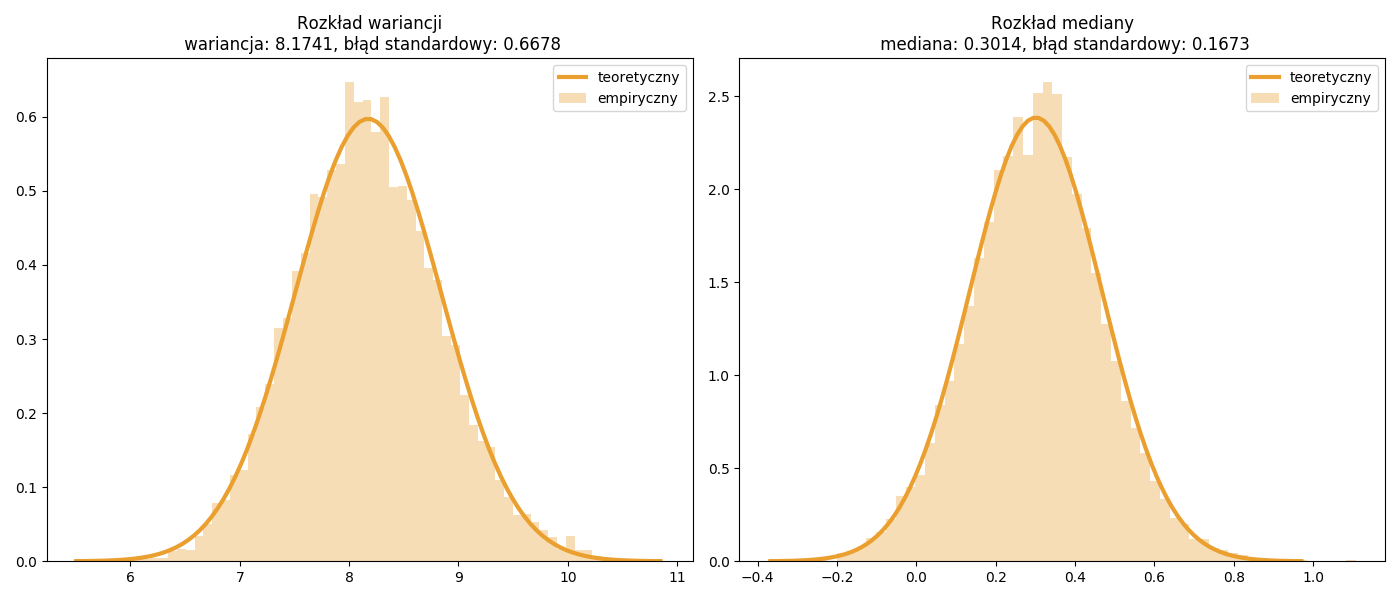
\includegraphics[width=1\linewidth]{boot01} 

}

\caption{Rozkład empiryczny (bootstrap) vs rozkład teoretyczny (normalny).}\label{fig:boot01}
\end{figure}

W metodach symulacyjnych można również wykorzystać generatory liczb losowych jeśli wiemy z jakiego rozkładu pochodzi próba. Przykładowo dla proporcji będzie to rozkład dwumianowy o parametrach np. \(p=0,3\) oraz \(n=50\) (patrz podrozdział \ref{R72}).

\begin{Shaded}
\begin{Highlighting}[]
\ImportTok{import}\NormalTok{ numpy }\ImportTok{as}\NormalTok{ np}
\ImportTok{import}\NormalTok{ scipy.stats }\ImportTok{as}\NormalTok{ stats}

\NormalTok{mc }\OperatorTok{=}\NormalTok{ [np.mean(stats.binom.rvs(n}\OperatorTok{=}\DecValTok{1}\NormalTok{, p}\OperatorTok{=}\FloatTok{0.3}\NormalTok{, loc}\OperatorTok{=}\DecValTok{0}\NormalTok{, size}\OperatorTok{=}\DecValTok{50}\NormalTok{)) }\ControlFlowTok{for}\NormalTok{ i }\KeywordTok{in} \BuiltInTok{range}\NormalTok{(}\DecValTok{10000}\NormalTok{)]}
\NormalTok{P_mc }\OperatorTok{=}\NormalTok{ np.mean(mc)}
\NormalTok{SE_p_mc }\OperatorTok{=}\NormalTok{ np.std(mc,ddof}\OperatorTok{=}\DecValTok{1}\NormalTok{)}
\NormalTok{conf }\OperatorTok{=}\NormalTok{ np.percentile(mc, [}\FloatTok{2.5}\NormalTok{, }\FloatTok{97.5}\NormalTok{])}
\NormalTok{p }\OperatorTok{=}\NormalTok{ np.mean(np.less(mc,[}\FloatTok{0.5}\NormalTok{]))}

\BuiltInTok{print}\NormalTok{(}\StringTok{"proporcja:"}\NormalTok{,P_mc,}\StringTok{", błąd:"}\NormalTok{,SE_p_mc,}\StringTok{"}\CharTok{\textbackslash{}n}\StringTok{95% przedział ufności:"}\NormalTok{,conf)}
\BuiltInTok{print}\NormalTok{(}\StringTok{"}\CharTok{\textbackslash{}n}\StringTok{H0: p = 0.5 vs. H1: p != 0.5"}\NormalTok{,}\StringTok{"}\CharTok{\textbackslash{}n}\StringTok{p-wartość:"}\NormalTok{,}\DecValTok{2}\OperatorTok{*}\BuiltInTok{min}\NormalTok{(p,}\DecValTok{1}\OperatorTok{-}\NormalTok{p))}
\end{Highlighting}
\end{Shaded}

\begin{verbatim}
## proporcja: 0.299728 , błąd: 0.06472607637186306 
## 95% przedział ufności: [0.18 0.42]
## 
## H0: p = 0.5 vs. H1: p != 0.5 
## p-wartość: 0.0027999999999999137
\end{verbatim}

\hypertarget{R8}{%
\chapter{Porównanie zmiennych niezależnych}\label{R8}}

\begin{center}\rule{0.5\linewidth}{\linethickness}\end{center}

\hypertarget{R81}{%
\section{Porównanie średnich}\label{R81}}

\textbf{Test t-Studenta / Test t-Welcha}. Do porównania dwóch średnich tj. do zweryfikowania hipotezy \(H_0:\mu_1=\mu_2\) najczęsciej proponowany jest test t-Studenta Wymaga on spełnienia dwóch warunków: normalność rozkładu oraz jednorodności wariancji. Statystyka klasycznego testu dla dwóch średnich: \((\bar{x}_1-\bar{x}_2)/\sqrt{d_1+d_2}\) ma rozkład t-Studenta ze stopniami swobody \(df=n_1+n_2-2\).
Jeśli wariancje w próbkach nie są równe to zalecane jest stosowanie poprawki Welcha \citep{welch2016} która polega na modyfikacji stopni swobody:
\begin{equation}
df_{\mathrm{Welch}}=\frac{(d_1+d_2)^2}{\frac{d_1}{n_1-1}+\frac{d_2}{n_2-1}}
\label{eq:df01}
\end{equation}
gdzie: \(s_k^2\) to wariancja, \(n_k\) to liczebność próby dla \(k=1,2\) oraz \(d_k=s^2_k/n_k\).

Dzięki funkcji \href{https://pingouin-stats.org/generated/pingouin.ttest.html\#pingouin.ttest}{\texttt{pingouin.ttest}} jest dostępna klasyczna wersja testu t-Studenta oraz z poprawką Welcha.

\begin{Shaded}
\begin{Highlighting}[]
\ImportTok{import}\NormalTok{ scipy.stats }\ImportTok{as}\NormalTok{ stats}
\ImportTok{import}\NormalTok{ pingouin }\ImportTok{as}\NormalTok{ pg}

\NormalTok{x }\OperatorTok{=}\NormalTok{ stats.norm.rvs(}\DecValTok{0}\NormalTok{, }\DecValTok{1}\NormalTok{, size}\OperatorTok{=}\DecValTok{20}\NormalTok{, random_state}\OperatorTok{=}\DecValTok{2305}\NormalTok{)}
\NormalTok{y }\OperatorTok{=}\NormalTok{ stats.norm.rvs(}\FloatTok{1.5}\NormalTok{, }\DecValTok{2}\NormalTok{, size}\OperatorTok{=}\DecValTok{20}\NormalTok{, random_state}\OperatorTok{=}\DecValTok{4101}\NormalTok{)}

\BuiltInTok{print}\NormalTok{(pg.ttest(x,y, correction}\OperatorTok{=}\VariableTok{True}\NormalTok{)[[}\StringTok{'T'}\NormalTok{,}\StringTok{'dof'}\NormalTok{,}\StringTok{'CI95%'}\NormalTok{,}\StringTok{'p-val'}\NormalTok{]])}
\end{Highlighting}
\end{Shaded}

\begin{verbatim}
##             T    dof           CI95%     p-val
## T-test -3.448  23.26  [-2.95, -0.74]  0.002164
\end{verbatim}

\textbf{Anova / Welch-Anova}. Klasyczna analiza wariancji - inaczej ANOVA to rozwinięcie testu t-Studenta dla więcej niż dwóch zmiennych niezależnych. Inaczej mówiąc w przypadku porównania średnich z dwóch grup wyniki z obu procedur są tożsame. Funkcja \href{https://pingouin-stats.org/generated/pingouin.anova.html\#pingouin.anova}{\texttt{pingouin.anova}} realizuje jedno lub dwuczynnikową analizę wariancji z interakcją. Natomiast do funkcji \href{https://pingouin-stats.org/generated/pingouin.welch_anova.html\#pingouin.welch_anova}{\texttt{pingouin.welch\_anova}} jest zaimplementowana metoda Welcha dla jednej zmiennej grupującej.

\begin{Shaded}
\begin{Highlighting}[]
\ImportTok{import}\NormalTok{ numpy }\ImportTok{as}\NormalTok{ np}
\ImportTok{import}\NormalTok{ scipy.stats }\ImportTok{as}\NormalTok{ stats}
\ImportTok{import}\NormalTok{ pandas }\ImportTok{as}\NormalTok{ pd}
\ImportTok{import}\NormalTok{ pingouin }\ImportTok{as}\NormalTok{ pg}

\NormalTok{y }\OperatorTok{=}\NormalTok{ np.concatenate((stats.norm.rvs(}\DecValTok{0}\NormalTok{, }\DecValTok{1}\NormalTok{, size}\OperatorTok{=}\DecValTok{20}\NormalTok{, random_state}\OperatorTok{=}\DecValTok{2305}\NormalTok{),}
\NormalTok{                    stats.norm.rvs(}\FloatTok{1.5}\NormalTok{, }\DecValTok{2}\NormalTok{, size}\OperatorTok{=}\DecValTok{20}\NormalTok{, random_state}\OperatorTok{=}\DecValTok{4101}\NormalTok{),}
\NormalTok{                    stats.norm.rvs(}\FloatTok{1.5}\NormalTok{, }\DecValTok{2}\NormalTok{, size}\OperatorTok{=}\DecValTok{20}\NormalTok{, random_state}\OperatorTok{=}\DecValTok{4026}\NormalTok{)))}
\NormalTok{g }\OperatorTok{=}\NormalTok{ np.repeat(np.linspace(}\DecValTok{1}\NormalTok{,}\DecValTok{3}\NormalTok{,}\DecValTok{3}\NormalTok{), [}\DecValTok{20}\NormalTok{,}\DecValTok{20}\NormalTok{,}\DecValTok{20}\NormalTok{], axis}\OperatorTok{=}\DecValTok{0}\NormalTok{)}

\BuiltInTok{print}\NormalTok{(pg.welch_anova(dv}\OperatorTok{=}\StringTok{'y'}\NormalTok{, between}\OperatorTok{=}\StringTok{'g'}\NormalTok{, data}\OperatorTok{=}\NormalTok{pd.DataFrame(\{}\StringTok{'y'}\NormalTok{:y,}\StringTok{'g'}\NormalTok{:g\})))}
\end{Highlighting}
\end{Shaded}

\begin{verbatim}
##   Source  ddof1   ddof2      F     p-unc
## 0      g      2  30.937  6.448  0.004562
\end{verbatim}

\textbf{Dalsza analiza}. Po odrzuceniu hipotezy zerowej w analizie wariancji stosujemy testy do porównań wielokrotnych. Jednym z bardziej popularnych tzw. testów po fakcie dla grup niezależnych jest procedura Tukeya lub seria testów t-Studenta z odpowiednią korektą p-wartości. Są one zaimplementowane odpowiednio do funkcji
\href{https://pingouin-stats.org/generated/pingouin.pairwise_tukey.html\#pingouin.pairwise_tukey}{\texttt{pingouin.pairwise\_tukey}} oraz \href{https://pingouin-stats.org/generated/pingouin.pairwise_ttests.html\#pingouin.pairwise_ttests}{\texttt{pingouin.pairwise\_ttests}}. Natomiast w warunkach heteroskedastyczności można wykonać serię testów t-Welcha z odpowiednią korektą p-wartości lub test Gamesa-Howella. Są one dostępne odpowiednio w funkcji \href{https://pingouin-stats.org/generated/pingouin.pairwise_ttests.html\#pingouin.pairwise_ttests}{\texttt{pingouin.pairwise\_ttests}} oraz \href{https://pingouin-stats.org/generated/pingouin.pairwise_gameshowell.html\#pingouin.pairwise_gameshowell}{\texttt{pingouin.pairwise\_gameshowell}}. Wiele ciekawych rozwiązań np. test Tamhane T2 zostało zaimplementowanych do pakietu \href{https://scikit-posthocs.readthedocs.io/en/latest/}{\texttt{scikit-posthocs}} który bazuje na bibliotece \href{https://cran.r-project.org/web/packages/PMCMRplus/vignettes/QuickReferenceGuide.html}{\texttt{PMCMRplus}}/\href{https://cran.r-project.org/web/packages/PMCMR/vignettes/PMCMR.pdf}{\texttt{PMCMR}} dla programu R.

\begin{Shaded}
\begin{Highlighting}[]
\ImportTok{import}\NormalTok{ numpy }\ImportTok{as}\NormalTok{ np}
\ImportTok{import}\NormalTok{ scipy.stats }\ImportTok{as}\NormalTok{ stats}
\ImportTok{import}\NormalTok{ pandas }\ImportTok{as}\NormalTok{ pd}
\ImportTok{import}\NormalTok{ pingouin }\ImportTok{as}\NormalTok{ pg}

\NormalTok{y }\OperatorTok{=}\NormalTok{ np.concatenate((stats.norm.rvs(}\DecValTok{0}\NormalTok{, }\DecValTok{1}\NormalTok{, size}\OperatorTok{=}\DecValTok{20}\NormalTok{, random_state}\OperatorTok{=}\DecValTok{2305}\NormalTok{),}
\NormalTok{                    stats.norm.rvs(}\FloatTok{1.5}\NormalTok{, }\DecValTok{2}\NormalTok{, size}\OperatorTok{=}\DecValTok{20}\NormalTok{, random_state}\OperatorTok{=}\DecValTok{4101}\NormalTok{),}
\NormalTok{                    stats.norm.rvs(}\FloatTok{1.5}\NormalTok{, }\DecValTok{2}\NormalTok{, size}\OperatorTok{=}\DecValTok{20}\NormalTok{, random_state}\OperatorTok{=}\DecValTok{4026}\NormalTok{)))}
\NormalTok{g }\OperatorTok{=}\NormalTok{ np.repeat(np.linspace(}\DecValTok{1}\NormalTok{,}\DecValTok{3}\NormalTok{,}\DecValTok{3}\NormalTok{), [}\DecValTok{20}\NormalTok{,}\DecValTok{20}\NormalTok{,}\DecValTok{20}\NormalTok{], axis}\OperatorTok{=}\DecValTok{0}\NormalTok{)}

\BuiltInTok{print}\NormalTok{(pg.pairwise_gameshowell(dv}\OperatorTok{=}\StringTok{'y'}\NormalTok{, between}\OperatorTok{=}\StringTok{'g'}\NormalTok{,}
\NormalTok{                           data}\OperatorTok{=}\NormalTok{pd.DataFrame(\{}\StringTok{'y'}\NormalTok{:y,}\StringTok{'g'}\NormalTok{:g\})))}
\end{Highlighting}
\end{Shaded}

\begin{verbatim}
##      A    B  mean(A)  mean(B)   diff  ...      T      df      pval  efsize  eftype
## 0  1.0  2.0    0.155    2.001 -1.846  ... -3.448  23.261  0.002070  -1.069  hedges
## 1  1.0  3.0    0.155    0.857 -0.702  ... -1.539  25.039  0.275781  -0.477  hedges
## 2  2.0  3.0    2.001    0.857  1.143  ...  1.730  36.818  0.196416   0.536  hedges
## 
## [3 rows x 12 columns]
\end{verbatim}

\hypertarget{R82}{%
\section{Porównanie rang}\label{R82}}

\textbf{Test Manna-Whitneya}. Przy założeniu, że dwa badane rozkłady mają ten sam kształt (takie same wariancje, skośność itp.) można zweryfikować hipotezę zerową o postaci \(H_{0}:\;F(x)=G(y+\Delta)\) w której parametr \(\Delta\) określa przesunięcie dystrybuanty \(G(y)\) względem dystrybuanty \(F(x)\) \citep{med2018}. Inaczej mówiąc rozmieszczenie rozkładów \(F(x)\) i \(G(y)\) różni się w zależności od \(\Delta\). Parametr przesunięcia można oszacować za pomocą estymatorora Hodgesa-Lehmanna:
\begin{equation}
\hat{\Delta}=\mbox{mediana}\{x_i-y_j\;:\;i=1,\;\dots n_1\;;\;j=1,\;\dots n_2\}
\label{eq:mw01}
\end{equation}

Warto zaznaczyć, że parametr \(\Delta\) w funkcji \href{https://docs.scipy.org/doc/scipy/reference/generated/scipy.stats.mannwhitneyu.html\#scipy.stats.mannwhitneyu}{\texttt{scipy.stats.mannwhitneyu}} oraz \href{https://pingouin-stats.org/generated/pingouin.mwu.html\#pingouin.mwu}{\texttt{pingouin.mwu}} ma stałą wartość równą zero. Zatem rozważana hipoteza zerowa ma postać:
\begin{equation}
H_{0}:\;\Delta=0\quad\textrm{vs.}\quad H_{1}:\;\Delta\neq 0
\label{eq:mw02a}
\end{equation}
Równoważnym zapisem może być:
\begin{equation}
H_{0}:\;F(x)=G(y)\quad\textrm{vs.}\quad H_{1}:\;F(x)\neq G(y)
\label{eq:mw02b}
\end{equation}

Statystyka testowa:
\begin{equation}
Z=\frac{|W-\frac{n_1n_2}{2}|-0,5}{\sqrt{\frac{n_1n_2(n_1+n_2+1)}{12}-\frac{n_1n_2\sum_{i=1}^{c}(t^3-t)}{12(n_1+n_2)(n_1+n_2-1)}}}
\label{eq:mw03}
\end{equation}
gdzie: \(c\) to liczba grup pomiarów wiązanych, \(t_i\) to liczba pomiarów wiązanych w \(i\)-tej grupie pomiarów wiązanych.

\begin{Shaded}
\begin{Highlighting}[]
\ImportTok{import}\NormalTok{ scipy.stats }\ImportTok{as}\NormalTok{ stats}
\ImportTok{import}\NormalTok{ pingouin }\ImportTok{as}\NormalTok{ pg}
\ImportTok{import}\NormalTok{ numpy }\ImportTok{as}\NormalTok{ np}

\NormalTok{x }\OperatorTok{=}\NormalTok{ stats.norm.rvs(}\DecValTok{0}\NormalTok{, }\DecValTok{1}\NormalTok{, size}\OperatorTok{=}\DecValTok{20}\NormalTok{, random_state}\OperatorTok{=}\DecValTok{2305}\NormalTok{)}
\NormalTok{y }\OperatorTok{=}\NormalTok{ stats.norm.rvs(}\FloatTok{1.5}\NormalTok{, }\DecValTok{2}\NormalTok{, size}\OperatorTok{=}\DecValTok{20}\NormalTok{, random_state}\OperatorTok{=}\DecValTok{4101}\NormalTok{)}

\NormalTok{hl }\OperatorTok{=}\NormalTok{ np.median(x[:, }\VariableTok{None}\NormalTok{] }\OperatorTok{-}\NormalTok{ y)}
\NormalTok{df }\OperatorTok{=}\NormalTok{ pg.mwu(x,y)}
\NormalTok{df[}\StringTok{'LH-median'}\NormalTok{] }\OperatorTok{=}\NormalTok{ hl}
\BuiltInTok{print}\NormalTok{(df)}
\end{Highlighting}
\end{Shaded}

\begin{verbatim}
##      U-val     p-val   RBC  CLES  LH-median
## MWU   96.0  0.005115  0.52  0.76  -2.003235
\end{verbatim}

\textbf{Test Brunera-Munzela}. Dobrą alternatywną dla testu sumy rang Wilcoxona w warunakch heteroskedastyczności może być test Brunera-Munzela \citep{bm2000} dostępny dzięki funkcji \href{https://docs.scipy.org/doc/scipy/reference/generated/scipy.stats.brunnermunzel.html\#scipy.stats.brunnermunzel}{\texttt{scipy.stats.brunnermunzel}}. Wersja permutacyjna tego testu \citep{neub2007} jest zalecana dla przypadku małolicznych próbek o nierównych liczebnościach. W tym teście
hipoteza zerowa dla równości stochastycznej ma postać:
\begin{equation}
H_0:\;p=0,5\quad\textrm{vs.}\quad H_{1}:\;p\neq 0,5
\label{eq:mw04}
\end{equation}
gdzie \(p\) określa prawdopodobieństwo tego, że obserwacje w grupie pierwszej są zazwyczaj mniejsze niż w grupie drugiej.

Wynika z tego, że prawdopodobieństwo zdarzenia przeciwnego (obserwacje w grupie pierwszej \(x\) są zazwyczaj większe niż w grupie drugiej \(y\)) jest także równe \(0,5\). Zatem w hipotezie zerowej zakładamy, że wartości w obu próbkach mają porównywalne wartości tzn. wartości z pierwszej próbki nie mają tendencji do mniejszych/większych wartości niż w próbce drugiej. Estymację tego prawdopodobieństwa można dokonać w dwojaki sposób:
\begin{equation}
\hat{p}=P(x<y)+0,5\cdot P(x=y)\quad\mbox{lub} \quad \hat{p}=\frac{\bar{r}_2-(n_2+1)\cdot 0,5}{n_1}
\label{eq:mw05}
\end{equation}
gdzie \(\bar{r}_2\) to średnia ranga dla drugiej zmiennej a rangi są liczone na podstawie próbki zbiorczej.

Warto dodać, że na podstawie estymatora prawdopodobieństwa \(\hat{p}\) można obliczyć statystykę testu sumy rang Wilcoxona na podstawie wzoru:
\begin{equation}
W=(1-\hat{p})n_1n_2
\label{eq:mw06}
\end{equation}

Statystyka testu Brunera-Munzela:
\begin{equation}
BM=\frac{n_1n_2(\bar{r}_1-\bar{r}_2)}{(n_1+n_2)\sqrt{n_1s_1^2+n_2s_2^2}}
\label{eq:mw07}
\end{equation}
ma rozkład t-Studenta ze stopniami swobody według formuły:
\begin{equation}
df_{\mathrm{Satterthwaite}}=\frac{(d_1+d_2)^2}{\frac{d_1}{n_1-1}+\frac{d_2}{n_2-1}}
\label{eq:mw08}
\end{equation}
gdzie \(d_k=n_k\cdot s^2_k\) to iloczyn liczebności próby \(n_k\) oraz wariancji \(s_k^2\) dla każdej \(k\)-tej grupy.

Wariancja jest zdefiniowana w następujący sposób:
\begin{equation}
s_k^2=\frac{1}{n_k-1}\sum_{i=1}^{n_k}\left(r_{ki}-w_{ki}-\bar{r}_k+\frac{n_k+1}{2}\right)^2
\label{eq:mw09}
\end{equation}
gdzie: \(\bar{r}_k\) oznacza średnią rangę \(k\)-tej grupy z próbki zbiorczej, \(r_k\) to rangi dla \(k\)-tej grupy z próbki zbiorczej, \(w_k\) to rangi dla \(k\)-tej grupy.

\begin{Shaded}
\begin{Highlighting}[]
\ImportTok{import}\NormalTok{ warnings}
\NormalTok{warnings.filterwarnings(}\StringTok{"ignore"}\NormalTok{)}
\ImportTok{import}\NormalTok{ scipy.stats }\ImportTok{as}\NormalTok{ stats}
\ImportTok{import}\NormalTok{ PyNonpar}
\ImportTok{from}\NormalTok{ PyNonpar }\ImportTok{import} \OperatorTok{*}
    
\NormalTok{x }\OperatorTok{=}\NormalTok{ stats.norm.rvs(}\DecValTok{0}\NormalTok{, }\DecValTok{1}\NormalTok{, size}\OperatorTok{=}\DecValTok{20}\NormalTok{, random_state}\OperatorTok{=}\DecValTok{2305}\NormalTok{).tolist()}
\NormalTok{y }\OperatorTok{=}\NormalTok{ stats.norm.rvs(}\FloatTok{1.5}\NormalTok{, }\DecValTok{2}\NormalTok{, size}\OperatorTok{=}\DecValTok{20}\NormalTok{, random_state}\OperatorTok{=}\DecValTok{4101}\NormalTok{).tolist()}

\NormalTok{res }\OperatorTok{=}\NormalTok{ PyNonpar.twosample.brunner_munzel_test(x,y)}
\BuiltInTok{print}\NormalTok{(}\StringTok{"BM= }\SpecialCharTok{%.4f}\StringTok{, df= }\SpecialCharTok{%.4f}\StringTok{, pvalue= }\SpecialCharTok\NormalTok{ (res[}\DecValTok{1}\NormalTok{],res[}\DecValTok{2}\NormalTok{],res[}\DecValTok{3}\NormalTok{]))}
\end{Highlighting}
\end{Shaded}

\begin{verbatim}
## BM= 2.9380, df= 20.6352, pvalue= 0.0080
\end{verbatim}

\textbf{Test Kruskala-Wallisa}. Nieparametrycznym odpowiednikiem analizy wariancji jest test Kruskala-Walisa jako rozszerzenie testu sumy rang Wilcoxona na kilka grup. W tej metodzie zakładamy, że próbki pochodzą z tego samego rozkładu o dowolnym kształcie. Oznacza to, że rozkład w grupach nie musi być normalny ale w dalszym ciągu zakładamy homoskedastyczność wariancji.
Dokładny rozkład statystyki Kruskala-Wallisa można przybliżać za pomocą metod permutacyjnych lub takich dystrybuant jak: chi-kwadrat, F-Snedecora oraz beta \citep{kw2013}.

Statystyka testowa:
\begin{equation}
\chi^2_{KW}=\left(1-\frac{\sum_{i=1}^{c}(t_i^3-t_i)}{n^3-n}\right)^{-1}\left[\frac{12}{n(n+1)}\left(\sum_{j=1}^{k}\frac{R_j^2}{n_j}\right)-3(n+1)\right]
\label{eq:mw10}
\end{equation}
gdzie: \(n\) to liczebność z wszystkich \(k\) grup, \(n_j\) to liczebność w \(j\)-tej grupie, \(R_j\) to suma rang w \(j\)-tej grupie, \(c\) to liczba grup pomiarów wiązanych, \(t_i\) to liczba pomiarów wiązanych w \(i\)-tej grupie pomiarów wiązanych.

Poniżej implementacja wersji permutacyjnej testu Kruskala-Wallisa:

\begin{Shaded}
\begin{Highlighting}[]
\ImportTok{import}\NormalTok{ numpy }\ImportTok{as}\NormalTok{ np}
\ImportTok{import}\NormalTok{ scipy.stats }\ImportTok{as}\NormalTok{ stats}
\ImportTok{import}\NormalTok{ pandas }\ImportTok{as}\NormalTok{ pd}
\ImportTok{import}\NormalTok{ pingouin }\ImportTok{as}\NormalTok{ pg}

\NormalTok{y }\OperatorTok{=}\NormalTok{ np.concatenate((stats.expon.rvs(}\DecValTok{0}\NormalTok{, }\DecValTok{1}\NormalTok{, size}\OperatorTok{=}\DecValTok{20}\NormalTok{, random_state}\OperatorTok{=}\DecValTok{2305}\NormalTok{),}
\NormalTok{                    stats.expon.rvs(}\FloatTok{0.5}\NormalTok{, }\DecValTok{1}\NormalTok{, size}\OperatorTok{=}\DecValTok{20}\NormalTok{, random_state}\OperatorTok{=}\DecValTok{4101}\NormalTok{),}
\NormalTok{                    stats.expon.rvs(}\DecValTok{1}\NormalTok{, }\DecValTok{1}\NormalTok{, size}\OperatorTok{=}\DecValTok{20}\NormalTok{, random_state}\OperatorTok{=}\DecValTok{4026}\NormalTok{)))}
\NormalTok{g }\OperatorTok{=}\NormalTok{ np.repeat(np.linspace(}\DecValTok{1}\NormalTok{,}\DecValTok{3}\NormalTok{,}\DecValTok{3}\NormalTok{), [}\DecValTok{20}\NormalTok{,}\DecValTok{20}\NormalTok{,}\DecValTok{20}\NormalTok{], axis}\OperatorTok{=}\DecValTok{0}\NormalTok{)}

\NormalTok{kw }\OperatorTok{=}\NormalTok{ pg.kruskal(dv}\OperatorTok{=}\StringTok{'y'}\NormalTok{, between}\OperatorTok{=}\StringTok{'g'}\NormalTok{, data}\OperatorTok{=}\NormalTok{pd.DataFrame(\{}\StringTok{'y'}\NormalTok{:y,}\StringTok{'g'}\NormalTok{:g\}))}

\NormalTok{H }\OperatorTok{=}\NormalTok{ kw[}\StringTok{"H"}\NormalTok{][}\DecValTok{0}\NormalTok{]}
\NormalTok{B }\OperatorTok{=} \DecValTok{1000}
\NormalTok{h }\OperatorTok{=}\NormalTok{ [}\BuiltInTok{list}\NormalTok{(pg.kruskal(dv}\OperatorTok{=}\StringTok{'y'}\NormalTok{, between}\OperatorTok{=}\StringTok{'g'}\NormalTok{,}\OperatorTok{\textbackslash{}}
\NormalTok{          data}\OperatorTok{=}\NormalTok{pd.DataFrame(\{}\StringTok{'y'}\NormalTok{:y,}\StringTok{'g'}\NormalTok{:np.random.choice(g,size}\OperatorTok{=}\DecValTok{60}\NormalTok{)\}))[}\StringTok{"H"}\NormalTok{])[}\DecValTok{0}\NormalTok{]}\OperatorTok{\textbackslash{}}
          \ControlFlowTok{for}\NormalTok{ i }\KeywordTok{in} \BuiltInTok{range}\NormalTok{(B)]}
\NormalTok{perm }\OperatorTok{=}\NormalTok{ np.greater(h,[H]).mean()}
\NormalTok{kw[}\StringTok{"p-perm"}\NormalTok{] }\OperatorTok{=}\NormalTok{ perm}
\BuiltInTok{print}\NormalTok{(kw)}
\end{Highlighting}
\end{Shaded}

\begin{verbatim}
##         Source  ddof1     H     p-unc  p-perm
## Kruskal      g      2  7.61  0.022254   0.017
\end{verbatim}

\textbf{ANOVA-rank}. Warto zauważyć, że problem heterogeniczności wariancji można uwzględnić za pomocą testu Brunner-Dette-Munk \citep{BDM1997} w którym można także testować interakcję w dwuczynnikowej analizie wariancji. Jednak ta metoda nie jest dostępna w pakietach \href{https://docs.scipy.org/doc/scipy/reference/stats.html}{\texttt{scipy.stats}} oraz \href{https://pingouin-stats.org/index.html}{\texttt{pingouin}}. Alternatywą może być zastosowanie procedury wykorzystującej rozkład F-Snedecora która polega na porangowaniu danych i zastosowaniu klasycznej metody ANOVA. Innym rozwiązaniem może być wykorzystanie ważonej metody najmniejszych kwadratów lub odpornych błędów standardowych z wykorzystaniem funkcji \href{https://www.statsmodels.org/stable/generated/statsmodels.stats.anova.anova_lm.html\#statsmodels.stats.anova.anova_lm}{\texttt{statsmodels.stats.anova.anova\_lm}}.

\begin{Shaded}
\begin{Highlighting}[]
\ImportTok{import}\NormalTok{ numpy }\ImportTok{as}\NormalTok{ np}
\ImportTok{import}\NormalTok{ scipy.stats }\ImportTok{as}\NormalTok{ stats}
\ImportTok{import}\NormalTok{ pandas }\ImportTok{as}\NormalTok{ pd}
\ImportTok{import}\NormalTok{ pingouin }\ImportTok{as}\NormalTok{ pg}

\NormalTok{y }\OperatorTok{=}\NormalTok{ np.concatenate((stats.expon.rvs(}\DecValTok{0}\NormalTok{, }\DecValTok{1}\NormalTok{, size}\OperatorTok{=}\DecValTok{20}\NormalTok{, random_state}\OperatorTok{=}\DecValTok{2305}\NormalTok{),}
\NormalTok{                    stats.expon.rvs(}\FloatTok{0.5}\NormalTok{, }\DecValTok{1}\NormalTok{, size}\OperatorTok{=}\DecValTok{20}\NormalTok{, random_state}\OperatorTok{=}\DecValTok{4101}\NormalTok{),}
\NormalTok{                    stats.expon.rvs(}\DecValTok{1}\NormalTok{, }\DecValTok{1}\NormalTok{, size}\OperatorTok{=}\DecValTok{20}\NormalTok{, random_state}\OperatorTok{=}\DecValTok{4026}\NormalTok{)))}
\NormalTok{r }\OperatorTok{=}\NormalTok{ stats.rankdata(y)}
\NormalTok{g }\OperatorTok{=}\NormalTok{ np.repeat(np.linspace(}\DecValTok{1}\NormalTok{,}\DecValTok{3}\NormalTok{,}\DecValTok{3}\NormalTok{), [}\DecValTok{20}\NormalTok{,}\DecValTok{20}\NormalTok{,}\DecValTok{20}\NormalTok{], axis}\OperatorTok{=}\DecValTok{0}\NormalTok{)}
\NormalTok{d }\OperatorTok{=}\NormalTok{ pd.DataFrame(\{}\StringTok{"y"}\NormalTok{:y,}\StringTok{"g"}\NormalTok{:g,}\StringTok{"r"}\NormalTok{:r\})}
\BuiltInTok{print}\NormalTok{(pg.anova(dv}\OperatorTok{=}\StringTok{'r'}\NormalTok{, between}\OperatorTok{=}\StringTok{'g'}\NormalTok{, data}\OperatorTok{=}\NormalTok{d))}
\end{Highlighting}
\end{Shaded}

\begin{verbatim}
##   Source  ddof1  ddof2      F     p-unc    np2
## 0      g      2     57  4.221  0.019527  0.129
\end{verbatim}

\textbf{Dalsza analiza}. Po odrzuceniu hipotezy zerowej w teście Kruskala-Wallisa można dokonać bardziej szczególowej analizy czyli przeprowadzić porównania wielokrotne. Popularnym rozwiązaniem jest zastosowanie serii testów sumy rang Wilcoxona. Ta metoda jest dostępna dzięki funkcji \href{https://pingouin-stats.org/generated/pingouin.pairwise_ttests.html\#pingouin.pairwise_ttests}{\texttt{pingouin.pairwise\_ttests}} z zaznaczeniem opcji \texttt{parametric=False}. Jednak szerszy zestaw testów post hoc dla grup niezależnych znajdziemy w pakiecie \href{https://scikit-posthocs.readthedocs.io/en/latest/intro/}{\texttt{scikit-posthocs}}. Poniżej przykład testu Conovera.

\begin{Shaded}
\begin{Highlighting}[]
\ImportTok{import}\NormalTok{ numpy }\ImportTok{as}\NormalTok{ np}
\ImportTok{import}\NormalTok{ scipy.stats }\ImportTok{as}\NormalTok{ stats}
\ImportTok{import}\NormalTok{ pandas }\ImportTok{as}\NormalTok{ pd}
\ImportTok{import}\NormalTok{ pingouin }\ImportTok{as}\NormalTok{ pg}
\ImportTok{from}\NormalTok{ scikit_posthocs }\ImportTok{import}\NormalTok{ posthoc_conover}

\NormalTok{y }\OperatorTok{=}\NormalTok{ np.concatenate((stats.expon.rvs(}\DecValTok{0}\NormalTok{, }\DecValTok{1}\NormalTok{, size}\OperatorTok{=}\DecValTok{20}\NormalTok{, random_state}\OperatorTok{=}\DecValTok{2305}\NormalTok{),}
\NormalTok{                    stats.expon.rvs(}\FloatTok{0.5}\NormalTok{, }\DecValTok{1}\NormalTok{, size}\OperatorTok{=}\DecValTok{20}\NormalTok{, random_state}\OperatorTok{=}\DecValTok{4101}\NormalTok{),}
\NormalTok{                    stats.expon.rvs(}\DecValTok{1}\NormalTok{, }\DecValTok{1}\NormalTok{, size}\OperatorTok{=}\DecValTok{20}\NormalTok{, random_state}\OperatorTok{=}\DecValTok{4026}\NormalTok{)))}
\NormalTok{r }\OperatorTok{=}\NormalTok{ stats.rankdata(y)}
\NormalTok{g }\OperatorTok{=}\NormalTok{ np.repeat(np.linspace(}\DecValTok{1}\NormalTok{,}\DecValTok{3}\NormalTok{,}\DecValTok{3}\NormalTok{), [}\DecValTok{20}\NormalTok{,}\DecValTok{20}\NormalTok{,}\DecValTok{20}\NormalTok{], axis}\OperatorTok{=}\DecValTok{0}\NormalTok{)}
\NormalTok{d }\OperatorTok{=}\NormalTok{ pd.DataFrame(\{}\StringTok{"y"}\NormalTok{:y,}\StringTok{"g"}\NormalTok{:g,}\StringTok{"r"}\NormalTok{:r\})}
\BuiltInTok{print}\NormalTok{(posthoc_conover(d, val_col}\OperatorTok{=}\StringTok{'y'}\NormalTok{, group_col}\OperatorTok{=}\StringTok{'g'}\NormalTok{, p_adjust}\OperatorTok{=}\StringTok{'holm'}\NormalTok{))}
\end{Highlighting}
\end{Shaded}

\begin{verbatim}
##           1.0       2.0       3.0
## 1.0 -1.000000  0.221096  0.015936
## 2.0  0.221096 -1.000000  0.221096
## 3.0  0.015936  0.221096 -1.000000
\end{verbatim}

\hypertarget{R83}{%
\section{Porównanie wariancji}\label{R83}}

\textbf{Test Z-diff / Test Z-ratio}. Jeśli chcemy porównać dwie wariancje to rozważamy hipotezy statystyczne o postaci:
\begin{equation}
H_0:\;\sigma_1^2=\sigma_2^2\quad\mbox{vs.}\quad H_1:\;\sigma_1^2\neq\sigma_2^2
\label{eq:v01}
\end{equation}
Zauważmy, że powyższą hipotezę statystyczną można sprowadzić do zapisu:
\begin{equation}
H_{0}:\;\sigma^2_1/\sigma^2_2=1\quad\textrm{vs.}\quad H_{1}:\;\sigma^2_1/\sigma^2_2\neq1
\label{eq:v02}
\end{equation}
Statystyka testowa:
\begin{equation}
Z_{ratio}=\frac{(s^2_1/s^2_2)-1}{SE_{ratio}}
\label{eq:v03}
\end{equation}
gdzie: \(SE_{ratio}=\frac{1}{s_2^{2}}\sqrt{SE_1^2+r_0^2\cdot SE_2^2}\) to błąd standardowy ilorazu dwóch wariancji oraz \(SE=\sqrt{s^2/n}\) to błąd standardowy wariancji \(s^2\) dla przekształconej zmiennej \((x_i-\bar{x})^2\), \(r_0^2\) to iloraz wariancji podniesiony do drugiej potęgi.

\begin{Shaded}
\begin{Highlighting}[]
\ImportTok{import}\NormalTok{ scipy.stats }\ImportTok{as}\NormalTok{ stats}
\ImportTok{import}\NormalTok{ numpy }\ImportTok{as}\NormalTok{ np}

\NormalTok{x }\OperatorTok{=}\NormalTok{ stats.norm.rvs(}\DecValTok{0}\NormalTok{, }\FloatTok{1.5}\NormalTok{, size}\OperatorTok{=}\DecValTok{20}\NormalTok{, random_state}\OperatorTok{=}\DecValTok{2305}\NormalTok{)}
\NormalTok{y }\OperatorTok{=}\NormalTok{ stats.norm.rvs(}\FloatTok{1.5}\NormalTok{, }\DecValTok{2}\NormalTok{, size}\OperatorTok{=}\DecValTok{20}\NormalTok{, random_state}\OperatorTok{=}\DecValTok{4101}\NormalTok{)}
  
\NormalTok{z1 }\OperatorTok{=}\NormalTok{ (x}\OperatorTok{-}\NormalTok{np.mean(x))}\OperatorTok{**}\DecValTok{2}
\NormalTok{z2 }\OperatorTok{=}\NormalTok{ (y}\OperatorTok{-}\NormalTok{np.mean(y))}\OperatorTok{**}\DecValTok{2}
\NormalTok{ratV }\OperatorTok{=}\NormalTok{ np.var(x,ddof}\OperatorTok{=}\DecValTok{1}\NormalTok{)}\OperatorTok{/}\NormalTok{np.var(y,ddof}\OperatorTok{=}\DecValTok{1}\NormalTok{)}
\NormalTok{SE }\OperatorTok{=}\NormalTok{ np.sqrt(np.var(z1,ddof}\OperatorTok{=}\DecValTok{1}\NormalTok{)}\OperatorTok{/}\BuiltInTok{len}\NormalTok{(x)}\OperatorTok{+}\NormalTok{ratV}\OperatorTok{**}\DecValTok{2}\OperatorTok{*}\NormalTok{np.var(z2,ddof}\OperatorTok{=}\DecValTok{1}\NormalTok{)}\OperatorTok{/}\BuiltInTok{len}\NormalTok{(y))}\OperatorTok{/}\NormalTok{np.var(y,ddof}\OperatorTok{=}\DecValTok{1}\NormalTok{)}
\NormalTok{conf }\OperatorTok{=}\NormalTok{ [stats.norm.ppf(i,ratV,SE) }\ControlFlowTok{for}\NormalTok{ i }\KeywordTok{in}\NormalTok{ [}\FloatTok{0.025}\NormalTok{,}\FloatTok{0.975}\NormalTok{]]}
\NormalTok{h0 }\OperatorTok{=} \DecValTok{1}
\NormalTok{p }\OperatorTok{=}\NormalTok{ stats.norm.cdf(h0,ratV,SE)}

\BuiltInTok{print}\NormalTok{(}\StringTok{"iloraz wariancji:"}\NormalTok{,ratV,}\StringTok{", błąd:"}\NormalTok{,SE)}
\BuiltInTok{print}\NormalTok{(}\StringTok{"95% przedział ufności:"}\NormalTok{,conf)}
\BuiltInTok{print}\NormalTok{(}\StringTok{"}\CharTok{\textbackslash{}n}\StringTok{H0: rVar = %.0f vs. H1: rVar != %.0f"} \OperatorTok{%}\NormalTok{ (h0,h0))}
\BuiltInTok{print}\NormalTok{(}\StringTok{"p-wartość:"}\NormalTok{,}\DecValTok{2}\OperatorTok{*}\BuiltInTok{min}\NormalTok{(p,}\DecValTok{1}\OperatorTok{-}\NormalTok{p))}
\end{Highlighting}
\end{Shaded}

\begin{verbatim}
## iloraz wariancji: 0.2555508988591833 , błąd: 0.0975515172257403
## 95% przedział ufności: [0.06435343845949357, 0.446748359258873]
## 
## H0: rVar = 1 vs. H1: rVar != 1
## p-wartość: 2.3314683517128287e-14
\end{verbatim}

Równoważnym zapisem powyższych hipotez statystycznych \eqref{eq:v01} oraz \eqref{eq:v02} będzie zapis:
\begin{equation}
H_{0}:\;\sigma^2_1-\sigma^2_2=0\quad\textrm{vs.}\quad H_{1}:\;\sigma^2_1-\sigma^2_2\neq0
\label{eq:v04}
\end{equation}
Statystyka testowa:
\begin{equation}
Z_{diff}=\frac{(s^2_1-s^2_2)-0}{SE_{diff}}
\label{eq:v05}
\end{equation}

gdzie: \(SE_{diff}=\sqrt{SE_{1}^2+\rho^2\cdot SE_{2}^2}\) to błąd standardowy różnicy dwóch wariancji oraz \(SE=\sqrt{s^2/n}\) to błąd standardowy wariancji \(s^2\) dla przekształconej zmiennej \((x_i-\bar{x})^2\), \(\rho^2\) to opcjonalny parametr do osłabienia/wzmocnienia udziału drugiej wariancji.

\begin{Shaded}
\begin{Highlighting}[]
\ImportTok{import}\NormalTok{ scipy.stats }\ImportTok{as}\NormalTok{ stats}
\ImportTok{import}\NormalTok{ numpy }\ImportTok{as}\NormalTok{ np}

\NormalTok{x }\OperatorTok{=}\NormalTok{ stats.norm.rvs(}\DecValTok{0}\NormalTok{, }\FloatTok{1.5}\NormalTok{, size}\OperatorTok{=}\DecValTok{20}\NormalTok{, random_state}\OperatorTok{=}\DecValTok{2305}\NormalTok{)}
\NormalTok{y }\OperatorTok{=}\NormalTok{ stats.norm.rvs(}\FloatTok{1.5}\NormalTok{, }\DecValTok{2}\NormalTok{, size}\OperatorTok{=}\DecValTok{20}\NormalTok{, random_state}\OperatorTok{=}\DecValTok{4101}\NormalTok{)}

\NormalTok{z1 }\OperatorTok{=}\NormalTok{ (x}\OperatorTok{-}\NormalTok{np.mean(x))}\OperatorTok{**}\DecValTok{2}
\NormalTok{z2 }\OperatorTok{=}\NormalTok{ (y}\OperatorTok{-}\NormalTok{np.mean(y))}\OperatorTok{**}\DecValTok{2}
\NormalTok{difV }\OperatorTok{=}\NormalTok{ np.var(x,ddof}\OperatorTok{=}\DecValTok{1}\NormalTok{)}\OperatorTok{-}\NormalTok{np.var(y,ddof}\OperatorTok{=}\DecValTok{1}\NormalTok{)}
\NormalTok{SE }\OperatorTok{=}\NormalTok{ np.sqrt(np.var(z1,ddof}\OperatorTok{=}\DecValTok{1}\NormalTok{)}\OperatorTok{/}\BuiltInTok{len}\NormalTok{(x)}\OperatorTok{+}\DecValTok{1}\OperatorTok{*}\NormalTok{np.var(z2,ddof}\OperatorTok{=}\DecValTok{1}\NormalTok{)}\OperatorTok{/}\BuiltInTok{len}\NormalTok{(y))}
\NormalTok{conf }\OperatorTok{=}\NormalTok{ [stats.norm.ppf(i,difV,SE) }\ControlFlowTok{for}\NormalTok{ i }\KeywordTok{in}\NormalTok{ [}\FloatTok{0.025}\NormalTok{,}\FloatTok{0.975}\NormalTok{]]}
\NormalTok{h0 }\OperatorTok{=} \DecValTok{0}
\NormalTok{p }\OperatorTok{=}\NormalTok{ stats.norm.cdf(h0,difV,SE)}

\BuiltInTok{print}\NormalTok{(}\StringTok{"różnica wariancji:"}\NormalTok{,difV,}\StringTok{", błąd:"}\NormalTok{,SE)}
\BuiltInTok{print}\NormalTok{(}\StringTok{"95% przedział ufności:"}\NormalTok{,conf)}
\BuiltInTok{print}\NormalTok{(}\StringTok{"}\CharTok{\textbackslash{}n}\StringTok{H0: dVar = %.0f vs. H1: dVar != %.0f"} \OperatorTok{%}\NormalTok{ (h0,h0))}
\BuiltInTok{print}\NormalTok{(}\StringTok{"p-wartość:"}\NormalTok{,}\DecValTok{2}\OperatorTok{*}\BuiltInTok{min}\NormalTok{(p,}\DecValTok{1}\OperatorTok{-}\NormalTok{p))}
\end{Highlighting}
\end{Shaded}

\begin{verbatim}
## różnica wariancji: -3.8307446353496024 , błąd: 1.267036271883883
## 95% przedział ufności: [-6.314090095347914, -1.347399175351292]
## 
## H0: dVar = 0 vs. H1: dVar != 0
## p-wartość: 0.0024995998590693347
\end{verbatim}

\textbf{Test Bartletta / Test Levene}. Badanie równości wariancji można wykonać również za pomocą testu Fligner-Killen lub testu Levene które w przeciwieństwie do testu Bartletta są mało wrażliwe na odchylenia od rozkładu normalnego w próbkach. Przeważnie są one stosowane do badania równości kilku wariancji ale nic nie stoi na przeszkodzie aby wykorzystać je do porównania dwóch wariancji na podstawie hipotezy \eqref{eq:v01}. Dodajmy, że test Levene i Fligner-Killeen mogą występować w trzech wariantach tzn. za parametr lokalizacji można przyjąć średnią, średnią uciętą lub medianę. Taki wybór oferują funkcje \href{https://docs.scipy.org/doc/scipy/reference/generated/scipy.stats.levene.html\#scipy.stats.levene}{\texttt{scipy.stats.levene}} oraz \href{https://docs.scipy.org/doc/scipy/reference/generated/scipy.stats.fligner.html\#scipy.stats.fligner}{\texttt{scipy.stats.fligner}}. Natomiast funkcja \href{https://pingouin-stats.org/generated/pingouin.homoscedasticity.html\#pingouin.homoscedasticity}{\texttt{pingouin.homoscedasticity}} jako parametr lokalizacji stosuje medianę. Jeśli zmienne mają rozkład normalny to podawany jest wynik testu Bartletta.

\begin{Shaded}
\begin{Highlighting}[]
\ImportTok{import}\NormalTok{ scipy.stats }\ImportTok{as}\NormalTok{ stats}
\ImportTok{import}\NormalTok{ numpy }\ImportTok{as}\NormalTok{ np}
\ImportTok{import}\NormalTok{ pingouin }\ImportTok{as}\NormalTok{ pg}

\NormalTok{x }\OperatorTok{=}\NormalTok{ stats.norm.rvs(}\DecValTok{0}\NormalTok{, }\FloatTok{1.5}\NormalTok{, size}\OperatorTok{=}\DecValTok{20}\NormalTok{, random_state}\OperatorTok{=}\DecValTok{2305}\NormalTok{)}
\NormalTok{y }\OperatorTok{=}\NormalTok{ stats.norm.rvs(}\FloatTok{1.5}\NormalTok{, }\DecValTok{2}\NormalTok{, size}\OperatorTok{=}\DecValTok{20}\NormalTok{, random_state}\OperatorTok{=}\DecValTok{4101}\NormalTok{)}

\BuiltInTok{print}\NormalTok{(stats.levene(x,y))}
\BuiltInTok{print}\NormalTok{(stats.fligner(x,y))}
\BuiltInTok{print}\NormalTok{(stats.bartlett(x,y))}
\BuiltInTok{print}\NormalTok{(pg.homoscedasticity(x,y))}
\end{Highlighting}
\end{Shaded}

\begin{verbatim}
## LeveneResult(statistic=8.994663638939507, pvalue=0.0047575161444811925)
## FlignerResult(statistic=6.954492770953616, pvalue=0.008360900023288296)
## BartlettResult(statistic=8.019535289470467, pvalue=0.004627544281207727)
## (False, 0.005)
\end{verbatim}

\hypertarget{R84}{%
\section{Porównanie rozkładów}\label{R84}}

\textbf{Test normalności Andersona-Darlinga}. Założenie normalności zmiennych to jedno z głównych założeń w klasycznej statystyce. W związku z tym zostało opracowanych wiele metod porównywania dystrybuanty empirycznej z rozkładem normalnym. Jednym z bardziej popularnych rozwiązań jest test Shapiro-Wilka który wymaga aby liczebność próby nie przekraczała 5000 elementów. Inne metody jak np. test Jarque-Bera, D'Agostino-Pearsona czy Andersona-Darlinga nie mają tego ograniczenia. Dodajmy jeszcze, że wysoka moc testu może być dobrym uzasadnieniem wyboru konkretnej metody \citep{biecek2013}. Przykładowo test normalności Andersona-Darlinga może być ciekawą alternatywą dla testu Shapiro-Wilka w przypadku wielomodalności lub występowania grubych ogonów \citep[str. 244-246]{biecek2017}.

Statystyka testu Andersona-Darlinga ma postać:
\begin{equation}
AD = -n-\frac{1}{n}\sum_{i=1}^n(2i-1)\big(\ln(z_i)+\ln(1-z_{n+1-i})\big)
\label{eq:v06}
\end{equation}
gdzie: \(z_i\) to wartości wyznaczone na podstawie dystrybuanty rozkładu normalnego \(\Phi(x_i,\bar{x},s)\) dla posortowanych rosnąco elementów próby \(x_i\).

W przypadku badania normalności o nieznanych parametrach \(\mu\) oraz \(\sigma\) jest stosowana poprawka:
\begin{equation}
A1=AD\left(1+\frac{0,75}{n}+\frac{2,25}{n^2}\right)
\label{eq:v07}
\end{equation}

Weryfikację hipotezy zerowej można wykonać w oparciu o otrzymaną p-wartość która jest uzależniona od wartości statystyki testu \eqref{eq:v07}.

\begin{itemize}
\tightlist
\item
  jeżeli \(A1 < 0,2\) to:
\end{itemize}

\begin{equation}
p-value=1-\exp(-13,436+101,14\,A1-223,73\,A1^2)
\label{eq:v08a}
\end{equation}

\begin{itemize}
\tightlist
\item
  jeżeli \(0,2\leq A1<0,34\) to:
\end{itemize}

\begin{equation}
p-value=1-\exp(-8,318+42,796\,A1-59,938\,A1^2)
\label{eq:v08b}
\end{equation}

\begin{itemize}
\tightlist
\item
  jeżeli \(0,34\leq A1 < 0,6\) to:
\end{itemize}

\begin{equation}
p-value=\exp(0,9177-4,279\,A1-1,38\,A1^2)
\label{eq:v08c}
\end{equation}

\begin{itemize}
\tightlist
\item
  jeżeli \(A1\geq 0,6\) to:
\end{itemize}

\begin{equation}
p-value= \exp(1,2937-5,709\,A1+0,0186\,A1^2)
\label{eq:v08d}
\end{equation}

\begin{Shaded}
\begin{Highlighting}[]
\ImportTok{import}\NormalTok{ scipy.stats }\ImportTok{as}\NormalTok{ stats}
\ImportTok{from}\NormalTok{ statsmodels.stats.diagnostic }\ImportTok{import}\NormalTok{ normal_ad}
  
\NormalTok{x }\OperatorTok{=}\NormalTok{ stats.norm.rvs(}\DecValTok{0}\NormalTok{, }\FloatTok{1.5}\NormalTok{, size}\OperatorTok{=}\DecValTok{20}\NormalTok{, random_state}\OperatorTok{=}\DecValTok{2305}\NormalTok{)}
\NormalTok{ad }\OperatorTok{=}\NormalTok{ normal_ad(x)}
\BuiltInTok{print}\NormalTok{(}\StringTok{'AD = }\SpecialCharTok{%.4f}\StringTok{, p-value = }\SpecialCharTok\NormalTok{ (ad[}\DecValTok{0}\NormalTok{],ad[}\DecValTok{1}\NormalTok{]))}
\end{Highlighting}
\end{Shaded}

\begin{verbatim}
## AD = 0.2568, p-value = 0.6848
\end{verbatim}

W stosunkowo prosty sposób można wygenerować wartości krytyczne na podstawie wzoru:

\begin{equation}
A_{crit}=a\left(1-\frac{b}{n}-\frac{d}{n^2}\right)
\label{eq:v09}
\end{equation}
gdzie \(n\) to liczebności próby oraz \(a\), \(b\) i \(d\) to parametry które zależą od poziomu istotności \(\alpha\):
\begin{equation}
\begin{array}{c|llllll}
  \alpha & 0.005 & 0.01 & 0.025 & 0.05 & 0.10 & 0.20\\
  \hline\hline
  a & 1.1578 & 1.0348 & 0.8728 & 0.7514 & 0.6305 & 0.5091\\
  b & 1.063 & 1.013 & 0.881 & 0.795 & 0.750 & 0.756\\
  d & 1.34 & 0.93 & 0.94 & 0.89 & 0.80 & 0.39
 \end{array}
\label{eq:v10}
\end{equation}
Poniżej przykład wygenerowania różnych wartości krytycznych testu normalności Andersona-Darlinga.

\begin{Shaded}
\begin{Highlighting}[]
\ImportTok{import}\NormalTok{ numpy }\ImportTok{as}\NormalTok{ np}
\ImportTok{import}\NormalTok{ scipy.stats }\ImportTok{as}\NormalTok{ stats}
\ImportTok{import}\NormalTok{ pandas }\ImportTok{as}\NormalTok{ pd}

\KeywordTok{def}\NormalTok{ q(alpha}\OperatorTok{=}\FloatTok{0.05}\NormalTok{,n}\OperatorTok{=}\DecValTok{10}\NormalTok{):}
    \ControlFlowTok{if}\NormalTok{ alpha }\OperatorTok{==} \FloatTok{0.005}\NormalTok{:}\OperatorTok{\textbackslash{}}
    \ControlFlowTok{return} \FloatTok{1.1578}\OperatorTok{*}\NormalTok{(}\DecValTok{1}\FloatTok{-1.063}\OperatorTok{/}\NormalTok{n}\FloatTok{-1.34}\OperatorTok{/}\NormalTok{n}\OperatorTok{**}\DecValTok{2}\NormalTok{)}
    \ControlFlowTok{elif}\NormalTok{ alpha }\OperatorTok{==} \FloatTok{0.01}\NormalTok{:}\OperatorTok{\textbackslash{}}
    \ControlFlowTok{return} \FloatTok{1.0348}\OperatorTok{*}\NormalTok{(}\DecValTok{1}\FloatTok{-1.013}\OperatorTok{/}\NormalTok{n}\FloatTok{-0.93}\OperatorTok{/}\NormalTok{n}\OperatorTok{**}\DecValTok{2}\NormalTok{)}
    \ControlFlowTok{elif}\NormalTok{ alpha }\OperatorTok{==} \FloatTok{0.025}\NormalTok{:}\OperatorTok{\textbackslash{}}
    \ControlFlowTok{return} \FloatTok{0.8728}\OperatorTok{*}\NormalTok{(}\DecValTok{1}\FloatTok{-0.881}\OperatorTok{/}\NormalTok{n}\FloatTok{-0.94}\OperatorTok{/}\NormalTok{n}\OperatorTok{**}\DecValTok{2}\NormalTok{)}
    \ControlFlowTok{elif}\NormalTok{ alpha}\OperatorTok{==}\FloatTok{0.05}\NormalTok{:}\OperatorTok{\textbackslash{}}
    \ControlFlowTok{return} \FloatTok{0.7514}\OperatorTok{*}\NormalTok{(}\DecValTok{1}\FloatTok{-0.795}\OperatorTok{/}\NormalTok{n}\FloatTok{-0.89}\OperatorTok{/}\NormalTok{n}\OperatorTok{**}\DecValTok{2}\NormalTok{)}
    \ControlFlowTok{elif}\NormalTok{ alpha }\OperatorTok{==} \FloatTok{0.1}\NormalTok{:}\OperatorTok{\textbackslash{}}
    \ControlFlowTok{return} \FloatTok{0.6305}\OperatorTok{*}\NormalTok{(}\DecValTok{1}\FloatTok{-0.750}\OperatorTok{/}\NormalTok{n}\FloatTok{-0.80}\OperatorTok{/}\NormalTok{n}\OperatorTok{**}\DecValTok{2}\NormalTok{)}
    \ControlFlowTok{elif}\NormalTok{ alpha }\OperatorTok{==} \FloatTok{0.2}\NormalTok{:}\OperatorTok{\textbackslash{}}
    \ControlFlowTok{return} \FloatTok{0.5091}\OperatorTok{*}\NormalTok{(}\DecValTok{1}\FloatTok{-0.756}\OperatorTok{/}\NormalTok{n}\FloatTok{-0.39}\OperatorTok{/}\NormalTok{n}\OperatorTok{**}\DecValTok{2}\NormalTok{)}

\NormalTok{n }\OperatorTok{=}\NormalTok{ [}\DecValTok{20}\NormalTok{,}\DecValTok{50}\NormalTok{,}\DecValTok{100}\NormalTok{,}\DecValTok{150}\NormalTok{,}\DecValTok{300}\NormalTok{,}\DecValTok{900}\NormalTok{,}\DecValTok{1500}\NormalTok{]}
\NormalTok{q0_01  }\OperatorTok{=}\NormalTok{ [q(alpha}\OperatorTok{=}\FloatTok{0.01}\NormalTok{, n}\OperatorTok{=}\NormalTok{i) }\ControlFlowTok{for}\NormalTok{ i }\KeywordTok{in}\NormalTok{ n]}
\NormalTok{q0_025 }\OperatorTok{=}\NormalTok{ [q(alpha}\OperatorTok{=}\FloatTok{0.025}\NormalTok{,n}\OperatorTok{=}\NormalTok{i) }\ControlFlowTok{for}\NormalTok{ i }\KeywordTok{in}\NormalTok{ n]}
\NormalTok{q0_05  }\OperatorTok{=}\NormalTok{ [q(alpha}\OperatorTok{=}\FloatTok{0.05}\NormalTok{, n}\OperatorTok{=}\NormalTok{i) }\ControlFlowTok{for}\NormalTok{ i }\KeywordTok{in}\NormalTok{ n]}
\NormalTok{q0_1   }\OperatorTok{=}\NormalTok{ [q(alpha}\OperatorTok{=}\FloatTok{0.1}\NormalTok{,  n}\OperatorTok{=}\NormalTok{i) }\ControlFlowTok{for}\NormalTok{ i }\KeywordTok{in}\NormalTok{ n]}
\BuiltInTok{print}\NormalTok{(pd.DataFrame(\{}\StringTok{'1%'}\NormalTok{:q0_01,}\StringTok{'2.5%'}\NormalTok{:q0_025,}\StringTok{'5%'}\NormalTok{:q0_05,}\StringTok{'10%'}\NormalTok{:q0_1\},index}\OperatorTok{=}\NormalTok{n))}
\end{Highlighting}
\end{Shaded}

\begin{verbatim}
##             1%      2.5%        5%       10%
## 20    0.979981  0.832302  0.719860  0.605595
## 50    1.013450  0.857093  0.739185  0.620841
## 100   1.024221  0.865029  0.745359  0.625721
## 150   1.027769  0.867637  0.747388  0.627325
## 300   1.031295  0.870228  0.749401  0.628918
## 900   1.033634  0.871945  0.750735  0.629974
## 1500  1.034101  0.872287  0.751001  0.630185
\end{verbatim}

Poniżej wygenerujemy w sposób symulacyjny wartości krytyczne dla \(n=20\):

\begin{Shaded}
\begin{Highlighting}[]
\ImportTok{from}\NormalTok{ statsmodels.stats.diagnostic }\ImportTok{import}\NormalTok{ normal_ad}
\ImportTok{import}\NormalTok{ numpy }\ImportTok{as}\NormalTok{ np}
\ImportTok{import}\NormalTok{ scipy.stats }\ImportTok{as}\NormalTok{ stats}
\ImportTok{import}\NormalTok{ pandas }\ImportTok{as}\NormalTok{ pd}
  
\NormalTok{res }\OperatorTok{=}\NormalTok{ [normal_ad(stats.norm.rvs(}\DecValTok{0}\NormalTok{, }\FloatTok{1.5}\NormalTok{, size}\OperatorTok{=}\DecValTok{20}\NormalTok{))[}\DecValTok{0}\NormalTok{] }\ControlFlowTok{for}\NormalTok{ i }\KeywordTok{in} \BuiltInTok{range}\NormalTok{(}\DecValTok{10000}\NormalTok{)]}
\NormalTok{q }\OperatorTok{=}\NormalTok{ np.percentile(res,[}\DecValTok{99}\NormalTok{,}\FloatTok{97.5}\NormalTok{,}\DecValTok{95}\NormalTok{,}\DecValTok{90}\NormalTok{])}
\BuiltInTok{print}\NormalTok{(pd.DataFrame(\{}\StringTok{'1%'}\NormalTok{:q[}\DecValTok{0}\NormalTok{],}\StringTok{'2.5%'}\NormalTok{:q[}\DecValTok{1}\NormalTok{],}\StringTok{'5%'}\NormalTok{:q[}\DecValTok{2}\NormalTok{],}\StringTok{'10%'}\NormalTok{:q[}\DecValTok{3}\NormalTok{]\},index}\OperatorTok{=}\NormalTok{[}\StringTok{'20'}\NormalTok{]))}
\end{Highlighting}
\end{Shaded}

\begin{verbatim}
##           1%      2.5%       5%       10%
## 20  1.001288  0.845457  0.73237  0.604666
\end{verbatim}

\textbf{Test zgodności Andersona-Darlinga}. Oprócz rozkładu normalnego dystrybuantę empiryczną można porównywać również z innymi dystrybuantami teoretycznymi. Do badania zgodności z rozkładami ciągłymi można wykorzystać test Kołmogorowa który został zaimplementowany do funkcji \href{https://docs.scipy.org/doc/scipy/reference/generated/scipy.stats.kstest.html\#scipy.stats.kstest}{\texttt{scipy.stats.kstest}}. Alternatywą do tego rozwiązania jest test Andersona-Darlinga dostępny dzięki funkcji \href{https://docs.scipy.org/doc/scipy/reference/generated/scipy.stats.anderson.html\#scipy.stats.anderson}{\texttt{scipy.stats.anderson}}. W tej implementacji zamiast p-wartości są podawane wartości krytyczne \(A_{crit}\) które określają granicę prawostronnego obszaru odrzucenia. Inaczej mówiąc jeśli \(AD>A_{crit}\) to hipotezę zerową o zadanej dystrybuancie należy odrzucić. Dodajmy jeszcze, że wartości krytyczne zależą od liczebności próby \(n\), poziomu istotności \(\alpha\) oraz roważanego rozkładu. W zaimplementowanej funkcji można założyć rozkład np. normalny, wykładniczy, logistyczny, gumbela.

W przypadku rozkładu normalnego wartości krytyczne są obliczane za pomocą wzoru:
\begin{equation}
A_{crit}=k(\alpha)/\left(1 + \frac{4}{n} - \frac{25}{n^2}\right)
\label{eq:v010}
\end{equation}
gdzie wartość współczynnika \(k(\alpha)\) jest uzależniona od tego czy znane są parametry rozkładu. Poniżej wykaz współczynników dla różnych wariantów.
\begin{equation}
\begin{array}{c|c|lllll}
  \mbox{wariant} & \alpha & 0.15 & 0.10 & 0.05 & 0.025 & 0.01\\
  \hline\hline
  N(\mu,\sigma) & k(\alpha) & 1.610 & 1.993 & 2.492 & 3.070 & 3.857\\
  N(?,?) & k(\alpha) & 0.576 & 0.656 & 0.787 & 0.918 & 1.092
 \end{array}
\label{eq:v011}
\end{equation}

Wartości krytyczne dla dwóch pozostałych rozkładów np. wykładniczegi oraz logistycznego obliczamy za pomocą wzoru:
\begin{equation}
A_{crit}=k(\alpha)/ \left(1 + \frac{v}{n}\right)
\label{eq:v011}
\end{equation}
gdzie odpowiednie współczynniki \(k(\alpha)\) dla danej liczebności próby \(n\) są przedstawione poniżej:
\begin{equation}
\begin{array}{c|l|c|llll}
  \mbox{wariant} & v & \alpha & 0.10 & 0.05 & 0.025 & 0.01\\
  \hline\hline
  Expon & 0.6 & k(\alpha) & 1.065 & 1.325 & 1.587 & 1.934\\
  Logist & 0.25 & k(\alpha) & 0.56 & 0.657 & 0.765 & 0.901
 \end{array}
\label{eq:v012}
\end{equation}

Poniżej przykład jak wygenerować tablicę z wartościami krytycznymi dla rozkładu normalnego, wykładniczego i logistycznego przy założonym \(\alpha=0,05\) oraz różnych liczebności próby \(n\). Dodajmy jeszcze, że funkcja podaje wartości krytyczne dla przypadku gdy parametry rozkładu nie są znane i trzeba je oszacować.

\begin{Shaded}
\begin{Highlighting}[]
\ImportTok{import}\NormalTok{ scipy.stats }\ImportTok{as}\NormalTok{ stats}
\ImportTok{import}\NormalTok{ numpy }\ImportTok{as}\NormalTok{ np}
\ImportTok{import}\NormalTok{ pandas }\ImportTok{as}\NormalTok{ pd}
  
\NormalTok{n }\OperatorTok{=}\NormalTok{ [}\DecValTok{10}\NormalTok{,}\DecValTok{20}\NormalTok{,}\DecValTok{30}\NormalTok{,}\DecValTok{50}\NormalTok{,}\DecValTok{70}\NormalTok{,}\DecValTok{100}\NormalTok{,}\DecValTok{150}\NormalTok{,}\DecValTok{300}\NormalTok{]}
\NormalTok{nor }\OperatorTok{=}\NormalTok{ [stats.anderson(stats.norm.rvs(size}\OperatorTok{=}\NormalTok{i), dist}\OperatorTok{=}\StringTok{'norm'}\NormalTok{)[}\DecValTok{1}\NormalTok{][}\DecValTok{2}\NormalTok{] }\ControlFlowTok{for}\NormalTok{ i }\KeywordTok{in}\NormalTok{ n]}
\NormalTok{exp }\OperatorTok{=}\NormalTok{ [stats.anderson(stats.norm.rvs(size}\OperatorTok{=}\NormalTok{i), dist}\OperatorTok{=}\StringTok{'expon'}\NormalTok{)[}\DecValTok{1}\NormalTok{][}\DecValTok{2}\NormalTok{] }\ControlFlowTok{for}\NormalTok{ i }\KeywordTok{in}\NormalTok{ n]}
\NormalTok{logis }\OperatorTok{=}\NormalTok{ [stats.anderson(stats.norm.rvs(size}\OperatorTok{=}\NormalTok{i), dist}\OperatorTok{=}\StringTok{'logistic'}\NormalTok{)[}\DecValTok{1}\NormalTok{][}\DecValTok{2}\NormalTok{] }\ControlFlowTok{for}\NormalTok{ i }\KeywordTok{in}\NormalTok{ n]}
\NormalTok{gumbel }\OperatorTok{=}\NormalTok{ [stats.anderson(stats.norm.rvs(size}\OperatorTok{=}\NormalTok{i), dist}\OperatorTok{=}\StringTok{'gumbel'}\NormalTok{)[}\DecValTok{1}\NormalTok{][}\DecValTok{2}\NormalTok{] }\ControlFlowTok{for}\NormalTok{ i }\KeywordTok{in}\NormalTok{ n]}
\BuiltInTok{print}\NormalTok{(pd.DataFrame(\{}\StringTok{'nor_0.05'}\NormalTok{:nor,}\StringTok{'exp_0.05'}\NormalTok{:exp,}
                    \StringTok{'logis_0.05'}\NormalTok{:logis,}\StringTok{'gumbel_0.05'}\NormalTok{:gumbel\},index}\OperatorTok{=}\NormalTok{n))}
\end{Highlighting}
\end{Shaded}

\begin{verbatim}
##      nor_0.05  exp_0.05  logis_0.05  gumbel_0.05
## 10      0.684     1.265       0.644        0.712
## 20      0.692     1.302       0.652        0.725
## 30      0.712     1.315       0.655        0.730
## 50      0.736     1.325       0.657        0.736
## 70      0.748     1.330       0.658        0.739
## 100     0.759     1.333       0.658        0.742
## 150     0.767     1.336       0.659        0.745
## 300     0.777     1.338       0.659        0.748
\end{verbatim}

Poniżej przykład wywołania funkcji \href{https://docs.scipy.org/doc/scipy/reference/generated/scipy.stats.anderson.html\#scipy.stats.anderson}{\texttt{scipy.stats.anderson}} w celu zbadania zgodności rozkładu empirycznego z rozkładem normalnym.

\begin{Shaded}
\begin{Highlighting}[]
\ImportTok{import}\NormalTok{ scipy.stats }\ImportTok{as}\NormalTok{ stats}
\ImportTok{import}\NormalTok{ pandas }\ImportTok{as}\NormalTok{ pd}

\NormalTok{x }\OperatorTok{=}\NormalTok{ stats.norm.rvs(}\DecValTok{0}\NormalTok{, }\FloatTok{1.5}\NormalTok{, size}\OperatorTok{=}\DecValTok{20}\NormalTok{, random_state}\OperatorTok{=}\DecValTok{2305}\NormalTok{)}

\NormalTok{ad }\OperatorTok{=}\NormalTok{ stats.anderson(x, dist}\OperatorTok{=}\StringTok{'norm'}\NormalTok{)}
\BuiltInTok{print}\NormalTok{(pd.DataFrame(\{}\StringTok{'20'}\NormalTok{:ad[}\DecValTok{1}\NormalTok{]\},index}\OperatorTok{=}\NormalTok{ad[}\DecValTok{2}\NormalTok{]}\OperatorTok{/}\DecValTok{100}\NormalTok{).T)}
\BuiltInTok{print}\NormalTok{(}\StringTok{'}\CharTok{\textbackslash{}n}\StringTok{ad: }\SpecialCharTok\NormalTok{ (ad[}\DecValTok{0}\NormalTok{]))}
\end{Highlighting}
\end{Shaded}

\begin{verbatim}
##     0.150  0.100  0.050  0.025  0.010
## 20  0.506  0.577  0.692  0.807   0.96
## 
## ad: 0.2568
\end{verbatim}

Otrzymana wartość statystyki testu Andersona-Darlinga nie przekracza wartości krytycznej nawet dla \(\alpha=0.15\) więc brak jest podstaw do odrzucenia hipotezy zerowej. Warto dodać, że w tym teście można zweryfikować hipotezę zerową w oparciu o p-wartość wyznaczoną w sposób analityczny \citep{adgof} lub symulacyjny. Jedna z propozycji \citep{ad2004} została zaimplementowana do pakietu \href{https://rdrr.io/rforge/ADGofTest/}{\texttt{ADGofTest}} dla środowiska R.

\begin{Shaded}
\begin{Highlighting}[]
\ImportTok{import}\NormalTok{ scipy.stats }\ImportTok{as}\NormalTok{ stats}
\ImportTok{import}\NormalTok{ numpy }\ImportTok{as}\NormalTok{ np}

\NormalTok{x }\OperatorTok{=}\NormalTok{ stats.norm.rvs(}\DecValTok{0}\NormalTok{, }\FloatTok{1.5}\NormalTok{, size}\OperatorTok{=}\DecValTok{20}\NormalTok{, random_state}\OperatorTok{=}\DecValTok{2305}\NormalTok{)}
  
\NormalTok{A }\OperatorTok{=}\NormalTok{ stats.anderson(x,dist}\OperatorTok{=}\StringTok{'norm'}\NormalTok{)}
\NormalTok{ad }\OperatorTok{=}\NormalTok{ [stats.anderson(np.random.choice(x,size}\OperatorTok{=}\BuiltInTok{len}\NormalTok{(x),replace}\OperatorTok{=}\VariableTok{True}\NormalTok{), dist}\OperatorTok{=}\StringTok{'norm'}\NormalTok{)[}\DecValTok{0}\NormalTok{] }\OperatorTok{\textbackslash{}}
      \ControlFlowTok{for}\NormalTok{ i }\KeywordTok{in} \BuiltInTok{range}\NormalTok{(}\DecValTok{1000}\NormalTok{)]}
\BuiltInTok{print}\NormalTok{(}\StringTok{'AD: }\SpecialCharTok{%.4f}\StringTok{, p-value: }\SpecialCharTok\NormalTok{ (A[}\DecValTok{0}\NormalTok{], np.mean(np.greater(ad,[A[}\DecValTok{0}\NormalTok{]]))))}
\end{Highlighting}
\end{Shaded}

\begin{verbatim}
## AD: 0.2568, p-value: 0.9810
\end{verbatim}

\textbf{Test zgodności Cressie-Read}. Badanie zgodności rozkładu empirycznego z założonym rozkładem teoretycznym (ciągłym lub dyskretnym) o zdefiniowanych parametrach można wykonać za pomocą testu chi-kwadrat lub jego uogólnionej wersji tzn. testu Cressie-Reada. Do tego celu można wykorzystać odpowiednio funkcje \href{https://docs.scipy.org/doc/scipy/reference/generated/scipy.stats.chisquare.html}{\texttt{scipy.stats.chisquare}} oraz \href{https://docs.scipy.org/doc/scipy/reference/generated/scipy.stats.power_divergence.html}{\texttt{scipy.stats.power\_divergence}} w których argumentami są wartości empiryczne \texttt{f\_obs=fi} oraz teoretyczne \texttt{f\_exp=ei}.
Jeśli w teście Cressie-Reada ustalimy, że parametr \texttt{lambda} będzie równy \texttt{"1"} lub przypiszemy mu nazwę \texttt{"pearson"} to zostanie wykonany test chi-kwadrat.

\begin{Shaded}
\begin{Highlighting}[]
\ImportTok{import}\NormalTok{ scipy.stats }\ImportTok{as}\NormalTok{ stats}
\ImportTok{import}\NormalTok{ numpy }\ImportTok{as}\NormalTok{ np}
\ImportTok{import}\NormalTok{ pandas }\ImportTok{as}\NormalTok{ pd}

\NormalTok{x }\OperatorTok{=}\NormalTok{ stats.poisson.rvs(}\FloatTok{1.5}\NormalTok{, size}\OperatorTok{=}\DecValTok{80}\NormalTok{, random_state}\OperatorTok{=}\DecValTok{2305}\NormalTok{)}
    
\KeywordTok{def}\NormalTok{ goodfitPois(x): }
\NormalTok{    t }\OperatorTok{=}\NormalTok{ pd.Series(x).value_counts(sort}\OperatorTok{=}\VariableTok{False}\NormalTok{)}
\NormalTok{    fi }\OperatorTok{=}\NormalTok{ t.values}
\NormalTok{    xi }\OperatorTok{=} \BuiltInTok{list}\NormalTok{(t.index)}
\NormalTok{    pi }\OperatorTok{=}\NormalTok{ [stats.poisson.pmf(i,np.mean(x)) }\ControlFlowTok{for}\NormalTok{ i }\KeywordTok{in}\NormalTok{ xi]}
\NormalTok{    pi.append(}\DecValTok{1}\OperatorTok{-}\BuiltInTok{sum}\NormalTok{(pi))}
\NormalTok{    ei }\OperatorTok{=}\NormalTok{ np.asarray(pi) }\OperatorTok{*} \BuiltInTok{len}\NormalTok{(x)}
\NormalTok{    e }\OperatorTok{=}\NormalTok{ ei[}\OperatorTok{-}\DecValTok{1}\NormalTok{]}\OperatorTok{+}\NormalTok{ei[}\OperatorTok{-}\DecValTok{2}\NormalTok{]}
\NormalTok{    ei }\OperatorTok{=}\NormalTok{ ei[:}\OperatorTok{-}\DecValTok{2}\NormalTok{]}
\NormalTok{    ei }\OperatorTok{=} \BuiltInTok{list}\NormalTok{(ei)}
\NormalTok{    ei.append(e)}
    \ControlFlowTok{return}\NormalTok{ stats.power_divergence(fi, ei, ddof}\OperatorTok{=}\DecValTok{1}\NormalTok{, lambda_}\OperatorTok{=}\DecValTok{2}\OperatorTok{/}\DecValTok{3}\NormalTok{)}
  
\BuiltInTok{print}\NormalTok{(goodfitPois(x))}
\end{Highlighting}
\end{Shaded}

\begin{verbatim}
## Power_divergenceResult(statistic=0.47455822372954887, pvalue=0.9759300084452401)
\end{verbatim}

\textbf{Test Andersona-Darlinga dla k prób}. Test Kołmogorowa-Smirnowa (funkcja \href{https://docs.scipy.org/doc/scipy/reference/generated/scipy.stats.ks_2samp.html\#scipy.stats.ks_2samp}{\texttt{scipy.stats.ks\_2samp}}) to częsty wybór do weryfikacji hipotezy zerowej w której zakładamy, że dwie dystrybuanty są takie same.
Inaczej mówiąc badamy czy dwie zmienne losowe pochodzą z tego samego ciągłego rozkładu o takich samych parametrach. Gdy porównujemy dwie próbki warto zwrócić uwagę także na test Eppsa-Singletona który jest zaimplementowany do funkcji \href{https://docs.scipy.org/doc/scipy/reference/generated/scipy.stats.epps_singleton_2samp.html}{\texttt{scipy.stats.epps\_singleton\_2samp}}. Ta metoda charakteryzuje się między innymi tym, że ma większą moc niż test Kołmogorowa-Smirnowa oraz może porównywać także rozkłady dyskretne.
Alternatytwnym rozwiązaniem jest test Andersona-Darlinga (funkcja \href{https://docs.scipy.org/doc/scipy/reference/generated/scipy.stats.anderson_ksamp.html\#scipy.stats.anderson_ksamp}{\texttt{scipy.stats.anderson\_ksamp}}) który można stosować dla dwóch lub większej liczby próbek z rozkładu ciągłego. Dodatkowo po odrzuceniu hipotezy zerowej można sprawdzić które zmienne różnią się między sobą za pomocą testów post hoc -- porównania wielokrotne.

\begin{Shaded}
\begin{Highlighting}[]
\ImportTok{import}\NormalTok{ scipy.stats }\ImportTok{as}\NormalTok{ stats}
\ImportTok{import}\NormalTok{ numpy }\ImportTok{as}\NormalTok{ np}
\ImportTok{import}\NormalTok{ pandas }\ImportTok{as}\NormalTok{ pd}
\ImportTok{from}\NormalTok{ scikit_posthocs }\ImportTok{import}\NormalTok{ posthoc_anderson}

\NormalTok{x1 }\OperatorTok{=}\NormalTok{ stats.expon.rvs(}\DecValTok{0}\NormalTok{, }\DecValTok{1}\NormalTok{, size}\OperatorTok{=}\DecValTok{20}\NormalTok{, random_state}\OperatorTok{=}\DecValTok{2305}\NormalTok{)}
\NormalTok{x2 }\OperatorTok{=}\NormalTok{ stats.expon.rvs(}\FloatTok{0.5}\NormalTok{, }\DecValTok{1}\NormalTok{, size}\OperatorTok{=}\DecValTok{20}\NormalTok{, random_state}\OperatorTok{=}\DecValTok{4101}\NormalTok{)}
\NormalTok{x3 }\OperatorTok{=}\NormalTok{ stats.expon.rvs(}\DecValTok{1}\NormalTok{, }\DecValTok{1}\NormalTok{, size}\OperatorTok{=}\DecValTok{20}\NormalTok{, random_state}\OperatorTok{=}\DecValTok{4026}\NormalTok{)}
\NormalTok{g }\OperatorTok{=}\NormalTok{ np.repeat(np.linspace(}\DecValTok{1}\NormalTok{,}\DecValTok{3}\NormalTok{,}\DecValTok{3}\NormalTok{), [}\DecValTok{20}\NormalTok{,}\DecValTok{20}\NormalTok{,}\DecValTok{20}\NormalTok{], axis}\OperatorTok{=}\DecValTok{0}\NormalTok{)}
\NormalTok{d }\OperatorTok{=}\NormalTok{ pd.DataFrame(\{}\StringTok{"y"}\NormalTok{:np.concatenate((x1,x2,x3)),}\StringTok{"g"}\NormalTok{:g\})}
\NormalTok{adk }\OperatorTok{=}\NormalTok{ stats.anderson_ksamp([x1,x2,x3])}

\BuiltInTok{print}\NormalTok{(}\StringTok{'ad = }\SpecialCharTok{%.4f}\StringTok{, p-wartość = }\SpecialCharTok\NormalTok{ (adk[}\DecValTok{0}\NormalTok{],adk[}\DecValTok{2}\NormalTok{]),}\StringTok{'}\CharTok{\textbackslash{}n}\StringTok{'}\NormalTok{)}
\BuiltInTok{print}\NormalTok{(posthoc_anderson(d,val_col}\OperatorTok{=}\StringTok{'y'}\NormalTok{,group_col}\OperatorTok{=}\StringTok{'g'}\NormalTok{))}
\end{Highlighting}
\end{Shaded}

\begin{verbatim}
## ad = 3.8139, p-wartość = 0.0066 
## 
##           1.0       2.0       3.0
## 1.0 -1.000000  0.103108  0.001627
## 2.0  0.103108 -1.000000  0.121164
## 3.0  0.001627  0.121164 -1.000000
\end{verbatim}

\hypertarget{R85}{%
\section{Moc testu}\label{R85}}

\textbf{Test t-Studenta}. Standardowy rozkład t-Studenta ma swój ogólniejszy odpowiednik tzn. niecentralny rozkład t-Studenta z dodatkowym parametrem ncp -- non-centrality parameter. Dla \(ncp = 0\) niecentralny rozkład t-Studenta jest tożsamy z centralnym rozkładem t-Studenta -- takie szczególne przypadki mają także rozkłady chi-kwadrat oraz F-Snedecora. Rozkłady niecentralne są często wykorzystywane do obliczania mocy testów np. funkcja
\href{https://pingouin-stats.org/generated/pingouin.power_ttest.html\#pingouin.power_ttest}{\texttt{pingouin.power\_ttest}} oblicza moc testu t-Studenta dla dwóch niezależnych prób (test dwustronny) według wzoru:
\begin{equation}
\mbox{moc}=P(T\leq t_{crit},df,ncp)
\label{eq:moc01}
\end{equation}
gdzie: \(t_{crit}\) to kwantyl rzędu \(1-\alpha/2\) z rozkładu t-Studenta o stopniach swobody \(df=2n-2\) oraz \(ncp=|d|\cdot\sqrt{\frac{n}{2}}\) to non-centrality parameter.

Wielkość efektu \(d\) można obliczyć na podstawie wzoru:
\begin{equation}
d=t_{val}\cdot \sqrt{\frac{1}{n_1}+\frac{1}{n_2}}.
\label{eq:moc00}
\end{equation}
gdzie: \(t_{val}\) to statystyka testu t-Studenta dla dwóch niezależnych prób, \(n_1\) oraz \(n_2\) to liczenbość odpowiednio dla pierwszej i drugiej próby.

\begin{Shaded}
\begin{Highlighting}[]
\ImportTok{import}\NormalTok{ scipy.stats }\ImportTok{as}\NormalTok{ stats}
\ImportTok{import}\NormalTok{ numpy }\ImportTok{as}\NormalTok{ np}
\ImportTok{import}\NormalTok{ pingouin }\ImportTok{as}\NormalTok{ pg}
  
\NormalTok{x }\OperatorTok{=}\NormalTok{ stats.norm.rvs(}\DecValTok{0}\NormalTok{, }\DecValTok{1}\NormalTok{, size}\OperatorTok{=}\DecValTok{20}\NormalTok{, random_state}\OperatorTok{=}\DecValTok{2305}\NormalTok{)}
\NormalTok{y }\OperatorTok{=}\NormalTok{ stats.norm.rvs(}\FloatTok{1.5}\NormalTok{, }\DecValTok{2}\NormalTok{, size}\OperatorTok{=}\DecValTok{20}\NormalTok{, random_state}\OperatorTok{=}\DecValTok{4101}\NormalTok{)}

\NormalTok{tval, n1, n2 }\OperatorTok{=}\NormalTok{ stats.ttest_ind(x,y)[}\DecValTok{0}\NormalTok{], }\BuiltInTok{len}\NormalTok{(x), }\BuiltInTok{len}\NormalTok{(y)}
\NormalTok{d }\OperatorTok{=}\NormalTok{ pg.compute_effsize_from_t(tval, nx}\OperatorTok{=}\NormalTok{n1, ny}\OperatorTok{=}\NormalTok{n2, eftype}\OperatorTok{=}\StringTok{'cohen'}\NormalTok{)}
\NormalTok{power }\OperatorTok{=}\NormalTok{ pg.power_ttest(d}\OperatorTok{=}\NormalTok{d, n}\OperatorTok{=}\BuiltInTok{len}\NormalTok{(x), contrast}\OperatorTok{=}\StringTok{'two-samples'}\NormalTok{)}
\BuiltInTok{print}\NormalTok{(}\StringTok{"Efekt: }\SpecialCharTok{%.4f}\StringTok{, Moc: }\SpecialCharTok\NormalTok{ (d, power))}
\end{Highlighting}
\end{Shaded}

\begin{verbatim}
## Efekt: -1.0903, Moc: 0.9192
\end{verbatim}

\textbf{ANOVA}. Moc testu dla klasycznej wersji jednoczynnikowej ANOVY można obliczyć za pomocą nie centralnego rozkładu F-Snedecora czyli z dodatkowym parametrem \(ncp\):
\begin{equation}
\mbox{moc}=P(F\geq F_{crit},df_1,\, df_2,\, ncp)
\label{eq:moc04}
\end{equation}
gdzie: \(F_{crit}\) to kwantyl rzędu \(1-\alpha\) z rozkładu F-Snedecora o stopniach swobody \(df1=k-1\), \(df2=n-3\) oraz \(npc=f^2 N\) to non-centrality parameter.

Wielkość efektu \(f\) można obliczyć według formuły:
\begin{equation}
f=\sqrt{\frac{\sum_{i=1}^{k}p_i(\mu_i-\mu)^2}{\sigma^2}}=\sqrt{\frac{SS_{betveen}}{MS_{residuals}\cdot N}}
\label{eq:moc02}
\end{equation}
gdzie: \(p_i=n_i/N\), \(n_i\) to liczba obserwacji w \(i\)-tej grupie, \(N\) to suma wszystkich obserwacji, \(\mu_i\) to średnia w \(i\)-tej grupie, \(\mu\) to ogólna średnia, \(\sigma^2\) to wariancja błędu w obrębie grupy (\(MS_{residuals}\) - mean squares for resuduals).

Metoda zaimplementowana do funkcji \href{https://pingouin-stats.org/generated/pingouin.power_anova.html\#pingouin.power_anova}{\texttt{pingouin.power\_anova}} bazuje na obliczeniu wielkości efektu \(f\) według wzoru:
\begin{equation}
f=\sqrt{\frac{\eta^2}{1-\eta^2}}
\label{eq:moc05}
\end{equation}
gdzie: \(\eta^2\) to wielkość efektu dla jednoczynnikowej analizy wariancji która jest tożsama z współczynnikiem determinacji \(R^2\) dla regresji liniowej.
\begin{equation}
\eta^2=\frac{df_1\cdot F}{df_1\cdot F+df_2}\quad\mbox{lub} \quad \eta^2= \frac{SS_{between}}{SS_{residuals}+SS_{betveen}}
\label{eq:moc03}
\end{equation}
gdzie: \(SS_{between}\) to suma kwadratów dla czynnika, \(SS_{total}\) to suma kwadratów dla czynnika oraz reszt.

\begin{Shaded}
\begin{Highlighting}[]
\ImportTok{import}\NormalTok{ numpy }\ImportTok{as}\NormalTok{ np}
\ImportTok{import}\NormalTok{ scipy.stats }\ImportTok{as}\NormalTok{ stats}
\ImportTok{import}\NormalTok{ pandas }\ImportTok{as}\NormalTok{ pd}
\ImportTok{import}\NormalTok{ pingouin }\ImportTok{as}\NormalTok{ pg}

\NormalTok{y }\OperatorTok{=}\NormalTok{ np.concatenate((stats.expon.rvs(}\DecValTok{0}\NormalTok{, }\DecValTok{1}\NormalTok{, size}\OperatorTok{=}\DecValTok{20}\NormalTok{, random_state}\OperatorTok{=}\DecValTok{2305}\NormalTok{),}
\NormalTok{                    stats.expon.rvs(}\FloatTok{0.5}\NormalTok{, }\DecValTok{1}\NormalTok{, size}\OperatorTok{=}\DecValTok{20}\NormalTok{, random_state}\OperatorTok{=}\DecValTok{4101}\NormalTok{),}
\NormalTok{                    stats.expon.rvs(}\DecValTok{1}\NormalTok{, }\DecValTok{1}\NormalTok{, size}\OperatorTok{=}\DecValTok{20}\NormalTok{, random_state}\OperatorTok{=}\DecValTok{4026}\NormalTok{)))}
\NormalTok{g }\OperatorTok{=}\NormalTok{ np.repeat(np.linspace(}\DecValTok{1}\NormalTok{,}\DecValTok{3}\NormalTok{,}\DecValTok{3}\NormalTok{), [}\DecValTok{20}\NormalTok{,}\DecValTok{20}\NormalTok{,}\DecValTok{20}\NormalTok{], axis}\OperatorTok{=}\DecValTok{0}\NormalTok{)}
\NormalTok{d }\OperatorTok{=}\NormalTok{ pd.DataFrame(\{}\StringTok{"y"}\NormalTok{:y,}\StringTok{"g"}\NormalTok{:g\})}
\NormalTok{eta2 }\OperatorTok{=}\NormalTok{ pg.anova(dv}\OperatorTok{=}\StringTok{'y'}\NormalTok{, between}\OperatorTok{=}\StringTok{'g'}\NormalTok{, data}\OperatorTok{=}\NormalTok{d)[}\StringTok{'np2'}\NormalTok{]}
\NormalTok{f }\OperatorTok{=}\NormalTok{ np.sqrt(eta2}\OperatorTok{/}\NormalTok{(}\DecValTok{1}\OperatorTok{-}\NormalTok{eta2))}
\NormalTok{power }\OperatorTok{=}\NormalTok{ pg.power_anova(eta}\OperatorTok{=}\NormalTok{eta2, k}\OperatorTok{=}\DecValTok{3}\NormalTok{, n}\OperatorTok{=}\DecValTok{20}\NormalTok{)[}\DecValTok{0}\NormalTok{]}
\BuiltInTok{print}\NormalTok{(}\StringTok{"Efekt: }\SpecialCharTok{%.4f}\StringTok{, Moc: }\SpecialCharTok\NormalTok{ (f[}\DecValTok{0}\NormalTok{], power))}
\end{Highlighting}
\end{Shaded}

\begin{verbatim}
## Efekt: 0.1534, Moc: 0.1636
\end{verbatim}

Jeśli metoda analityczna do obliczenia mocy wybranego testu nie jest dostępne to wygodnym rozwiązaniem może być symulacja komputerowa.

\begin{Shaded}
\begin{Highlighting}[]
\ImportTok{import}\NormalTok{ numpy }\ImportTok{as}\NormalTok{ np}
\ImportTok{import}\NormalTok{ scipy.stats }\ImportTok{as}\NormalTok{ stats}
\ImportTok{import}\NormalTok{ pandas }\ImportTok{as}\NormalTok{ pd}
\ImportTok{import}\NormalTok{ pingouin }\ImportTok{as}\NormalTok{ pg}

\NormalTok{x }\OperatorTok{=}\NormalTok{ stats.norm.rvs(}\DecValTok{0}\NormalTok{, }\DecValTok{1}\NormalTok{, size}\OperatorTok{=}\DecValTok{20}\NormalTok{, random_state}\OperatorTok{=}\DecValTok{2305}\NormalTok{)}
\NormalTok{y }\OperatorTok{=}\NormalTok{ stats.norm.rvs(}\FloatTok{1.5}\NormalTok{, }\DecValTok{2}\NormalTok{, size}\OperatorTok{=}\DecValTok{20}\NormalTok{, random_state}\OperatorTok{=}\DecValTok{4101}\NormalTok{)}
\NormalTok{z }\OperatorTok{=}\NormalTok{ np.concatenate((x,y))}
\NormalTok{g }\OperatorTok{=}\NormalTok{ np.repeat(np.linspace(}\DecValTok{1}\NormalTok{,}\DecValTok{2}\NormalTok{,}\DecValTok{2}\NormalTok{), [}\DecValTok{20}\NormalTok{,}\DecValTok{20}\NormalTok{], axis}\OperatorTok{=}\DecValTok{0}\NormalTok{)}
  
\KeywordTok{def}\NormalTok{ pvalA(x,y):}
\NormalTok{    nx }\OperatorTok{=} \BuiltInTok{len}\NormalTok{(x)}
\NormalTok{    ny }\OperatorTok{=} \BuiltInTok{len}\NormalTok{(y)}
\NormalTok{    z }\OperatorTok{=}\NormalTok{ np.concatenate((np.random.choice(x,nx),np.random.choice(y,ny)))}
\NormalTok{    g }\OperatorTok{=}\NormalTok{ np.repeat(np.linspace(}\DecValTok{1}\NormalTok{,}\DecValTok{2}\NormalTok{,}\DecValTok{2}\NormalTok{), [nx,ny], axis}\OperatorTok{=}\DecValTok{0}\NormalTok{)}
    \ControlFlowTok{return}\NormalTok{ pg.welch_anova(dv}\OperatorTok{=}\StringTok{'z'}\NormalTok{, between}\OperatorTok{=}\StringTok{'g'}\NormalTok{,data}\OperatorTok{=}\NormalTok{pd.DataFrame(\{}\StringTok{"z"}\NormalTok{:z,}\StringTok{"g"}\NormalTok{:g\}))[}\StringTok{'p-unc'}\NormalTok{][}\DecValTok{0}\NormalTok{]}

\NormalTok{m }\OperatorTok{=}\NormalTok{ [pvalA(x,y) }\ControlFlowTok{for}\NormalTok{ i }\KeywordTok{in} \BuiltInTok{range}\NormalTok{(}\DecValTok{1000}\NormalTok{)]}
\BuiltInTok{print}\NormalTok{(}\StringTok{"Moc: "}\NormalTok{, np.less(m,[}\FloatTok{0.05}\NormalTok{]).mean(), }\StringTok{"dla 1000 symulacji testu Welch-Anova"}\NormalTok{)}
\end{Highlighting}
\end{Shaded}

\begin{verbatim}
## Moc:  0.909 dla 1000 symulacji testu Welch-Anova
\end{verbatim}

\hypertarget{R9}{%
\chapter{Porównanie zmiennych zależnych}\label{R9}}

\begin{center}\rule{0.5\linewidth}{\linethickness}\end{center}

\hypertarget{R91}{%
\section{Porównanie średnich}\label{R91}}

\textbf{Test t-Studenta}. Metoda do porównania dwóch zmiennych zależnych sprowadza się do przeprowadzenia testu t-Studenta dla jednej zmiennej tzn. różnic między obserwacjami.

\begin{Shaded}
\begin{Highlighting}[]
\ImportTok{import}\NormalTok{ numpy }\ImportTok{as}\NormalTok{ np}
\ImportTok{import}\NormalTok{ scipy.stats }\ImportTok{as}\NormalTok{ stats}
\ImportTok{import}\NormalTok{ pingouin }\ImportTok{as}\NormalTok{ pg}
  
\NormalTok{x }\OperatorTok{=}\NormalTok{ stats.norm.rvs(}\DecValTok{0}\NormalTok{, }\DecValTok{1}\NormalTok{, size}\OperatorTok{=}\DecValTok{20}\NormalTok{, random_state}\OperatorTok{=}\DecValTok{2305}\NormalTok{)}
\NormalTok{y }\OperatorTok{=}\NormalTok{ stats.norm.rvs(}\FloatTok{1.5}\NormalTok{, }\DecValTok{3}\NormalTok{, size}\OperatorTok{=}\DecValTok{20}\NormalTok{, random_state}\OperatorTok{=}\DecValTok{4101}\NormalTok{)}
  
\BuiltInTok{print}\NormalTok{(pg.ttest(x,y,paired}\OperatorTok{=}\VariableTok{True}\NormalTok{))}
\end{Highlighting}
\end{Shaded}

\begin{verbatim}
##             T  dof       tail     p-val           CI95%  cohen-d   BF10  power
## T-test -2.688   19  two-sided  0.014562  [-3.73, -0.46]    1.006  3.752  0.989
\end{verbatim}

\textbf{Dokładny test znaków}. Ta procedura sprowadza się do określenia liczby znaków dla różnic między obserwacjami. Inaczej mówiąc po pominięciu różnic równych zero zliczamy dodatnie (statystyka dokładnego testu \(T_+\)) i ujemne różnice. Na podstawie testu dwumianowego \href{https://docs.scipy.org/doc/scipy/reference/generated/scipy.stats.binom_test.html\#scipy.stats.binom_test}{\texttt{scipy.stats.binom\_test}} o argunentach: \(x=T_+\),\(n=T_++T_-\) oraz \(p=0,5\) możemy określić dokładną p-wartość. Weryfikowana hipoteza zerowa ma postać:
\begin{equation}
H_0:\;p=0,5\quad\mbox{vs}\quad H_1:\;p\neq 0,5
\label{eq:dep01}
\end{equation}
gdzie: \(p\) to prawdopodobieństwo tego, że \(P(x>y)=0,5\).

\begin{Shaded}
\begin{Highlighting}[]
\ImportTok{import}\NormalTok{ numpy }\ImportTok{as}\NormalTok{ np}
\ImportTok{import}\NormalTok{ scipy.stats }\ImportTok{as}\NormalTok{ stats}

\NormalTok{x }\OperatorTok{=}\NormalTok{ stats.norm.rvs(}\DecValTok{0}\NormalTok{, }\DecValTok{1}\NormalTok{, size}\OperatorTok{=}\DecValTok{20}\NormalTok{, random_state}\OperatorTok{=}\DecValTok{2305}\NormalTok{)}
\NormalTok{y }\OperatorTok{=}\NormalTok{ stats.norm.rvs(}\FloatTok{1.5}\NormalTok{, }\DecValTok{3}\NormalTok{, size}\OperatorTok{=}\DecValTok{20}\NormalTok{, random_state}\OperatorTok{=}\DecValTok{4101}\NormalTok{)}
\NormalTok{z }\OperatorTok{=}\NormalTok{ np.greater(x}\OperatorTok{-}\NormalTok{y,[}\DecValTok{0}\NormalTok{]).astype(}\BuiltInTok{int}\NormalTok{)}

\BuiltInTok{print}\NormalTok{(}\StringTok{"S:"}\NormalTok{,}\BuiltInTok{sum}\NormalTok{(z),}\StringTok{", p-value:"}\NormalTok{,stats.binom_test(}\BuiltInTok{sum}\NormalTok{(z), }\BuiltInTok{len}\NormalTok{(z)))}
\end{Highlighting}
\end{Shaded}

\begin{verbatim}
## S: 6 , p-value: 0.11531829833984371
\end{verbatim}

\textbf{RM-Anova / Greenhouse-Geisser}. Test Mauchly który został zaimplementowany do funkcji
\href{https://pingouin-stats.org/generated/pingouin.sphericity.html\#pingouin.sphericity}{\texttt{pingouin.sphericity}} określa czy warunek sferyczności jest spełniony. W hipotezie zerowej zakładamy, że
wariancje dla różnic pomiędzy parami powtarzanych pomiarów są takie same.
\begin{equation}
H_0:\;\sigma^2_{d1}=\sigma^2_{d2}=\ldots=\sigma^2_{di}\quad\mbox{vs}\quad H_1:\mbox{nie wszystkie wariancje są równe}
\label{eq:dep02}
\end{equation}
gdzie: \(\sigma^2_{di}\) to wariancja dla \(i\)-tej różnicy zmiennych.

Jeśli analizowane zmienne nie spełniają tego założenia, to należy dostosować wyniki RM-ANOVA za pomocą jednej z korekt: Greenhouse-Geisser {[}1958{]} lub Huynh and
Feldt {[}1976{]}. Funkcja \href{https://pingouin-stats.org/generated/pingouin.rm_anova.html\#pingouin.rm_anova}{\texttt{pingouin.rm\_anova}} ma opcję \texttt{correction} dzięki której można wykonać test z korektą lub bez. Generalnie współczynnik korekcyjny HF jest używany częściej, ponieważ współczynnik GG jest zbyt konserwatywny tzn. nie zawsze udaje się wykryć prawdziwą różnicę między grupami.
Dzięki funkcji \href{https://pingouin-stats.org/generated/pingouin.epsilon.html\#pingouin.epsilon}{\texttt{pingouin.epsilon}} można otrzymać współczynniki \(\epsilon-\)epsilon. Określają one odstępstwo od symetrii
złożonej dla każdej z dwóch procedur: GG i HF. Im mniejsza wartość \(\epsilon\) tym większe
jest odstępstwo od warunku sferyczności.
\begin{equation}
\epsilon_{HF} = \frac{n(k-1)\epsilon_{GG}-2}{(k-1)(n-1-(k-1)\epsilon_{GG})}
\label{eq:dep03}
\end{equation}
Wartości p-value są obliczane na podstawie rozkładu F po skorygowaniu stopni swobody:
\begin{equation}
df_1=(k-1)\cdot \epsilon_{HF} \quad\mbox{oraz}\quad df_2=(k-1)\cdot (n-1)\cdot \epsilon_{HF}
\label{eq:dep04}
\end{equation}

\begin{Shaded}
\begin{Highlighting}[]
\ImportTok{import}\NormalTok{ numpy }\ImportTok{as}\NormalTok{ np}
\ImportTok{import}\NormalTok{ scipy.stats }\ImportTok{as}\NormalTok{ stats}
\ImportTok{import}\NormalTok{ pandas }\ImportTok{as}\NormalTok{ pd}
\ImportTok{import}\NormalTok{ pingouin }\ImportTok{as}\NormalTok{ pg}

\NormalTok{y }\OperatorTok{=}\NormalTok{ np.concatenate((stats.norm.rvs(}\DecValTok{0}\NormalTok{, }\DecValTok{1}\NormalTok{, size}\OperatorTok{=}\DecValTok{20}\NormalTok{, random_state}\OperatorTok{=}\DecValTok{2305}\NormalTok{),}
\NormalTok{                    stats.norm.rvs(}\FloatTok{1.5}\NormalTok{, }\DecValTok{3}\NormalTok{, size}\OperatorTok{=}\DecValTok{20}\NormalTok{, random_state}\OperatorTok{=}\DecValTok{4101}\NormalTok{),}
\NormalTok{                    stats.norm.rvs(}\FloatTok{1.5}\NormalTok{, }\DecValTok{2}\NormalTok{, size}\OperatorTok{=}\DecValTok{20}\NormalTok{, random_state}\OperatorTok{=}\DecValTok{4026}\NormalTok{)))}
\NormalTok{Dpaired }\OperatorTok{=}\NormalTok{ pd.DataFrame(\{}\StringTok{'y'}\NormalTok{: y,}
                        \StringTok{'g'}\NormalTok{: np.repeat(np.linspace(}\DecValTok{1}\NormalTok{,}\DecValTok{3}\NormalTok{,}\DecValTok{3}\NormalTok{), [}\DecValTok{20}\NormalTok{,}\DecValTok{20}\NormalTok{,}\DecValTok{20}\NormalTok{], axis}\OperatorTok{=}\DecValTok{0}\NormalTok{),}
                        \StringTok{'b'}\NormalTok{: np.tile(np.linspace(}\DecValTok{1}\NormalTok{,}\DecValTok{20}\NormalTok{,}\DecValTok{20}\NormalTok{), }\DecValTok{3}\NormalTok{)\})}

\BuiltInTok{print}\NormalTok{(pg.rm_anova(dv}\OperatorTok{=}\StringTok{'y'}\NormalTok{, within}\OperatorTok{=}\StringTok{'g'}\NormalTok{, subject}\OperatorTok{=}\StringTok{'b'}\NormalTok{, data}\OperatorTok{=}\NormalTok{Dpaired,}\OperatorTok{\textbackslash{}}
\NormalTok{                  correction}\OperatorTok{=}\VariableTok{True}\NormalTok{).drop([}\StringTok{'sphericity'}\NormalTok{,}\StringTok{'np2'}\NormalTok{], axis}\OperatorTok{=}\DecValTok{1}\NormalTok{),}\StringTok{'}\CharTok{\textbackslash{}n}\StringTok{'}\NormalTok{)}

\NormalTok{dat }\OperatorTok{=}\NormalTok{ Dpaired.pivot(index}\OperatorTok{=}\StringTok{'b'}\NormalTok{, columns}\OperatorTok{=}\StringTok{'g'}\NormalTok{, values}\OperatorTok{=}\StringTok{'y'}\NormalTok{)}
\NormalTok{hf }\OperatorTok{=}\NormalTok{ pg.epsilon(dat, correction}\OperatorTok{=}\StringTok{'hf'}\NormalTok{)}
\NormalTok{df1 }\OperatorTok{=}\NormalTok{ dat.shape[}\DecValTok{1}\NormalTok{]}\OperatorTok{-}\DecValTok{1}
\NormalTok{df2 }\OperatorTok{=}\NormalTok{ dat.shape[}\DecValTok{0}\NormalTok{]}\OperatorTok{-}\DecValTok{1}
\NormalTok{p }\OperatorTok{=} \DecValTok{1}\OperatorTok{-}\NormalTok{stats.f.cdf(}\FloatTok{5.094}\NormalTok{, hf}\OperatorTok{*}\NormalTok{df1, hf}\OperatorTok{*}\NormalTok{df1}\OperatorTok{*}\NormalTok{df2)}

\BuiltInTok{print}\NormalTok{(pd.DataFrame(\{}\StringTok{'HF'}\NormalTok{:[hf],}\StringTok{'df1'}\NormalTok{:[df1],}\StringTok{'df2'}\NormalTok{:[df2],}\StringTok{'p-HF-corr'}\NormalTok{:[p]\}))}
\end{Highlighting}
\end{Shaded}

\begin{verbatim}
##   Source  ddof1  ddof2      F     p-unc  p-GG-corr   eps  W-spher   p-spher
## 0      g      2     38  5.094  0.010968   0.018047  0.79    0.734  0.061652 
## 
##          HF  df1  df2  p-HF-corr
## 0  0.849268    2   19   0.015664
\end{verbatim}

W większości przypadków lepiej zastosować wielowymiarową analize wariancji tj. MANOVA \citep{Obrien1985} lub liniowe modele mieszane \citep{ziel2010} ponieważ są one odporne na złamanie założenia kulistości. Ta procedura jest dostępna dzięki funkcji \href{https://pingouin-stats.org/generated/pingouin.mixed_anova.html\#pingouin.mixed_anova}{\texttt{pingouin.mixed\_anova}}.

\hypertarget{R93}{%
\section{Porównanie rang}\label{R93}}

\textbf{Test Wilcoxona / metoda Pratta}. Procedura rangowanych znaków dla dwóch zmiennych zależnych polega na obliczeniu \(d_i\) czyli różnic między obserwacjami a następnie porangowaniu ich wartości bezwzględnych tzn. \(\mbox{rank}|d_i|\). W metodzie Pratta sumujemy tylko te rangi dla których różnica dwóch zmiennych \(d_i\) była mniejsza od zera tzn.
\(V=\sum_{d_i<0}\mbox{rank}|d_i|\).
Według metody Wilcoxona zanim porangujemy wartości bezwzględnych różnic musimy usunąć różnice równe zero. Następnie obliczamy sumę rang według wzoru \(V=\sum_{d_i>0}\mbox{rank}|d_i|\). Do funkcji
\href{https://docs.scipy.org/doc/scipy/reference/generated/scipy.stats.wilcoxon.html\#scipy.stats.wilcoxon}{\texttt{scipy.stats.wilcoxon}} zostały zaimplementowane obie metody.

Statystyka testowa dla metody Wilcoxona z poprawką na ciągłość:
\begin{equation}
Z=\frac{V-\frac{1}{4}\left[n(n+1)\right]-0,5}{\sqrt{\frac{1}{24}\left[n(n+1)(2n+1)\right]-\frac{1}{48}\sum_{i=1}^{c}(t_i^3-t_i)}}
\label{eq:dep05}
\end{equation}
gdzie: \(n\) to liczba różnic czyli par zmiennych, \(V\) to suma rang dla różnic dodatnich, \(0,5\) to poprawka na ciągłość, \(c\) to liczba grup pomiarów wiązanych, \(t_i\) to liczba pomiarów wiązanych w \(i\)-tej grupie pomiarów wiązanych.

\begin{Shaded}
\begin{Highlighting}[]
\ImportTok{import}\NormalTok{ scipy.stats }\ImportTok{as}\NormalTok{ stats}

\NormalTok{x }\OperatorTok{=}\NormalTok{ stats.norm.rvs(}\DecValTok{0}\NormalTok{, }\DecValTok{1}\NormalTok{, size}\OperatorTok{=}\DecValTok{20}\NormalTok{, random_state}\OperatorTok{=}\DecValTok{2305}\NormalTok{)}
\NormalTok{y }\OperatorTok{=}\NormalTok{ stats.norm.rvs(}\FloatTok{1.5}\NormalTok{, }\DecValTok{3}\NormalTok{, size}\OperatorTok{=}\DecValTok{20}\NormalTok{, random_state}\OperatorTok{=}\DecValTok{4101}\NormalTok{)}

\BuiltInTok{print}\NormalTok{(stats.wilcoxon(x, y, zero_method}\OperatorTok{=}\StringTok{'wilcox'}\NormalTok{, correction}\OperatorTok{=}\VariableTok{True}\NormalTok{))}
\end{Highlighting}
\end{Shaded}

\begin{verbatim}
## WilcoxonResult(statistic=43.0, pvalue=0.021678215270968325)
\end{verbatim}

Statystyka testowa dla metody Pratta:
\begin{equation}
Z=\frac{V-\frac{1}{4}\left[n(n+1)-t_0(t_0+1)\right]}{\sqrt{\frac{1}{24}\left[n(n+1)(2n+1)-t_0(t_0+1)(2t_0+1)\right]-\frac{1}{48}\sum_{i=1}^{c}(t_i^3-t_i)}}
\label{eq:dep06}
\end{equation}
gdzie: \(n\) to liczba różnic czyli par zmiennych, \(V\) to suma rang dla różnic ujemnych, \(t_0\) to liczba zerowych różnic, \(c\) to liczba grup pomiarów wiązanych, \(t_i\) to liczba pomiarów wiązanych w \(i\)-tej grupie pomiarów wiązanych.

\begin{Shaded}
\begin{Highlighting}[]
\ImportTok{import}\NormalTok{ scipy.stats }\ImportTok{as}\NormalTok{ stats}

\NormalTok{x }\OperatorTok{=}\NormalTok{ stats.norm.rvs(}\DecValTok{0}\NormalTok{, }\DecValTok{1}\NormalTok{, size}\OperatorTok{=}\DecValTok{20}\NormalTok{, random_state}\OperatorTok{=}\DecValTok{2305}\NormalTok{)}
\NormalTok{y }\OperatorTok{=}\NormalTok{ stats.norm.rvs(}\FloatTok{1.5}\NormalTok{, }\DecValTok{3}\NormalTok{, size}\OperatorTok{=}\DecValTok{20}\NormalTok{, random_state}\OperatorTok{=}\DecValTok{4101}\NormalTok{)}

\BuiltInTok{print}\NormalTok{(stats.wilcoxon(x, y, zero_method}\OperatorTok{=}\StringTok{'pratt'}\NormalTok{))}
\end{Highlighting}
\end{Shaded}

\begin{verbatim}
## WilcoxonResult(statistic=43.0, pvalue=0.020633435105949553)
\end{verbatim}

\textbf{Test Friedmana}. Rozszerzeniem testu znaków na kilka zmiennych sparowanych jest test Friedmana który został zaimplementowany do funkcji \href{https://docs.scipy.org/doc/scipy/reference/generated/scipy.stats.friedmanchisquare.html}{\texttt{scipy.stats.friedmanchisquare}} oraz
\href{https://pingouin-stats.org/generated/pingouin.friedman.html\#pingouin.friedman}{\texttt{pingouin.friedman}}.

Statystyka testowa:

\begin{equation}
\chi^2=\left(1-\frac{\sum_{i=1}^{c}(t^3_i-t_i)}{nk(k^2-1)}\right)^{-1}\left[\frac{12}{nk(k+1)}\sum_{j=1}^{k}R^2_j-3n(k+1)\right]
\label{eq:dep07}
\end{equation}
gdzie: \(k\) to liczebność grup, \(n_j\) to liczebność obserwacji w \(i\)-tej grupie, \(c\) to liczba grup pomiarów wiązanych, \(t_i\) to liczba pomiarów wiązanych w \(i\)-tej grupie pomiarów wiązanych.

\begin{Shaded}
\begin{Highlighting}[]
\ImportTok{import}\NormalTok{ numpy }\ImportTok{as}\NormalTok{ np}
\ImportTok{import}\NormalTok{ scipy.stats }\ImportTok{as}\NormalTok{ stats}
\ImportTok{import}\NormalTok{ pandas }\ImportTok{as}\NormalTok{ pd}
\ImportTok{import}\NormalTok{ pingouin }\ImportTok{as}\NormalTok{ pg}
  
\NormalTok{y }\OperatorTok{=}\NormalTok{ np.concatenate((stats.norm.rvs(}\DecValTok{0}\NormalTok{, }\DecValTok{1}\NormalTok{, size}\OperatorTok{=}\DecValTok{20}\NormalTok{, random_state}\OperatorTok{=}\DecValTok{2305}\NormalTok{),}
\NormalTok{                    stats.norm.rvs(}\FloatTok{1.5}\NormalTok{, }\DecValTok{3}\NormalTok{, size}\OperatorTok{=}\DecValTok{20}\NormalTok{, random_state}\OperatorTok{=}\DecValTok{4101}\NormalTok{),}
\NormalTok{                    stats.norm.rvs(}\FloatTok{1.5}\NormalTok{, }\DecValTok{2}\NormalTok{, size}\OperatorTok{=}\DecValTok{20}\NormalTok{, random_state}\OperatorTok{=}\DecValTok{4026}\NormalTok{)))}
\NormalTok{Dpaired }\OperatorTok{=}\NormalTok{ pd.DataFrame(\{}\StringTok{'y'}\NormalTok{: y,}
                        \StringTok{'g'}\NormalTok{: np.repeat(np.linspace(}\DecValTok{1}\NormalTok{,}\DecValTok{3}\NormalTok{,}\DecValTok{3}\NormalTok{), [}\DecValTok{20}\NormalTok{,}\DecValTok{20}\NormalTok{,}\DecValTok{20}\NormalTok{], axis}\OperatorTok{=}\DecValTok{0}\NormalTok{),}
                        \StringTok{'b'}\NormalTok{: np.tile(np.linspace(}\DecValTok{1}\NormalTok{,}\DecValTok{20}\NormalTok{,}\DecValTok{20}\NormalTok{), }\DecValTok{3}\NormalTok{)\})}
                              
\BuiltInTok{print}\NormalTok{(pg.friedman(dv}\OperatorTok{=}\StringTok{'y'}\NormalTok{, within}\OperatorTok{=}\StringTok{'g'}\NormalTok{, subject}\OperatorTok{=}\StringTok{'b'}\NormalTok{, data}\OperatorTok{=}\NormalTok{Dpaired))}
\end{Highlighting}
\end{Shaded}

\begin{verbatim}
##          Source  ddof1    Q     p-unc
## Friedman      g      2  3.9  0.142274
\end{verbatim}

\textbf{Test Imana-Davenporta}. Modyfikacją testu Friedmana jest metoda Imana-Davenporta która sprowadza się do przekształcenia statystyki \(\chi^2\) według wzoru:
\begin{equation}
F=\frac{(n_j-1)\chi^2}{n_j(k-1)-\chi^2}
\label{eq:dep08}
\end{equation}
gdzie: \(k\) to liczebność grup, \(n_j\) to liczebność obserwacji w \(j\)-tej grupie, \(df_1=k-1\) oraz \(df_2=(k-1)(n_j-1)\).

\begin{Shaded}
\begin{Highlighting}[]
\ImportTok{import}\NormalTok{ numpy }\ImportTok{as}\NormalTok{ np}
\ImportTok{import}\NormalTok{ scipy.stats }\ImportTok{as}\NormalTok{ stats}
\ImportTok{import}\NormalTok{ pandas }\ImportTok{as}\NormalTok{ pd}
\ImportTok{import}\NormalTok{ pingouin }\ImportTok{as}\NormalTok{ pg}
  
\NormalTok{y }\OperatorTok{=}\NormalTok{ np.concatenate((stats.norm.rvs(}\DecValTok{0}\NormalTok{, }\DecValTok{1}\NormalTok{, size}\OperatorTok{=}\DecValTok{20}\NormalTok{, random_state}\OperatorTok{=}\DecValTok{2305}\NormalTok{),}
\NormalTok{                    stats.norm.rvs(}\FloatTok{1.5}\NormalTok{, }\DecValTok{3}\NormalTok{, size}\OperatorTok{=}\DecValTok{20}\NormalTok{, random_state}\OperatorTok{=}\DecValTok{4101}\NormalTok{),}
\NormalTok{                    stats.norm.rvs(}\FloatTok{1.5}\NormalTok{, }\DecValTok{2}\NormalTok{, size}\OperatorTok{=}\DecValTok{20}\NormalTok{, random_state}\OperatorTok{=}\DecValTok{4026}\NormalTok{)))}
\NormalTok{Dpaired }\OperatorTok{=}\NormalTok{ pd.DataFrame(\{}\StringTok{'y'}\NormalTok{: y,}
                        \StringTok{'g'}\NormalTok{: np.repeat(np.linspace(}\DecValTok{1}\NormalTok{,}\DecValTok{3}\NormalTok{,}\DecValTok{3}\NormalTok{), [}\DecValTok{20}\NormalTok{,}\DecValTok{20}\NormalTok{,}\DecValTok{20}\NormalTok{], axis}\OperatorTok{=}\DecValTok{0}\NormalTok{),}
                        \StringTok{'b'}\NormalTok{: np.tile(np.linspace(}\DecValTok{1}\NormalTok{,}\DecValTok{20}\NormalTok{,}\DecValTok{20}\NormalTok{), }\DecValTok{3}\NormalTok{)\})}

\NormalTok{F }\OperatorTok{=}\NormalTok{ pg.friedman(dv}\OperatorTok{=}\StringTok{'y'}\NormalTok{, within}\OperatorTok{=}\StringTok{'g'}\NormalTok{, subject}\OperatorTok{=}\StringTok{'b'}\NormalTok{, data}\OperatorTok{=}\NormalTok{Dpaired)[}\StringTok{'Q'}\NormalTok{][}\DecValTok{0}\NormalTok{]}
\NormalTok{n }\OperatorTok{=} \DecValTok{20}
\NormalTok{k }\OperatorTok{=} \DecValTok{3}
\NormalTok{df1 }\OperatorTok{=}\NormalTok{ k}\DecValTok{-1}
\NormalTok{df2 }\OperatorTok{=}\NormalTok{ (k}\DecValTok{-1}\NormalTok{)}\OperatorTok{*}\NormalTok{(n}\DecValTok{-1}\NormalTok{)}
\NormalTok{F }\OperatorTok{=}\NormalTok{ ((n}\DecValTok{-1}\NormalTok{)}\OperatorTok{*}\NormalTok{F)}\OperatorTok{/}\NormalTok{(n}\OperatorTok{*}\NormalTok{(k}\DecValTok{-1}\NormalTok{)}\OperatorTok{-}\NormalTok{F)}
\NormalTok{p }\OperatorTok{=} \DecValTok{1}\OperatorTok{-}\NormalTok{stats.f.cdf(F,df1,df2)}
\BuiltInTok{print}\NormalTok{(pd.DataFrame(\{}\StringTok{'F'}\NormalTok{:[F],}\StringTok{'df1'}\NormalTok{:[df1],}\StringTok{'df2'}\NormalTok{:[df2],}\StringTok{'p'}\NormalTok{:[p]\}))}
\end{Highlighting}
\end{Shaded}

\begin{verbatim}
##           F  df1  df2         p
## 0  2.052632    2   38  0.142396
\end{verbatim}

\textbf{Test wyrównanych rang Friedmana}. W tej procedurze (ang. Friedman Aligned Ranks) obliczenia wykonujemy na przekształconych danych tj. \(x_{ij}-\bar{x}_i\). Otrzymane w ten sposób wartości trzeba porangować bez podziału na grupy i obliczyć sumy kwadratów rang dla \(k\) grup (kolumn) \(\sum_{j=1}^{k}\hat{R^2_j}\) oraz dla \(n\) obserwacji (wierszy) \(\sum_{i=1}^{n}\hat{R^2_i}\) aby wyznaczyć statystykę testu.

Statystyka testu:
\begin{equation}
T=\frac{(k-1)[\sum_{j=1}^{k}\hat{R^2_j}-(kn^2/4)(kn+1)^2]}{\left([kn(kn+1)(2kn+1)]/6\right)-(1/k)\sum_{i=1}^{n}\hat{R^2_i}}
\label{eq:FAR01}
\end{equation}

\begin{Shaded}
\begin{Highlighting}[]
\ImportTok{import}\NormalTok{ numpy }\ImportTok{as}\NormalTok{ np}
\ImportTok{import}\NormalTok{ scipy.stats }\ImportTok{as}\NormalTok{ stats}
\ImportTok{import}\NormalTok{ pandas }\ImportTok{as}\NormalTok{ pd}
    
\NormalTok{df }\OperatorTok{=}\NormalTok{ pd.DataFrame()}
\NormalTok{df[}\StringTok{'a1'}\NormalTok{] }\OperatorTok{=}\NormalTok{ stats.norm.rvs(}\DecValTok{0}\NormalTok{, }\DecValTok{1}\NormalTok{, size}\OperatorTok{=}\DecValTok{20}\NormalTok{, random_state}\OperatorTok{=}\DecValTok{2305}\NormalTok{)}
\NormalTok{df[}\StringTok{'a2'}\NormalTok{] }\OperatorTok{=}\NormalTok{ stats.norm.rvs(}\FloatTok{1.5}\NormalTok{, }\DecValTok{3}\NormalTok{, size}\OperatorTok{=}\DecValTok{20}\NormalTok{, random_state}\OperatorTok{=}\DecValTok{4101}\NormalTok{)}
\NormalTok{df[}\StringTok{'a3'}\NormalTok{] }\OperatorTok{=}\NormalTok{ stats.norm.rvs(}\FloatTok{1.5}\NormalTok{, }\DecValTok{2}\NormalTok{, size}\OperatorTok{=}\DecValTok{20}\NormalTok{, random_state}\OperatorTok{=}\DecValTok{4026}\NormalTok{)}

\NormalTok{mu }\OperatorTok{=}\NormalTok{ df.mean(axis}\OperatorTok{=}\DecValTok{1}\NormalTok{)}
\NormalTok{w }\OperatorTok{=}\NormalTok{ [ df[i]}\OperatorTok{-}\NormalTok{mu }\ControlFlowTok{for}\NormalTok{ i }\KeywordTok{in}\NormalTok{ df.columns ]}
\NormalTok{r }\OperatorTok{=}\NormalTok{ stats.rankdata(w)}
\NormalTok{rdf }\OperatorTok{=}\NormalTok{ pd.DataFrame(\{}\StringTok{'a1'}\NormalTok{:r[:}\DecValTok{20}\NormalTok{],}\StringTok{'a2'}\NormalTok{:r[}\DecValTok{20}\NormalTok{:}\DecValTok{40}\NormalTok{],}\StringTok{'a3'}\NormalTok{:r[}\DecValTok{40}\NormalTok{:}\DecValTok{60}\NormalTok{]\})}
\NormalTok{Sk }\OperatorTok{=} \BuiltInTok{sum}\NormalTok{(rdf.}\BuiltInTok{sum}\NormalTok{(axis}\OperatorTok{=}\DecValTok{0}\NormalTok{)}\OperatorTok{**}\DecValTok{2}\NormalTok{)}
\NormalTok{Sn }\OperatorTok{=} \BuiltInTok{sum}\NormalTok{(rdf.}\BuiltInTok{sum}\NormalTok{(axis}\OperatorTok{=}\DecValTok{1}\NormalTok{)}\OperatorTok{**}\DecValTok{2}\NormalTok{)}
\NormalTok{n }\OperatorTok{=}\NormalTok{ df.shape[}\DecValTok{0}\NormalTok{]}
\NormalTok{k }\OperatorTok{=}\NormalTok{ df.shape[}\DecValTok{1}\NormalTok{]}
\NormalTok{T }\OperatorTok{=}\NormalTok{ ((k}\DecValTok{-1}\NormalTok{)}\OperatorTok{*}\NormalTok{(Sk}\OperatorTok{-}\NormalTok{((k}\OperatorTok{*}\NormalTok{n}\OperatorTok{**}\DecValTok{2}\NormalTok{)}\OperatorTok{/}\DecValTok{4}\NormalTok{)}\OperatorTok{*}\NormalTok{(k}\OperatorTok{*}\NormalTok{n}\OperatorTok{+}\DecValTok{1}\NormalTok{)}\OperatorTok{**}\DecValTok{2}\NormalTok{))}\OperatorTok{/}\NormalTok{(((k}\OperatorTok{*}\NormalTok{n}\OperatorTok{*}\NormalTok{(k}\OperatorTok{*}\NormalTok{n}\OperatorTok{+}\DecValTok{1}\NormalTok{)}\OperatorTok{*}\NormalTok{(}\DecValTok{2}\OperatorTok{*}\NormalTok{k}\OperatorTok{*}\NormalTok{n}\OperatorTok{+}\DecValTok{1}\NormalTok{))}\OperatorTok{/}\DecValTok{6}\NormalTok{)}\OperatorTok{-}\NormalTok{(}\DecValTok{1}\OperatorTok{/}\NormalTok{k)}\OperatorTok{*}\NormalTok{Sn)}
\NormalTok{p }\OperatorTok{=} \DecValTok{1}\OperatorTok{-}\NormalTok{stats.chi2.cdf(T,df}\OperatorTok{=}\NormalTok{k}\DecValTok{-1}\NormalTok{)}
\BuiltInTok{print}\NormalTok{(pd.DataFrame(\{}\StringTok{'T'}\NormalTok{:[T],}\StringTok{'df'}\NormalTok{:[k}\DecValTok{-1}\NormalTok{],}\StringTok{'p'}\NormalTok{:[p]\}))}
\end{Highlighting}
\end{Shaded}

\begin{verbatim}
##           T  df         p
## 0  7.448925   2  0.024126
\end{verbatim}

\textbf{Test Quade}. Dobrą alternatywą dla testu Friedmana może być również metoda Quade dostępna w funkcji \href{http://tec.citius.usc.es/stac/doc/stac.nonparametric_tests.quade_test.html\#stac.nonparametric_tests.quade_test}{\texttt{stac.nonparametric\_tests.quade\_test}}. Jest to rozszerzenie testu rangowanych znaków Wilcoxona na więcej niż dwie sparaowane zmienne.

Statystyka testu:
\begin{equation}
F_Q=\frac{(n-1)SS_{tre}}{SS_{tot}-SS_{tre}}
\label{eq:dep09}
\end{equation}
gdzie: \(n\) to liczba bloków, \(k\) to liczba grup, \(R_{ij}\) to rangi obliczone oddzielnie dla każdego bloku, \(Q_i\) to rangi obliczone dla różnic \(x_{max}-x_{min}\) obliczonych dla każdego bloku, \(S_{ij}\) to macierz o postaci \(S_{ij}=Q_i\left[R_{ij}-(k+1)/2\right]\), \(SS_{tot}=\sum_{i=1}^{n}\sum_{j=1}^{k}S_{ij}^2\) to suma wszystkich elementów macierzy \(S_{ij}\) które zostały podniesione do kwadratu, \(SS_{tre}=\frac{1}{n}\sum_{j=1}^{k}S_i^2\) to suma
elementów macierzy \(S_{ij}\) dla każdej grupy i podniesionych do kwadratu a następnie te wartości są sumowane i podzielone przez liczbę bloków. Stopnie swobody są obliczane na podstawie wzorów \(df_1=k-1\) oraz \(df_2=(n-1)(k-1)\).

\begin{Shaded}
\begin{Highlighting}[]
\ImportTok{import}\NormalTok{ numpy }\ImportTok{as}\NormalTok{ np}
\ImportTok{import}\NormalTok{ scipy.stats }\ImportTok{as}\NormalTok{ stats}
\ImportTok{import}\NormalTok{ pandas }\ImportTok{as}\NormalTok{ pd}

\NormalTok{df }\OperatorTok{=}\NormalTok{ pd.DataFrame()}
\NormalTok{df[}\StringTok{'a1'}\NormalTok{] }\OperatorTok{=}\NormalTok{ stats.norm.rvs(}\DecValTok{0}\NormalTok{, }\DecValTok{1}\NormalTok{, size}\OperatorTok{=}\DecValTok{20}\NormalTok{, random_state}\OperatorTok{=}\DecValTok{2305}\NormalTok{)}
\NormalTok{df[}\StringTok{'a2'}\NormalTok{] }\OperatorTok{=}\NormalTok{ stats.norm.rvs(}\FloatTok{1.5}\NormalTok{, }\DecValTok{3}\NormalTok{, size}\OperatorTok{=}\DecValTok{20}\NormalTok{, random_state}\OperatorTok{=}\DecValTok{4101}\NormalTok{)}
\NormalTok{df[}\StringTok{'a3'}\NormalTok{] }\OperatorTok{=}\NormalTok{ stats.norm.rvs(}\FloatTok{1.5}\NormalTok{, }\DecValTok{2}\NormalTok{, size}\OperatorTok{=}\DecValTok{20}\NormalTok{, random_state}\OperatorTok{=}\DecValTok{4026}\NormalTok{)}

\KeywordTok{def}\NormalTok{ quade_test(x):}
\NormalTok{    df }\OperatorTok{=}\NormalTok{ x}
\NormalTok{    n }\OperatorTok{=}\NormalTok{ df.shape[}\DecValTok{0}\NormalTok{]}
\NormalTok{    k }\OperatorTok{=}\NormalTok{ df.shape[}\DecValTok{1}\NormalTok{]}
\NormalTok{    rdat }\OperatorTok{=}\NormalTok{ df.rank(axis}\OperatorTok{=}\DecValTok{1}\NormalTok{)}
\NormalTok{    minmax }\OperatorTok{=}\NormalTok{ df.}\BuiltInTok{apply}\NormalTok{(}\KeywordTok{lambda}\NormalTok{ x: }\BuiltInTok{max}\NormalTok{(x)}\OperatorTok{-}\BuiltInTok{min}\NormalTok{(x),axis}\OperatorTok{=}\DecValTok{1}\NormalTok{)}
\NormalTok{    Q }\OperatorTok{=}\NormalTok{ pd.DataFrame(stats.rankdata(minmax), columns}\OperatorTok{=}\NormalTok{[}\StringTok{'a'}\NormalTok{])}
\NormalTok{    m }\OperatorTok{=}\NormalTok{ rdat}\OperatorTok{-}\NormalTok{(k}\OperatorTok{+}\DecValTok{1}\NormalTok{)}\OperatorTok{/}\DecValTok{2}
\NormalTok{    S }\OperatorTok{=}\NormalTok{ m.values }\OperatorTok{*}\NormalTok{ Q.values}
\NormalTok{    SStot }\OperatorTok{=} \BuiltInTok{sum}\NormalTok{(}\BuiltInTok{sum}\NormalTok{(S}\OperatorTok{**}\DecValTok{2}\NormalTok{))}
\NormalTok{    SStre }\OperatorTok{=} \BuiltInTok{sum}\NormalTok{(}\BuiltInTok{sum}\NormalTok{(S)}\OperatorTok{**}\DecValTok{2}\NormalTok{)}\OperatorTok{/}\NormalTok{n}
\NormalTok{    F }\OperatorTok{=}\NormalTok{ (n}\DecValTok{-1}\NormalTok{)}\OperatorTok{*}\NormalTok{(SStre)}\OperatorTok{/}\NormalTok{(SStot}\OperatorTok{-}\NormalTok{SStre)}
\NormalTok{    df1 }\OperatorTok{=}\NormalTok{ k}\DecValTok{-1}
\NormalTok{    df2 }\OperatorTok{=}\NormalTok{ (n}\DecValTok{-1}\NormalTok{)}\OperatorTok{*}\NormalTok{(k}\DecValTok{-1}\NormalTok{)}
\NormalTok{    p }\OperatorTok{=} \DecValTok{1}\OperatorTok{-}\NormalTok{stats.f.cdf(F,df1,df2)}
\NormalTok{    DF }\OperatorTok{=}\NormalTok{ pd.DataFrame(\{}\StringTok{'F'}\NormalTok{:[F],}\StringTok{'df1'}\NormalTok{:[df1],}\StringTok{'df2'}\NormalTok{:[df2],}\StringTok{'SStot'}\NormalTok{:[SStot],}\StringTok{'SStre'}\NormalTok{:[SStre],}\StringTok{'p'}\NormalTok{:[p]\})}
    \ControlFlowTok{return}\NormalTok{ DF}
    
\BuiltInTok{print}\NormalTok{(quade_test(df))}
\end{Highlighting}
\end{Shaded}

\begin{verbatim}
##           F  df1  df2   SStot   SStre         p
## 0  4.066348    2   38  5740.0  1011.9  0.025103
\end{verbatim}

\textbf{Dalsza analiza}. W pakiecie \href{https://scikit-posthocs.readthedocs.io/en/latest/intro/}{\texttt{scikit-posthocs}} jest dostępnych wiele testów post hoc dla nieparametrycznej analizy wariancji z powtarzanymi pomiarami. Popularnym wyborem do porównań wielokrotnych po odrzuceniu hipotezy zerowej w teście Friedmana jest przeprowadzenie serii testów znaków lub test Nemenyi. W przypadku wyrównanych rang Friedmana błąd standardowy badanych różnic rang \(\hat{R}_i-\hat{R}_j\) jest dany wzorem:
\begin{equation}
SE=\sqrt{\frac{k(kn+1)}{6}}
\label{eq:FAR02}
\end{equation}
Poniżej przykład skryptu dla tego rozwiązania w języku Python:

\begin{Shaded}
\begin{Highlighting}[]
\ImportTok{import}\NormalTok{ numpy }\ImportTok{as}\NormalTok{ np}
\ImportTok{import}\NormalTok{ scipy.stats }\ImportTok{as}\NormalTok{ stats}
\ImportTok{import}\NormalTok{ pandas }\ImportTok{as}\NormalTok{ pd}
\ImportTok{from}\NormalTok{ pingouin }\ImportTok{import}\NormalTok{ multicomp}
\ImportTok{import}\NormalTok{ itertools}

\NormalTok{df }\OperatorTok{=}\NormalTok{ pd.DataFrame()}
\NormalTok{df[}\StringTok{'a1'}\NormalTok{] }\OperatorTok{=}\NormalTok{ stats.norm.rvs(}\DecValTok{0}\NormalTok{, }\DecValTok{1}\NormalTok{, size}\OperatorTok{=}\DecValTok{20}\NormalTok{, random_state}\OperatorTok{=}\DecValTok{2305}\NormalTok{)}
\NormalTok{df[}\StringTok{'a2'}\NormalTok{] }\OperatorTok{=}\NormalTok{ stats.norm.rvs(}\FloatTok{1.5}\NormalTok{, }\DecValTok{3}\NormalTok{, size}\OperatorTok{=}\DecValTok{20}\NormalTok{, random_state}\OperatorTok{=}\DecValTok{4101}\NormalTok{)}
\NormalTok{df[}\StringTok{'a3'}\NormalTok{] }\OperatorTok{=}\NormalTok{ stats.norm.rvs(}\FloatTok{1.5}\NormalTok{, }\DecValTok{2}\NormalTok{, size}\OperatorTok{=}\DecValTok{20}\NormalTok{, random_state}\OperatorTok{=}\DecValTok{4026}\NormalTok{)}

\KeywordTok{def}\NormalTok{ post_hoc_far(x):}
\NormalTok{    df }\OperatorTok{=}\NormalTok{ x}
\NormalTok{    n }\OperatorTok{=}\NormalTok{ df.shape[}\DecValTok{0}\NormalTok{]}
\NormalTok{    k }\OperatorTok{=}\NormalTok{ df.shape[}\DecValTok{1}\NormalTok{]}
\NormalTok{    mu }\OperatorTok{=}\NormalTok{ df.mean(axis}\OperatorTok{=}\DecValTok{1}\NormalTok{)}
\NormalTok{    w }\OperatorTok{=}\NormalTok{ [ df[i]}\OperatorTok{-}\NormalTok{mu }\ControlFlowTok{for}\NormalTok{ i }\KeywordTok{in}\NormalTok{ df.columns ]}
\NormalTok{    r }\OperatorTok{=}\NormalTok{ stats.rankdata(w)}
\NormalTok{    rdat }\OperatorTok{=}\NormalTok{ pd.DataFrame(r.reshape((k,n)).T,columns}\OperatorTok{=}\NormalTok{df.columns)}
\NormalTok{    SS }\OperatorTok{=}\NormalTok{ rdat.mean(axis}\OperatorTok{=}\DecValTok{0}\NormalTok{)}
\NormalTok{    SE }\OperatorTok{=}\NormalTok{ np.sqrt((k }\OperatorTok{*}\NormalTok{ (n }\OperatorTok{*}\NormalTok{ k }\OperatorTok{+} \DecValTok{1}\NormalTok{))}\OperatorTok{/}\DecValTok{6}\NormalTok{)}
\NormalTok{    stat }\OperatorTok{=}\NormalTok{ SS}\OperatorTok{/}\NormalTok{SE}
\NormalTok{    res }\OperatorTok{=} \BuiltInTok{list}\NormalTok{(itertools.combinations(stat, }\DecValTok{2}\NormalTok{))}
\NormalTok{    sol }\OperatorTok{=}\NormalTok{ [np.}\BuiltInTok{abs}\NormalTok{(np.diff(res[i])) }\ControlFlowTok{for}\NormalTok{ i }\KeywordTok{in} \BuiltInTok{range}\NormalTok{(}\BuiltInTok{len}\NormalTok{(res))]}
\NormalTok{    es }\OperatorTok{=} \BuiltInTok{list}\NormalTok{(itertools.combinations(}\BuiltInTok{list}\NormalTok{(df.columns), }\DecValTok{2}\NormalTok{))}
\NormalTok{    f }\OperatorTok{=}\NormalTok{ pd.DataFrame(\{}\StringTok{'stat'}\NormalTok{:np.ravel(sol).tolist()\},index}\OperatorTok{=}\NormalTok{es)}
\NormalTok{    f[}\StringTok{'p-val'}\NormalTok{] }\OperatorTok{=}\NormalTok{ [ }\DecValTok{2}\OperatorTok{*}\NormalTok{(}\DecValTok{1}\OperatorTok{-}\NormalTok{stats.norm.cdf(i)) }\ControlFlowTok{for}\NormalTok{ i }\KeywordTok{in}\NormalTok{ f[}\StringTok{'stat'}\NormalTok{]]}
\NormalTok{    f[}\StringTok{'p-val_Holm'}\NormalTok{] }\OperatorTok{=}\NormalTok{ multicomp(f[}\StringTok{'p-val'}\NormalTok{].tolist(), method}\OperatorTok{=}\StringTok{'holm'}\NormalTok{)[}\DecValTok{1}\NormalTok{].tolist()}
\NormalTok{    f[}\StringTok{'sign'}\NormalTok{] }\OperatorTok{=}\NormalTok{ multicomp(f[}\StringTok{'p-val'}\NormalTok{].tolist(), method}\OperatorTok{=}\StringTok{'holm'}\NormalTok{)[}\DecValTok{0}\NormalTok{].tolist()}
    \ControlFlowTok{return}\NormalTok{ f}
    
\BuiltInTok{print}\NormalTok{(post_hoc_far(df))}
\end{Highlighting}
\end{Shaded}

\begin{verbatim}
##               stat     p-val  p-val_Holm   sign
## (a1, a2)  3.250233  0.001153    0.003459   True
## (a1, a3)  1.231286  0.218216    0.218216  False
## (a2, a3)  2.018947  0.043493    0.086985  False
\end{verbatim}

Z kolei rozwiązaniem dedykowanym dla testu Quade jest seria testów rangowanych znaków Wilcoxona zaimplementowanych do funkcji \href{https://scikit-posthocs.readthedocs.io/en/latest/generated/scikit_posthocs.posthoc_wilcoxon/}{\texttt{scikit\_posthocs.posthoc\_wilcoxon}} oraz metoda dostępna dzięki funkcji
\href{https://scikit-posthocs.readthedocs.io/en/latest/generated/scikit_posthocs.posthoc_quade/}{\texttt{scikit\_posthocs.posthoc\_quade}} która działa z wykorzystaniem rozkładu t-Studenta lub normalnego. W tej metodzie badamy różnice wyznaczone w oparciu o sumy obliczone dla każdej grupy z wykorzystaniem macierzy \(S_{ij}\) natomiast błąd standardowy można określić za pomocą wzoru:
\begin{equation}
SE=\sqrt{\frac{2n(SS_{tot}-SS_{tre})}{(n-1)(k-1)}}
\label{eq:dep010}
\end{equation}

\begin{Shaded}
\begin{Highlighting}[]
\ImportTok{import}\NormalTok{ numpy }\ImportTok{as}\NormalTok{ np}
\ImportTok{import}\NormalTok{ scipy.stats }\ImportTok{as}\NormalTok{ stats}
\ImportTok{import}\NormalTok{ pandas }\ImportTok{as}\NormalTok{ pd}
\ImportTok{from}\NormalTok{ pingouin }\ImportTok{import}\NormalTok{ multicomp}
\ImportTok{import}\NormalTok{ itertools}

\NormalTok{df }\OperatorTok{=}\NormalTok{ pd.DataFrame()}
\NormalTok{df[}\StringTok{'a1'}\NormalTok{] }\OperatorTok{=}\NormalTok{ stats.norm.rvs(}\DecValTok{0}\NormalTok{, }\DecValTok{1}\NormalTok{, size}\OperatorTok{=}\DecValTok{20}\NormalTok{, random_state}\OperatorTok{=}\DecValTok{2305}\NormalTok{)}
\NormalTok{df[}\StringTok{'a2'}\NormalTok{] }\OperatorTok{=}\NormalTok{ stats.norm.rvs(}\FloatTok{1.5}\NormalTok{, }\DecValTok{3}\NormalTok{, size}\OperatorTok{=}\DecValTok{20}\NormalTok{, random_state}\OperatorTok{=}\DecValTok{4101}\NormalTok{)}
\NormalTok{df[}\StringTok{'a3'}\NormalTok{] }\OperatorTok{=}\NormalTok{ stats.norm.rvs(}\FloatTok{1.5}\NormalTok{, }\DecValTok{2}\NormalTok{, size}\OperatorTok{=}\DecValTok{20}\NormalTok{, random_state}\OperatorTok{=}\DecValTok{4026}\NormalTok{)}

\KeywordTok{def}\NormalTok{ post_hoc_quade_test_1(x):}
\NormalTok{    df }\OperatorTok{=}\NormalTok{ x}
\NormalTok{    n }\OperatorTok{=}\NormalTok{ df.shape[}\DecValTok{0}\NormalTok{]}
\NormalTok{    k }\OperatorTok{=}\NormalTok{ df.shape[}\DecValTok{1}\NormalTok{]}
\NormalTok{    rdat }\OperatorTok{=}\NormalTok{ df.rank(axis}\OperatorTok{=}\DecValTok{1}\NormalTok{)}
\NormalTok{    minmax }\OperatorTok{=}\NormalTok{ df.}\BuiltInTok{apply}\NormalTok{(}\KeywordTok{lambda}\NormalTok{ x: }\BuiltInTok{max}\NormalTok{(x)}\OperatorTok{-}\BuiltInTok{min}\NormalTok{(x),axis}\OperatorTok{=}\DecValTok{1}\NormalTok{)}
\NormalTok{    Q }\OperatorTok{=}\NormalTok{ pd.DataFrame(stats.rankdata(minmax), columns}\OperatorTok{=}\NormalTok{[}\StringTok{'a'}\NormalTok{])}
\NormalTok{    m }\OperatorTok{=}\NormalTok{ rdat}\OperatorTok{-}\NormalTok{(k}\OperatorTok{+}\DecValTok{1}\NormalTok{)}\OperatorTok{/}\DecValTok{2}
\NormalTok{    S }\OperatorTok{=}\NormalTok{ m.values }\OperatorTok{*}\NormalTok{ Q.values}
\NormalTok{    SStot }\OperatorTok{=} \BuiltInTok{sum}\NormalTok{(}\BuiltInTok{sum}\NormalTok{(S}\OperatorTok{**}\DecValTok{2}\NormalTok{))}
\NormalTok{    SStre }\OperatorTok{=} \BuiltInTok{sum}\NormalTok{(}\BuiltInTok{sum}\NormalTok{(S)}\OperatorTok{**}\DecValTok{2}\NormalTok{)}\OperatorTok{/}\NormalTok{n}
\NormalTok{    SS }\OperatorTok{=}\NormalTok{ S.}\BuiltInTok{sum}\NormalTok{(axis}\OperatorTok{=}\DecValTok{0}\NormalTok{)}
\NormalTok{    df2 }\OperatorTok{=}\NormalTok{ (n}\DecValTok{-1}\NormalTok{)}\OperatorTok{*}\NormalTok{(k}\DecValTok{-1}\NormalTok{)}
\NormalTok{    SE }\OperatorTok{=}\NormalTok{ np.sqrt((}\DecValTok{2}\OperatorTok{*}\NormalTok{n}\OperatorTok{*}\NormalTok{(SStot}\OperatorTok{-}\NormalTok{SStre))}\OperatorTok{/}\NormalTok{df2)}
\NormalTok{    stat }\OperatorTok{=}\NormalTok{ SS}\OperatorTok{/}\NormalTok{SE}
\NormalTok{    res }\OperatorTok{=} \BuiltInTok{list}\NormalTok{(itertools.combinations(stat, }\DecValTok{2}\NormalTok{))}
\NormalTok{    sol }\OperatorTok{=}\NormalTok{ [np.}\BuiltInTok{abs}\NormalTok{(np.diff(res[i])) }\ControlFlowTok{for}\NormalTok{ i }\KeywordTok{in} \BuiltInTok{range}\NormalTok{(}\BuiltInTok{len}\NormalTok{(res))]}
\NormalTok{    es }\OperatorTok{=} \BuiltInTok{list}\NormalTok{(itertools.combinations(}\BuiltInTok{list}\NormalTok{(df.columns), }\DecValTok{2}\NormalTok{))}
\NormalTok{    f }\OperatorTok{=}\NormalTok{ pd.DataFrame(\{}\StringTok{'stat'}\NormalTok{:np.ravel(sol).tolist()\},index}\OperatorTok{=}\NormalTok{es)}
\NormalTok{    f[}\StringTok{'p-val'}\NormalTok{] }\OperatorTok{=}\NormalTok{ [ }\DecValTok{2}\OperatorTok{*}\NormalTok{(}\DecValTok{1}\OperatorTok{-}\NormalTok{stats.t.cdf(i,df}\OperatorTok{=}\NormalTok{df2)) }\ControlFlowTok{for}\NormalTok{ i }\KeywordTok{in}\NormalTok{ f[}\StringTok{'stat'}\NormalTok{]]}
\NormalTok{    f[}\StringTok{'p-val_Holm'}\NormalTok{] }\OperatorTok{=}\NormalTok{ multicomp(f[}\StringTok{'p-val'}\NormalTok{].tolist(), method}\OperatorTok{=}\StringTok{'holm'}\NormalTok{)[}\DecValTok{1}\NormalTok{].tolist()}
\NormalTok{    f[}\StringTok{'sign'}\NormalTok{] }\OperatorTok{=}\NormalTok{ multicomp(f[}\StringTok{'p-val'}\NormalTok{].tolist(), method}\OperatorTok{=}\StringTok{'holm'}\NormalTok{)[}\DecValTok{0}\NormalTok{].tolist()}
    \ControlFlowTok{return}\NormalTok{ f}
    
\BuiltInTok{print}\NormalTok{(post_hoc_quade_test_1(df))}
\end{Highlighting}
\end{Shaded}

\begin{verbatim}
##               stat     p-val  p-val_Holm   sign
## (a1, a2)  2.849145  0.007041    0.021122   True
## (a1, a3)  1.318261  0.195307    0.268163  False
## (a2, a3)  1.530884  0.134081    0.268163  False
\end{verbatim}

Alternatywą może być badanie różnic w oparciu o sumy elementów macierzy \(R_{ij}Q_i\) obliczone dla każdej grupy tzn. \(W_j=\frac{\sum_{i=1}^{n}R_{ij}Q_i}{n(n+1)/2}\) a błąd standardowy jest dany wzorem:
\begin{equation}
SE=\sqrt{\frac{k(k+1)(2n+1)(k-1)}{18n(n+1)}}
\label{eq:dep011}
\end{equation}

\begin{Shaded}
\begin{Highlighting}[]
\ImportTok{import}\NormalTok{ numpy }\ImportTok{as}\NormalTok{ np}
\ImportTok{import}\NormalTok{ scipy.stats }\ImportTok{as}\NormalTok{ stats}
\ImportTok{import}\NormalTok{ pandas }\ImportTok{as}\NormalTok{ pd}
\ImportTok{from}\NormalTok{ pingouin }\ImportTok{import}\NormalTok{ multicomp}
\ImportTok{import}\NormalTok{ itertools}

\NormalTok{df }\OperatorTok{=}\NormalTok{ pd.DataFrame()}
\NormalTok{df[}\StringTok{'a1'}\NormalTok{] }\OperatorTok{=}\NormalTok{ stats.norm.rvs(}\DecValTok{0}\NormalTok{, }\DecValTok{1}\NormalTok{, size}\OperatorTok{=}\DecValTok{20}\NormalTok{, random_state}\OperatorTok{=}\DecValTok{2305}\NormalTok{)}
\NormalTok{df[}\StringTok{'a2'}\NormalTok{] }\OperatorTok{=}\NormalTok{ stats.norm.rvs(}\FloatTok{1.5}\NormalTok{, }\DecValTok{3}\NormalTok{, size}\OperatorTok{=}\DecValTok{20}\NormalTok{, random_state}\OperatorTok{=}\DecValTok{4101}\NormalTok{)}
\NormalTok{df[}\StringTok{'a3'}\NormalTok{] }\OperatorTok{=}\NormalTok{ stats.norm.rvs(}\FloatTok{1.5}\NormalTok{, }\DecValTok{2}\NormalTok{, size}\OperatorTok{=}\DecValTok{20}\NormalTok{, random_state}\OperatorTok{=}\DecValTok{4026}\NormalTok{)}
  
\KeywordTok{def}\NormalTok{ post_hoc_quade_test_2(x):}
\NormalTok{    df }\OperatorTok{=}\NormalTok{ x}\OperatorTok{;}\NormalTok{ n }\OperatorTok{=}\NormalTok{ df.shape[}\DecValTok{0}\NormalTok{]}\OperatorTok{;}\NormalTok{ k }\OperatorTok{=}\NormalTok{ df.shape[}\DecValTok{1}\NormalTok{]}
\NormalTok{    rdat }\OperatorTok{=}\NormalTok{ df.rank(axis}\OperatorTok{=}\DecValTok{1}\NormalTok{)}
\NormalTok{    minmax }\OperatorTok{=}\NormalTok{ df.}\BuiltInTok{apply}\NormalTok{(}\KeywordTok{lambda}\NormalTok{ x: }\BuiltInTok{max}\NormalTok{(x)}\OperatorTok{-}\BuiltInTok{min}\NormalTok{(x),axis}\OperatorTok{=}\DecValTok{1}\NormalTok{)}
\NormalTok{    Q }\OperatorTok{=}\NormalTok{ pd.DataFrame(stats.rankdata(minmax), columns}\OperatorTok{=}\NormalTok{[}\StringTok{'a'}\NormalTok{])}
\NormalTok{    W }\OperatorTok{=}\NormalTok{ rdat.values }\OperatorTok{*}\NormalTok{ Q.values}
\NormalTok{    SS }\OperatorTok{=}\NormalTok{ W.}\BuiltInTok{sum}\NormalTok{(axis}\OperatorTok{=}\DecValTok{0}\NormalTok{)}\OperatorTok{/}\NormalTok{(n}\OperatorTok{*}\NormalTok{(n}\OperatorTok{+}\DecValTok{1}\NormalTok{)}\OperatorTok{/}\DecValTok{2}\NormalTok{)}
\NormalTok{    SE }\OperatorTok{=}\NormalTok{ np.sqrt((k}\OperatorTok{*}\NormalTok{(k}\OperatorTok{+}\DecValTok{1}\NormalTok{)}\OperatorTok{*}\NormalTok{(}\DecValTok{2}\OperatorTok{*}\NormalTok{n}\OperatorTok{+}\DecValTok{1}\NormalTok{)}\OperatorTok{*}\NormalTok{(k}\DecValTok{-1}\NormalTok{))}\OperatorTok{/}\NormalTok{(}\DecValTok{18}\OperatorTok{*}\NormalTok{n}\OperatorTok{*}\NormalTok{(n}\OperatorTok{+}\DecValTok{1}\NormalTok{)))}
\NormalTok{    stat }\OperatorTok{=}\NormalTok{ SS}\OperatorTok{/}\NormalTok{SE}
\NormalTok{    res }\OperatorTok{=} \BuiltInTok{list}\NormalTok{(itertools.combinations(stat, }\DecValTok{2}\NormalTok{))}
\NormalTok{    sol }\OperatorTok{=}\NormalTok{ [np.}\BuiltInTok{abs}\NormalTok{(np.diff(res[i])) }\ControlFlowTok{for}\NormalTok{ i }\KeywordTok{in} \BuiltInTok{range}\NormalTok{(}\BuiltInTok{len}\NormalTok{(res))]}
\NormalTok{    es }\OperatorTok{=} \BuiltInTok{list}\NormalTok{(itertools.combinations(}\BuiltInTok{list}\NormalTok{(df.columns), }\DecValTok{2}\NormalTok{))}
\NormalTok{    f }\OperatorTok{=}\NormalTok{ pd.DataFrame(\{}\StringTok{'stat'}\NormalTok{:np.ravel(sol).tolist()\},index}\OperatorTok{=}\NormalTok{es)}
\NormalTok{    f[}\StringTok{'p-val'}\NormalTok{] }\OperatorTok{=}\NormalTok{ [ }\DecValTok{2}\OperatorTok{*}\NormalTok{(}\DecValTok{1}\OperatorTok{-}\NormalTok{stats.norm.cdf(i)) }\ControlFlowTok{for}\NormalTok{ i }\KeywordTok{in}\NormalTok{ f[}\StringTok{'stat'}\NormalTok{]]}
\NormalTok{    f[}\StringTok{'p-val_Holm'}\NormalTok{] }\OperatorTok{=}\NormalTok{ multicomp(f[}\StringTok{'p-val'}\NormalTok{].tolist(), method}\OperatorTok{=}\StringTok{'holm'}\NormalTok{)[}\DecValTok{1}\NormalTok{].tolist()}
\NormalTok{    f[}\StringTok{'sign'}\NormalTok{] }\OperatorTok{=}\NormalTok{ multicomp(f[}\StringTok{'p-val'}\NormalTok{].tolist(), method}\OperatorTok{=}\StringTok{'holm'}\NormalTok{)[}\DecValTok{0}\NormalTok{].tolist()}
    \ControlFlowTok{return}\NormalTok{ f}
    
\BuiltInTok{print}\NormalTok{(post_hoc_quade_test_2(df))}
\end{Highlighting}
\end{Shaded}

\begin{verbatim}
##               stat     p-val  p-val_Holm   sign
## (a1, a2)  2.653017  0.007978    0.023933   True
## (a1, a3)  1.227516  0.219629    0.308024  False
## (a2, a3)  1.425502  0.154012    0.308024  False
\end{verbatim}

\bibliography{book.bib}
\addcontentsline{toc}{chapter}{\bibname}


\end{document}
